\documentclass[11pt,a4paper]{book}
\usepackage[utf8]{inputenc}
\usepackage[T1]{fontenc}
\usepackage{tgpagella} % Palatino clone, very readable
\linespread{1.05}      % Slight line spacing increase for Palatino
\usepackage{microtype} % Improves typography (kerning, protrusion)

\usepackage{graphicx}
\usepackage{tikz}
\usepackage{geometry}
\geometry{a4paper, margin=1in}
\usepackage{epigraph}
\usepackage{csquotes}
\usepackage{xcolor}
\usepackage[style=authoryear,backend=bibtex]{biblatex}
\usepackage{hyperref}
\hypersetup{
    colorlinks=true,
    linkcolor=blue,
    filecolor=magenta,      
    urlcolor=teal,
    citecolor=gray,
}

% --- Epigraph Setup ---
\setlength{\epigraphwidth}{0.65\textwidth}
\renewcommand{\epigraphrule}{0pt}

% --- Bibliography ---
\addbibresource{collective.bib}

% --- Title Page ---
\begin{document}

\frontmatter
\begin{titlepage}
    % Page 1: Full Bleed Cover
    \begin{tikzpicture}[remember picture,overlay]
        \node[inner sep=0pt] at (current page.center) {
            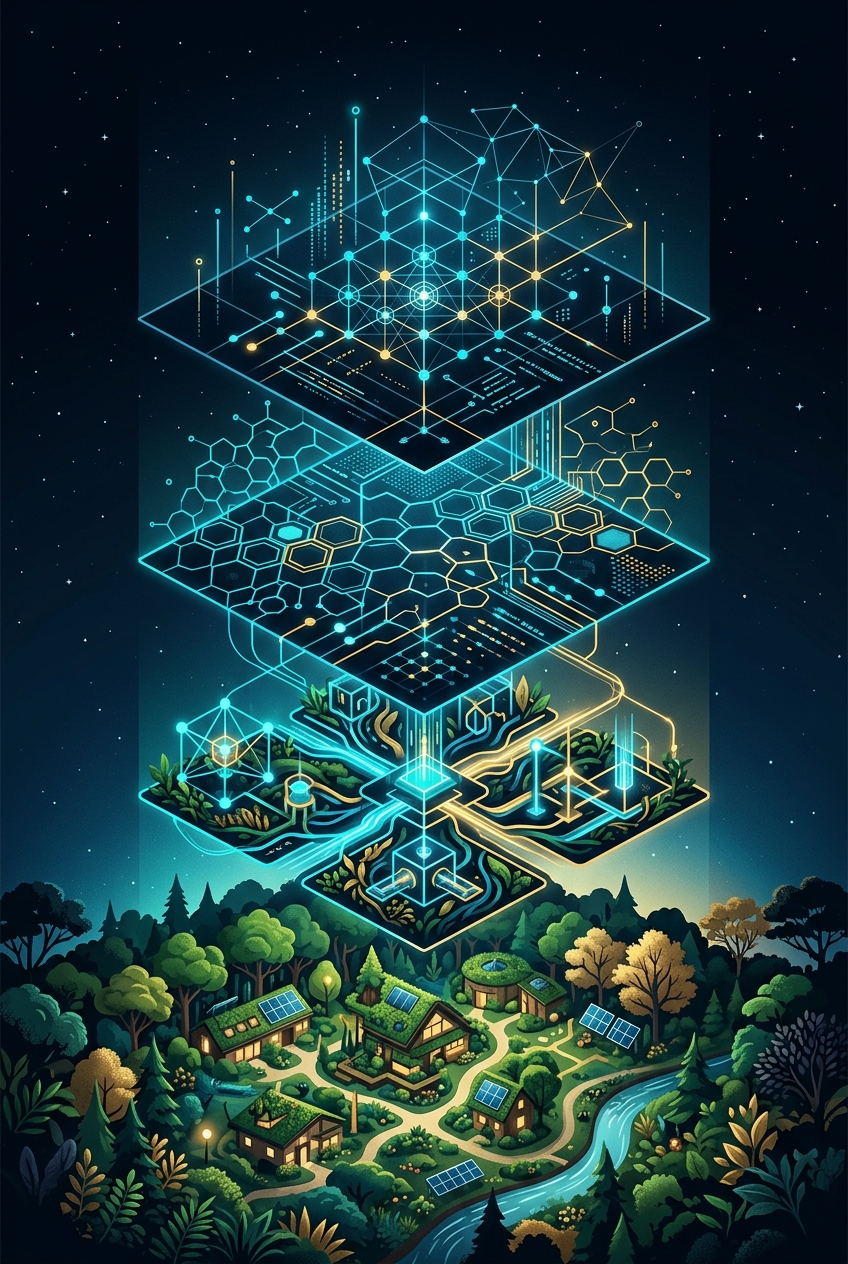
\includegraphics[width=\paperwidth,height=\paperheight,keepaspectratio=false]{cover_v2.jpg}
        };
        \node[anchor=north, yshift=-3cm] at (current page.north) {
            \scalebox{2.1}{\Huge \textbf{\textcolor{white}{\fontfamily{qag}\selectfont The Sovereign Stack}}}
        };
        \node[anchor=south, yshift=2.5cm] at (current page.south) {
            \scalebox{2}{\Large \textbf{\textcolor{white}{\fontfamily{qag}\selectfont The Collective}}}
        };
    \end{tikzpicture}
    
    \clearpage
    % Page 2: Blank inner cover
    \thispagestyle{empty}
    \null
    \clearpage
    
    % Page 3: Inner Title Page
    \thispagestyle{empty}
    \begin{center}
        \vspace*{4cm}
        {\scalebox{1.6}{\textbf{The Sovereign Stack}}} \\[1cm]
        {\Large \textit{A Blueprint for Cybernetic Ecology and Mutual Aid}} \\[3cm]
        {\Large \textbf{The Collective}} \\[3cm]
        \vfill
        {\large Version 1.0 (Initial Draft)} \\[0.2cm]
        {\large Cascadia Bioregion, 2026}
        \vspace*{3cm}
    \end{center}
    \clearpage
\end{titlepage}
\tableofcontents

\chapter{Preface: The Physics of Exhaustion}

\epigraph{``It is not the state that gives us life, nor the market that sustains it, but the unbroken chain of kinetic solidarity---the soil, the sun, and the hands of our neighbors.''}{--- \textit{Internal Node Charter, 2026}}

We are profoundly exhausted. 

This exhaustion is not merely psychological; it is explicitly thermodynamic. The legacy architecture of the twenty-first century---what we now call the Legacy Stack---was engineered from the ground up as an extractive engine. It atomizes the human animal into a nuclear, hyper-financialized unit, deliberately severing our intrinsic ties to the physical watershed, to the rhythms of the seasons, and to each other. It forces us to outsource our survival to brittle, globalized supply chains and centralized, opaque state monopolies that optimize for profit extraction rather than human resilience. 

As Byung-Chul Han observes, late-stage capitalism transitions from a disciplinary society to an achievement society, where we internalize the demand for endless growth until we literally collapse from within \parencite{han2015}. We become our own taskmasters, burning our cognitive and physical exergy to fuel systems that offer no genuine nourishment in return. When the centralized power grid fails, we freeze in our smart homes. When the just-in-time supply chain fractures, we starve amidst abundance. When we experience the inevitable emotional burnout of this unnatural arrangement, we are pathologized, institutionalized, or further commodified by a wellness industry that treats the symptoms while ignoring the structural disease. 

Mark Fisher described this suffocating lack of horizon as \textit{Capitalist Realism}---the pervasive, paralyzing sense that it is easier to imagine the end of the world than the end of capitalism \parencite{fisher2009}. But we must understand that this inability to imagine an alternative is not a failure of human spirit; it is merely a failure of infrastructure. We cannot think our way out of a trap built of steel and silicon; we must build a new material reality.

\textit{The Sovereign Stack} is a technical manual for constructing that reality. In the following chapters, you will read about Directed Acyclic Graphs (DAGs), Ed25519 cryptography, Conflict-Free Replicated Data Types (CRDTs), and voxel-based thermodynamic engines. But before we touch a single line of C++ or instantiate a single Digital Twin, we must fiercely anchor these technicalities in their true human purpose. 

Technology in The Collective is not designed to abstract us away from reality, as the legacy internet did with its endless feeds and disembodied avatars. It is designed to embed us irrevocably deeper into the dirt, the water, and the community. 

We draw heavily upon the anarchist tradition of Peter Kropotkin, who demonstrated mathematically and historically that mutual aid, not ruthless competition, is the primary factor of evolutionary survival \parencite{kropotkin1902}. We operationalize the polycentric governance models of Elinor Ostrom, proving that local communities can manage complex commons---from aquifers to fabrication labs---without the tragedy of depletion or the violent intervention of the state \parencite{ostrom1990}. And we structure our collective data utilizing the management cybernetics of Stafford Beer, treating the community as a Viable System Model (VSM)---a decentralized, biological nervous system capable of autonomous homeostasis \parencite{beer1972}.

This book translates those towering theoretical frameworks into a workable, localized reality. It is a guide to building a Node: a digitally orchestrated, physically sovereign neighborhood capable of housing, feeding, and healing its citizens, totally decoupled from the legacy matrix. It is time to stop surviving the machine, and start building the garden.


\mainmatter

\chapter{The Anatomy of a Node}

\epigraph{``In a truly rational society, the concept of a 'network' is not a digital phenomenon, but an ecological one. The separation of the social from the environmental is a lethal illusion.''}{--- \textit{Murray Bookchin} \parencite{bookchin1982}}

To understand The Collective, you must stop thinking of technology as screens and start thinking of it as infrastructure. The Node is the base unit of our architecture. It is not a website or a social network; it is a physical bioregion---a watershed, a city block, an old suburban cul-de-sac---overlaid with a localized digital nervous system.

If you have ever tried to organize a community garden, share tools with neighbors, or coordinate childcare, you know the friction involved. Text chains become chaotic. Obligations become asymmetrical. Resentment builds. The community fractures.

The Sovereign Stack utilizes the mathematics of distributed computing to eliminate this interpersonal friction. It translates the abstract concepts of fairness, resource allocation, and trust into automated, un-gameable protocols. 

Before we deploy a single sensor or compile a single WebAssembly module, we must fully grasp the anatomy of the organism we are building. This chapter serves as your foundational blueprint for the Node. 

First, we will examine \textbf{The Historical Rupture}, diagnosing exactly why the legacy internet, built on assumptions of infinite extraction, inevitably collapsed into surveillance capitalism and systemic burnout. 

Once the failure modes are mapped, we will dissect \textbf{The Seven Layers of Sovereignty}, a rigorous, OSI-inspired architectural stack designed to ensure our digital tools remain strictly bound by the thermodynamic realities of the earth. 

Following the architecture, we will reveal \textbf{The Oasis Strategy}---the Trojan Horse approach of using a local-first video game to gently onboard overwhelmed populations into the complexities of cybernetics. 

We will then explore \textbf{Scenario Driven Development (ScDD)}, the rigorous engineering methodology we use to forge the Oasis Engine against the simulated, statistical pressures of the extractive old world. 

Finally, in \textbf{Translating Cybernetics to Human Flourishing}, we will establish our ultimate mission: how this entire technical apparatus serves only to absorb the cognitive load of survival, giving the human system the structural permission to finally rest.

\section{The Historical Rupture}

Before deploying a Node, we must understand exactly why prior technological interventions failed to save us, and how the original promise of the internet was inverted. 

The early architecture of the web was conceived as a decentralized, academic commons. Protocols like TCP/IP and HTTP were designed to route around damage, assuming a peer-to-peer topology where every node had equal standing. However, because these protocols lacked native layers for identity, trust, and value transfer, a vacuum was created. This vacuum was rapidly filled by centralized corporate platforms. We witnessed the greatest enclosure of a commons in human history. 

As Shoshana Zuboff details, this new architecture was hijacked to extract \textit{behavioral surplus} \parencite{zuboff2019}. Human experience itself was strip-mined, quantified, and sold to third-party markets. Surveillance Capitalism does not merely track us to serve advertisements; it fundamentally re-engineers our behavior, atomizing communities by replacing organic, local trust with algorithmic dependency on distant server farms. We stopped talking to our neighbors and started querying the Cloud.

This behavioral extraction is inextricably linked to a profound thermodynamic delusion. The legacy internet relies on a user interface of frictionless magic, deliberately hiding the massive physical violence required to sustain it. Behind the glass screens of our devices lies a brutal supply chain of rare earth mining, exploited labor, and hyperscale data centers that consume gigawatts of power. The prevailing logic of the legacy system assumed infinite planetary exergy, structurally decoupling the digital economy from the biological carrying capacity of the earth.

It optimized for supply and demand pricing, deliberately ignoring negative externalities, allowing extractive algorithms to deplete ecosystems until they collapsed. By failing to integrate the physical limits of the Earth system into their fundamental architectures, these technologies became accelerators of entropy rather than tools for homeostasis. As system theorist Donella Meadows noted, attempting to manage a complex system by maximizing a single variable---like profit, engagement, or infinite growth---inevitably leads to the destruction of the system itself \parencite{meadows2008}. 

This structural sociopathy poses a terrifying risk as our legacy systems become increasingly automated. In Daniel Suarez's prescient techno-thriller \textit{Daemon}, we are given a stark illustration of an algorithmic society operating with ruthless efficiency but entirely devoid of a human-centric ethical framework \parencite{suarez2006}. When complex systems optimize strictly for their own programmatic survival, citizens are reduced to mere mechanical appendages---biological subroutines serving a dead machine. 

Faced with this existential threat, the historical impulse is often violent convolution---the ``Revolutionary Method.'' Yet, attempts to dismantle the legacy machine through direct political or physical confrontation inevitably fall apart. Anti-capitalist activists have historically struggled against a system that is not merely an ideological opponent, but a deeply entrenched, structural public health crisis. As Peter Joseph argues in \textit{The New Human Rights Movement}, the socioeconomic architecture of capitalism is inherently violent and cannot be solved through policy reforms or physical uprisings that leave the underlying incentive structure intact \parencite{joseph2017new}. You cannot dismantle a globally distributed, algorithmic hyperobject using the organizational tools of the nineteenth century. As Hannah Arendt observed, the sudden violent collapse of authority rarely results in liberation; instead, the resulting revolutionary vacuums are swiftly filled by new tyrants, and the underlying apparatus of extraction simply changes management \parencite{arendt1963}. The legacy system is too deeply entrenched in our logistics, our food supply, and our psychology to be destroyed head-on without causing catastrophic collateral damage to the vulnerable.

Instead of a frontal assault, The Collective adopts a structuralist approach to obsolescence. The anarchist philosopher Gustav Landauer famously noted that the state is not a physical structure that can be smashed, but rather a set of relationships between human beings; we destroy it by contracting other relationships and behaving differently \parencite{landauer2010}. Translating this to the digital era, Buckminster Fuller's engineering axiom holds true: to change something, you build a new model that makes the existing model obsolete \parencite{fuller1981}. 

This structuralist ethos is strongly echoed in Peter Joseph's recent framework, \textit{Integral} \parencite{joseph_integral}. Like The Collective, \textit{Integral} takes its own rigorous approach to architecting a transition away from the market economy. Within this space of systems design, there is no rivalry or competition. It is highly probable that the economic models expressed in \textit{Integral} can be directly translated into the Sovereign Stack, utilizing our digital architecture to implement their systemic goals. The legacy system cannot be overthrown; it must be starved of our kinetic energy and rendered obsolete through the collaborative construction of parallel, superior infrastructure. 

This brings us to our Trojan Horse. We cannot ask a burned-out, exhausted populace to suddenly adopt a complex, rigorous cybernetic lifestyle out of pure moral duty. Instead, we bootstrap the sovereign reality by embedding it within the shell of the old world. By utilizing a legal proxy to interface safely with the legacy state, and deploying our physics engine (Oasis) as a gamified shadow-simulator to safely model local ecology, we slip the seeds of a new world past the defenses of the old. 

The historical rupture, therefore, is this: we built a planetary nervous system that is structurally sociopathic. It feels no pain when a forest burns or a community fractures. The Sovereign Stack, detailed in the following Seven Layers, is our blueprint for building a nervous system that can finally feel the fire, pull its hand away, and heal the burn.

\section{The Seven Layers of Sovereignty}

To make the transition from the legacy world to the sovereign world comprehensible, and to ensure that catastrophic failures in one domain do not cascade through the entire system, we divide our operational architecture into a strict seven-layer stack. 

This architecture draws direct inspiration from the Open Systems Interconnection (OSI) model, formulated in 1980 to standardize and abstract telecommunication and computing systems \parencite{zimmermann1980}. While the original OSI model was designed to safely route digital data packets, The Sovereign Stack is designed to safely route thermodynamic exergy, legal liability, and human labor. 

Before defining the stack itself, we must establish the two inviolable rules governing this architecture:
\begin{enumerate}
    \item \textbf{Strict Adjacency:} A layer can only interact with the layers directly above or below it. There is no bypassing. A semantic human command (Layer 6) cannot directly actuate a physical water valve (Layer 1); the intent must compile downward step-by-step through governance policy, local orchestration, ledger validation, and edge telemetry. This strict traversal prevents the disastrous security vulnerabilities and physical hazards inherent in legacy systems.
    \item \textbf{Total Encapsulation (Domain Isolation):} A layer is strictly concerned with its own internal domain and carries absolutely no contextual understanding of the layers it interfaces with. The Thermodynamic Ledger (Layer 3) does not know what a ``garden'' or a ``citizen'' is; it only understands cryptographic proofs and exergy metrics. Conversely, the Governance layer (Layer 5) does not understand the voltage of a solar panel. 
\end{enumerate}

By rigidly enforcing this encapsulation, we guarantee that the mechanistic logic of the lower layers never corrupts the semantic meaning of human life in the higher layers. The lower layers are bound by the merciless physics of dirt and heat; the higher layers interface with complex human intent and legacy state bureaucracy.

\begin{description}
    \item[Layer 1: Physical Reality] \hfill \\
    \textbf{Domain:} Mass, Energy, and Kinetic Labor. \\
    \textbf{Responsibilities:} The ultimate ground truth of the system. Responsible for housing the biological carrying capacity, the physical hardware (3D printers, biochar kilns), and human physical labor. It enforces the inescapable boundaries of thermodynamics. Nothing in the digital realm matters if it cannot survive a power outage or a winter storm.

    \item[Layer 2: The Digital Twin (Telemetry)] \hfill \\
    \textbf{Domain:} Sensors, Actuators, and Signal Processing. \\
    \textbf{Responsibilities:} The sensory nervous system. Responsible for ingesting raw physical data (temperature, weight, moisture) via localized, air-gapped IoT meshes (LoRaWAN) and converting it into cryptographic signals. It is strictly responsible for observation and actuation, possessing no decision-making logic of its own.

    \item[Layer 3: The Thermodynamic Ledger] \hfill \\
    \textbf{Domain:} Consensus, Value Tokenization, and Exergy Accounting. \\
    \textbf{Responsibilities:} The fundamental accounting system. Responsible for maintaining a decentralized, conflict-free record of physical exergy (Joules, Watts, Biomass). It abandons fiat currency, utilizing an Ecological Replacement Cost (ERC) asymptote to automatically reject any transaction that would mathematically lead to ecological collapse.

    \item[Layer 4: The Orchestrator] \hfill \\
    \textbf{Domain:} Automation, State Machines, and Workflow Execution. \\
    \textbf{Responsibilities:} The algorithmic heart. Responsible for deterministically matching human needs with physical resources through executable Business Process Model and Notation (BPMN) workflows. It acts as an embedded WebAssembly (WASM) executor that compiles abstract governance policies into localized, physical action.

    \item[Layer 5: Governance \& The Web of Trust] \hfill \\
    \textbf{Domain:} Reputation, Access Control, and Polycentric Policy. \\
    \textbf{Responsibilities:} The community immune system. Responsible for calculating cryptographic trust through graph theory. It determines who has the right to access sensitive tools, vulnerable community members, or hazardous materials, thereby digitally enforcing Ostrom's principles for managing the commons without police or credit scores.

    \item[Layer 6: Semantic Intent] \hfill \\
    \textbf{Domain:} Human-Computer Interface, Knowledge Graphs, and Language. \\
    \textbf{Responsibilities:} The translation layer between human desire and machine execution. Responsible for structuring complex, ambiguous human needs (``I need to mediate a dispute'' or ``I am hungry'') into verifiable, machine-readable ontologies (JSON-LD, PROV-O) that can be safely passed downward to the policy and orchestration engines.

    \item[Layer 7: The Legacy Proxy] \hfill \\
    \textbf{Domain:} Fiat Currency, Legal Entities, and State Interfacing. \\
    \textbf{Responsibilities:} The ablative shield. Responsible for translating the internal sovereign operations into a format the legacy world understands. It files permits, pays fiat taxes, and holds corporate charters (like a Social Purpose Corporation), absorbing the friction of state bureaucracy so the internal Node remains autonomous and perfectly insulated.
\end{description}

\subsection{Layer 1: Physical Reality}

The foundational layer of The Sovereign Stack is not written in code, but in the immutable laws of thermodynamics, gravity, and biology. In legacy technological systems, digital platforms operated under the delusion of infinite growth and infinite energy, structurally decoupling the economy from the biological carrying capacity of the Earth. Layer 1 exists to shatter this delusion. It serves as the ultimate ground truth, anchoring the entire digital architecture to the physical realities of dirt, heat, and human kinetic labor. It ensures that the digital nervous system can never mathematically demand more exergy than the local biome can sustainably provide.

Because this layer sits at the absolute bottom of the stack, it possesses no downward interface. It is the basilar reality of Nature itself. For The Collective, this foundational layer can only be approached in two ways: it must be \textit{Understood} and it must be \textit{Simulated}. Understanding is the domain of Science---the rigorous modeling of the thermodynamic and biological rules governing the local watershed or soil microbiome. Simulation is the domain of the Oasis Engine. Before we execute a workflow that alters this physical layer, Oasis models the outcome---initially operating as a gamified interface, but ultimately serving as a critical shadow-simulator to test ecological interventions safely before they are physically deployed.

Upward, Layer 1 interfaces with Layer 2 (The Digital Twin) strictly through observable physical phenomena. The ambient heat of a compost pile, the mass of harvested potatoes, or the moisture content of topsoil are the only signals this layer provides to the stack. Conversely, the stack's signals back into Layer 1 are the physical interventions carried out by actuators---a water valve opening, a solar relay tripping, or the physical sweat and labor of a human being acting upon the earth.

Consider the operation of a community biochar kiln processing agricultural waste. In a legacy system, the kiln's operation might be modeled purely in financial terms, ignoring the realities of heat loss, carbon sequestration, and human fatigue. In The Sovereign Stack, Layer 1 dictates the absolute boundaries of this workflow. The physical tolerances of the steel kiln, the exact weight and moisture of the biomass, and the biological calories burned by the human citizen operating it define the absolute maximum carrying capacity for that event. There is no negotiating with Layer 1; it is the physical bedrock upon which all subsequent abstractions must justify their existence.

\subsection{Layer 2: The Digital Twin (Telemetry)}

If Layer 1 is the physical body of the biome, Layer 2 serves as its sensory nervous system. In the legacy internet of things (IoT), the act of measuring physical reality was inherently an act of surveillance; sensors were designed to ping centralized corporate cloud servers, extracting data from the local environment to feed distant behavioral models. Layer 2 is engineered to replace this panopticon with self-determined, strictly localized observation. It exists to safely and securely translate raw physical reality into digital signals without ever leaking that data outside the sovereign boundaries of the Node.

Because its sole purpose is observation and actuation, Layer 2 contains absolutely no decision-making logic or policy engines. Downward, it reaches into the physical reality of Layer 1 through hardware sensors and effectors---thermocouples embedded in compost, weight scales under grain silos, and servos attached to water lines. Upward, strictly enforcing the law of adjacency, it interfaces exclusively with the Thermodynamic Ledger (Layer 3) by broadcasting cryptographically signed MQTT or CoAP payloads over air-gapped, peer-to-peer LoRaWAN or WiFi meshes. 

Consider the interaction of a simple soil moisture sensor. The hardware detects a 20\% saturation level in the local permaculture guild---a physical state belonging to Layer 1. The sensor's only job is to format this reality into a lightweight JSON payload, sign it with its unique cryptographic key, and broadcast it upward to Layer 3. It does not decide if the soil is too dry, nor does it authorize the release of water. It simply reports the thermodynamic truth of the dirt to the ledger, waiting for an actuation command to eventually cascade back down the stack once the higher layers have evaluated the policy and cryptographically allocated the necessary exergy.

\subsection{Layer 3: The Thermodynamic Ledger}

At the core of the legacy world's systemic collapse was a fatal abstraction: fiat currency. By completely decoupling the representation of value from the physical constraints of reality, legacy economies were incentivized to strip-mine the earth and exploit human labor without ever registering the true thermodynamic cost on their balance sheets. Layer 3, the Thermodynamic Ledger, exists to permanently close this loophole. It serves as the fundamental accounting system of the Node, completely abandoning fiat currency in favor of a decentralized, tamper-proof ledger of physical exergy. By embedding an Ecological Replacement Cost (ERC) asymptote directly into its protocol, this layer automatically rejects any transaction that would mathematically lead to ecological collapse, ensuring the local economy operates strictly within the boundaries of physics.

Following the law of adjacency, Layer 3 acts as the vital bridge between the physical realities reported by the sensors below it and the automated logic sitting above it. Downward, it ingests cryptographically signed telemetry payloads from Layer 2, serving as the sole verifier of physical truth. Upward, it interfaces with the Orchestrator (Layer 4) by exposing the current balance of available Value Tokens. It maintains this state across the decentralized mesh without relying on the energy-intensive Proof-of-Work blockchains of the old internet, utilizing instead highly efficient Conflict-Free Replicated Data Types (CRDTs) to guarantee eventual consistency.

To illustrate this mechanism, imagine a community solar array that has just generated 500 Joules of surplus exergy. The physical generation is recorded by Layer 2 and passed upward as a secure telemetry payload. The Thermodynamic Ledger receives this data, verifies the cryptographic signature of the sensor, and validates that the energy was actually generated. It then permanently mints the corresponding Value Tokens to the community wallet, propagating the updated ledger state across the local libp2p Gossipsub network. This instantly synchronizes the newly generated energetic wealth across all nodes in the mesh while cryptographically preventing double-spending. Consequently, Layer 4 is provided with a perfectly accurate, physics-bound budget ready to be allocated to future workflows.

\subsection{Layer 4: The Orchestrator}

If Layer 2 is the sensory nervous system and Layer 3 is the metabolic budget, Layer 4 acts as the operational brain of the Node. In legacy systems, coordinating complex logistics---matching human needs with physical resources---required constant, exhausting managerial oversight, inevitably leading to the very burnout The Sovereign Stack seeks to cure. The Orchestrator exists to automate this cognitive load. It is an algorithmic engine designed to execute deterministic workflows, ensuring that community coordination happens seamlessly, reliably, and without requiring human micro-management.

Adhering strictly to the law of adjacency, the Orchestrator sits directly between the financial truths of the Ledger (Layer 3) and the polycentric policies of Governance (Layer 5). Upward, it receives approved, executable policies from Layer 5, which dictate what the community has collectively decided to do. Downward, it queries Layer 3 to verify if there is sufficient thermodynamic budget (Value Tokens) to actually execute those decisions. If the budget exists, the Orchestrator initiates the workflow, issuing token transfers and cryptographically signing actuation requests that are handed downward for processing. 

To achieve this, Layer 4 operates as an embedded WebAssembly (WASM) executor running complex Business Process Model and Notation (BPMN) state machines. Consider a community decision to irrigate a permaculture field during a drought. The Orchestrator receives the validated policy from Layer 5. It queries Layer 3 and confirms there is a surplus of solar exergy tokens available to run the water pumps. The WASM engine then deterministically executes the BPMN workflow: it transfers the required tokens to the water guild's address on the Ledger, and passes an actuation command down to Layer 3, which in turn cascades the command to the Layer 2 servos to open the valves for exactly ten minutes. The human citizens are entirely relieved of the burden of manual coordination; they simply watch the water flow.

\subsection{Layer 5: Governance \& The Web of Trust}

Every society requires an immune system to protect its commons from malicious actors, incompetence, or tragic depletion. In the legacy world, this function was violently outsourced to coercive state police forces and opaque, centralized corporate credit scores. Layer 5, Governance and The Web of Trust, replaces these mechanisms with a localized, cryptographic immune system. By digitizing Elinor Ostrom's polycentric principles for managing the commons, this layer calculates reputation and access organically, ensuring that shared resources are managed collaboratively without centralized control or the threat of state violence.

Following the architecture's strict encapsulation, Layer 5 is entirely blind to fiat money or raw thermodynamic telemetry; its sole domain is cryptographic reputation and policy validation. Upward, it receives structured semantic requests from Layer 6 (Semantic Intent) and evaluates them against the community's decentralized graph data. Downward, once a policy or request is validated against the Web of Trust, Layer 5 provides a cryptographic attestation of approval to the Orchestrator (Layer 4), authorizing the state machine to safely execute the workflow.

Consider a scenario where a citizen requests access to a hazardous piece of community infrastructure, such as an industrial CNC machine. Instead of relying on a centralized bureaucratic license, Layer 5 traverses the local Web of Trust graph. It verifies whether three trusted members of the fabrication guild have cryptographically attested to the citizen's safety and competence. If the graph-theoretic threshold is met, the layer automatically issues a multi-signature approval and passes it downward to Layer 4. The citizen is granted access, not through coercion or hierarchy, but through verifiable, peer-to-peer solidarity.

\subsection{Layer 6: Semantic Intent}

If the lower layers of the stack are governed by the rigid mathematics of thermodynamics and state machines, Layer 6 is where the architecture finally interfaces with the messy, ambiguous reality of human desire. In legacy tech ecosystems, users are often forced to adapt their behavior to the inflexible schemas of corporate databases, clicking through prescriptive menus that flatten human experience. The Semantic Intent layer completely reverses this dynamic. It exists to allow non-technical citizens to interact with a highly complex cybernetic system using natural language and intuitive interfaces, acting as the ultimate translator between human needs and machine execution. 

Adhering to the stack's strict encapsulation, Layer 6 does not know how many joules of energy reside in a battery, nor does it know the cryptographic hash of a governance policy. Its sole domain is language and knowledge graphs. Downward, it interfaces with Governance (Layer 5) by structuring abstract human intents into standardized, machine-readable formats. Upward, it translates aggregated community needs to the Legacy Proxy (Layer 7) whenever an intent requires interfacing with the external capitalist world.

Consider a citizen who opens a local Node application and simply types, ``I am exhausted and need someone to watch my children on Tuesday.'' The Semantic Intent layer utilizes standard W3C ontologies, such as JSON-LD and PROV-O, to parse this unstructured human cry for help into a verifiable knowledge artifact. It formats the intent into a specific semantic structure---identifying the temporal constraint, the required trust parameters for childcare, and the energetic token budget available. It then passes this structured artifact downward to Layer 5 for governance evaluation. The citizen never sees a line of code or a cryptographic key; they only experience a system that listens, understands, and organically mobilizes the community to provide care.

\subsection{Layer 7: The Legacy Proxy}

No matter how sovereign a Node becomes, it still exists within a geographic territory claimed by the legacy state, and it still requires materials manufactured by legacy global supply chains. If the internal cybernetic layers were directly exposed to the external world, the Node would be quickly crushed by bureaucratic friction, fiat taxation, or corporate surveillance. Layer 7 exists solely to act as an ablative shield. It is the tactical outer hull that absorbs the legal threats, paperwork, and financial volatility of the old world, ensuring that the internal sovereign mesh remains perfectly insulated and autonomous. 

By design, Layer 7 is the only layer permitted to touch fiat currency or state bureaucracy. Downward, it interfaces with Semantic Intent (Layer 6), receiving aggregated community needs that simply cannot be fulfilled by local thermodynamic resources. Outward, it interfaces with the legacy matrix---filing state tax returns, managing fiat banking APIs, and holding the legal deeds to the Node's physical land. It typically takes the form of a legally recognized entity, such as a Social Purpose Corporation or a community land trust. It essentially wears a ``capitalist mask'' to trick the legacy system into leaving the Node alone.

Crucially, this mask is not merely defensive; it is actively parasitic to the old world. Layer 7 offers The Collective the tactical ability to ``leech'' resources from the legacy system. By taking surplus internal capacities or specialized labor and dressing those Layer 6 intents up as standard commercial services---such as software consulting, data hosting, or agricultural exports---Layer 7 can seamlessly sell them on the open market. It extracts fiat currency from legacy corporations, metabolizes that fiat through the proxy, and uses it to purchase the physical hardware required to accelerate the Node's total untethering from the system.

Consider a scenario where the community must purchase physical solar panels from an external corporate supplier to expand its energy capacity. The external corporation expects to be paid in fiat currency and requires a legal tax ID. Layer 7 executes the purchase using its fiat reserves and files all necessary import documents. The external supplier is completely unaware that they are selling to a decentralized thermodynamic collective; they never see the local Web of Trust (Layer 5), and they never gain access to the internal Thermodynamic Ledger (Layer 3). Layer 7 successfully translates the transaction, protecting the internal cybernetic garden from the extractive logic of the world outside.


\section{The Oasis Strategy: From Simulation to Reality}

None of the formidable technical architecture of The Sovereign Stack matters if we cannot successfully deploy it into the hands of exhausted, overwhelmed people. We cannot expect a population already suffering from severe capitalist burnout to eagerly read documentation on thermodynamics, BPMN automation, or Conflict-Free Replicated Data Types (CRDTs). If we demand ideological purity and technical mastery upfront, we will fail. 

Therefore, The Collective is not introduced as a political revolution or a daunting engineering project. It is introduced as a video game. 

This is the Oasis Strategy. The Trojan Horse of our architecture is the Oasis Engine: a high-performance, local-first voxel simulator built in C++20 and compiled to WebAssembly (WASM) to run effortlessly in a standard web browser. At first glance, it is simply a game about building resilient, ecologically balanced settlements. But beneath the surface, Oasis is fundamentally running the exact cybernetic logic of The Sovereign Stack.

When a player builds an automated irrigation system in the game, the engine generates real Layer 4 BPMN XML to execute the logic. When players collaborate in multiplayer, they are not connecting to a centralized corporate server; their local clients are syncing state via the exact libp2p Gossipsub and CRDT mechanics that power the Layer 3 Thermodynamic Ledger. By simply playing the game, citizens naturally internalize the laws of exergy, the boundaries of carrying capacity, and the mechanics of polycentric governance without ever reading a manual.

The true genius of the Oasis Engine, however, reveals itself when the game transcends the screen. Once a community is ready to physically construct a Genesis Node in the real world, Oasis does not become obsolete. Instead, it seamlessly pivots from a virtual game into a ``Shadow Simulator.'' 

By connecting to the physical hardware of Layer 1 and the telemetry of Layer 2, the exact same engine that the citizens used to play the game now consumes live data from their real-world sensors. It models physical workflows---such as the fluid dynamics of a real rainwater catchment system---safely in the digital twin \textit{before} any actuation commands are sent down the stack. 

We use the familiar, safe paradigm of a video game to gently guide a population out of digital escapism and into physical empowerment, utilizing the Oasis Engine as the crucial bridge between the virtual and the thermodynamic.
\section{Scenario Driven Development}

To construct an architecture as complex and consequential as The Sovereign Stack, traditional software engineering methodologies are insufficient. When code directly orchestrates physical water pumps (Layer 2) or calculates thermodynamic survival budgets (Layer 3), a simple software bug is no longer a localized inconvenience; it is a physical, ecological failure. To safely engineer the Oasis Engine and the broader stack, The Collective employs a methodology we call \textit{Scenario Driven Development (ScDD)}.

ScDD is an evolutionary successor to the software engineering paradigms of the early 21st century. In 2002, Kent Beck formalized Test-Driven Development \parencite{beck2002test}, forcing engineers to write failing tests before writing production code to ensure isolated, mechanical correctness. A few years later, Dan North introduced Behavior-Driven Development \parencite{north2006introducing}, shifting the focus from mechanical tests to human-readable behavioral specifications, ensuring the software actually met the semantic desires of its users. 

Scenario Driven Development takes this progression to its ultimate, physical conclusion. While TDD tests abstract code logic, and BDD tests human behavior, ScDD tests \textit{thermodynamic and ecological outcomes}. 

Before a single line of C++20 or WASM is written for the Oasis Engine, engineers do not write a unit test; they construct a rigorous, physical \textit{Scenario}. A Scenario is a mathematically defined ecological problem bounded by the laws of physics. For example: \textit{``A permaculture guild spanning two acres is experiencing a 15\% reduction in historical rainfall; the system must maintain a minimum soil moisture of 20\% without exceeding its local exergy budget of 10,000 Value Tokens per week.''}

Once the Scenario is defined, it is loaded into the Oasis Engine's shadow-simulator. Crucially, a Scenario does not exist in a vacuum; it must also rigorously map the existing legacy impact on that specific biome. The engine simulates the extractive forces of the surrounding capitalist world---such as municipal water drainage, industrial pollution runoff, or fiat inflation---representing them as a continuous statistical pressure bearing down on the Node's boundaries. 

The software is then developed iteratively against this hostile scenario. The code is only considered ``passing'' when the simulated Thermodynamic Ledger (Layer 3) balances, and the simulated telemetry (Layer 2) confirms the ecological requirement is met despite the legacy pressure, all without violating the Ecological Replacement Cost (ERC) asymptote. 

This strategy inherently forces the software to conform to the biological carrying capacity of the real world while actively surviving the entropy of the old world. It prevents the development of ``features'' that are digitally impressive but ecologically fragile. By utilizing Scenario Driven Development, the Oasis Engine is continuously forged in the crucible of simulated physical reality, ensuring that when the video game finally transitions into a real-world Orchestrator, the community can trust it with their lives.


\section{Translating Cybernetics to Human Flourishing}

None of this technical architecture matters if it does not serve a profoundly human purpose. The Sovereign Stack is not built to create a rigid technocratic utopia; it is built to cure the burnout, isolation, and ecological dread that define modern life. 

By automating the logistics of survival via the Orchestrator (Layer 4) and bounding those logistics within the thermodynamic limits of the earth via the Ledger (Layer 3), the Node frees the human mind from the constant, exhausting calculus of capitalist extraction. In legacy systems, citizens are forced to act as hyper-vigilant micro-managers of their own survival. In The Collective, the architecture shoulders this burden. The digital twin watches the crops; the orchestrator routes the water; the Web of Trust mediates the risk; the legacy proxy absorbs the state's violence. 

Ultimately, this is our mission statement: The cybernetic system must absorb the friction of reality, so that the human system can finally begin to flourish. By delegating the mechanics of survival to a localized, physics-bound intelligence, human beings are allowed to return to what we are biologically and sociologically designed to do. We are freed to build culture, to create art, to care for our elders, and to reconnect deeply with the land. The technology is merely the soil; human flourishing is the harvest.


\chapter{Layer 1: The Physics of Reality}

In the legacy architecture of the internet, physical reality was treated as an infinite, abstract substrate---a silent void from which rare earth metals and electricity could be endlessly extracted to power data centers. In The Sovereign Stack, Layer 1 fundamentally reverses this relationship. Layer 1 is not a software protocol; it is the absolute biological and thermodynamic ground truth of the Node. It is the soil microbiome, the tensile strength of steel, the heat of a biochar kiln, and the biological calories burned by human labor. 

Because Layer 1 is physical reality itself, the digital stack cannot issue direct commands to it in the way a CPU commands a hard drive. Instead, the architecture must interface with the physical world through a precise sequence of translation.

In this chapter, we explore how The Collective navigates this boundary. We begin with \textbf{Understanding}---the necessity of rigorously codifying the raw thermodynamic truths of the Earth into compressed, executable formats. We then explore how this knowledge feeds the \textbf{Simulation} layer, utilizing the Oasis Engine as a digital twin to safely stress-test our ecological and architectural assumptions against legacy pressures. Finally, we examine \textbf{The Genesis Transition}, the critical pivot where the simulation ceases to be a hypothetical game and irreversibly actuates into physical, biological reality.

\section{Understanding: Codifying the Architecture of Truth}

To interact meaningfully with Layer 1, a Node must first be capable of understanding it. However, this Understanding is not a semantic human intent from Layer 6, nor is it simply a list of automated tasks. It is rigorously codified scientific knowledge---the mathematical abstractions, biological models, and thermodynamic rules that map specifically and exclusively to the physical reality of Layer 1. 

The primary challenge lies in the representation and efficient storage of this vast, complex knowledge. If the system is to accurately emulate the fluid dynamics of a local watershed or the nutrient cycling of a permaculture guild, these models must be stored in formats that are highly compressed and readily executable. 

The storage and distribution of this codified knowledge is the explicit responsibility of the lower stack (Layers 1 through 4). The raw physical truth is sensed at Layer 2, but the scientific models that contextualize that truth are distributed across the mesh using the CRDT state-syncs of the Thermodynamic Ledger (Layer 3) and embedded directly into the deterministic WebAssembly (WASM) execution environment of the Orchestrator (Layer 4). The knowledge of physics is not trapped in a static database; it is codified directly into the localized network that orchestrates the Node. 

However, scientific understanding is never static. Biomes shift, ecosystems adapt, and our mathematical abstractions must continually evolve. Therefore, the maintenance and governance of this knowledge is handled by the upper stack (Layers 4 through 7). When a community observes that their soil capacitance behaves differently than the current model dictates, they must update the codified knowledge without breaking the physical infrastructure. 

This is where the Oasis Engine serves a critical function. Operating as a highly advanced simulation environment at the top of the stack, Oasis provides the visual and mechanical testing ground for new scientific models. A citizen can propose an updated mathematical abstraction, test it within the Oasis simulator, and submit it for polycentric governance. Layers 5 and 6 mediate the trust and semantic meaning of the proposal. Once consensus is reached, the new understanding of physical reality cascades back down, updating the modules in Layer 4 and synchronizing across the Layer 3 ledger. In this way, the Node maintains a living, constantly evolving codification of the natural world.

\subsection{Abstracting the Right Things: The Exergy Model}

The ambition to codify the physical world is inherently daunting. The Collective seeks to mathematically map an immense vastness of human knowledge, encompassing physical, chemical, biological, psychological, and even localized social phenomena. The goal is to quantify these interactions with enough rigor to fully automate the logistics of human survival, thereby freeing our communities to live entirely outside the extractive economic-political landscape. The Collective operates on a foundational premise: if we can abstract the \textit{right} things, we can render the legacy system obsolete. 

Crucially, abstracting the right things means knowing what to violently exclude. The Sovereign Stack explicitly rejects the codification of macroeconomic principles, speculative financial derivatives, or punitive justice systems. These are synthetic, legacy constructs designed to enforce artificial scarcity. The Node does not care about fiat interest rates; it cares about the Earth.

To manage the staggering complexity of chemical, biological, and physical phenomena without succumbing to computational collapse, the system requires a universal baseline. We achieve this by anchoring our models in a basic thermodynamic framework rooted in \textit{exergy}---the measure of available, useful work in a system before it is lost to entropy \parencite{jorgensen2001thermodynamics}. 

Rather than attempting to build a perfect, one-to-one atomic simulation of every water molecule or mycelial thread, The Collective models these phenomena as exergy flows. Biological growth, chemical nutrient cycling, and even the psychological caloric expenditure of human labor are quantified as thermodynamic exchanges. By reducing this vast ecosystem of knowledge into a unified exergy model, we achieve the rigor necessary for the Orchestrator (Layer 4) to accurately predict carrying capacity. The system successfully abstracts the absolute truth of physical reality, completely ignoring the political fiction of the old world.

\subsection{Options for Knowledge Codification}

To translate the universal exergy baseline into a format that the Node can actively use, the system must employ rigorous methods of knowledge codification. The Sovereign Stack does not rely on a single monolithic database structure; instead, it utilizes specific codification formats tailored to the physical phenomena being modeled. The available options for codifying this thermodynamic truth fall into three primary categories:

\textbf{1. Deterministic WebAssembly (WASM) Modules} \\
For continuous physical phenomena---such as thermodynamic heat transfer, fluid dynamics, or structural load limits---knowledge is codified as pure mathematical functions and compiled directly into WebAssembly. WASM provides a highly performant, sandbox-secure binary format that can run deterministically across any hardware in the mesh. When a Node needs to calculate the evaporation rate of a water catchment system based on ambient temperature, it executes a WASM module. This ensures that the laws of physics are resolved consistently across all nodes, forming the baseline physics engine for both the Layer 4 Orchestrator and the Oasis simulator.

\textbf{2. Executable State Machines (BPMN 2.0)} \\
While WASM handles continuous physics, biological and logistical phenomena often operate as discrete, temporal phases. The lifecycle of a compost pile, the succession phases of a food forest, or the charging cycles of a solar battery bank are codified using Business Process Model and Notation (BPMN 2.0). By codifying biological time as an executable XML state machine, the Node can track and predict exergy flows over months or years. A citizen does not write code to track their crops; they deploy a codified BPMN workflow that automatically advances states based on telemetry triggers from Layer 2.

\textbf{3. Data-Oriented Memory Layouts (The Voxel Struct)} \\
To efficiently store spatial and material knowledge, particularly for the Oasis Engine's simulation requirements, the system abandons traditional object-oriented representations in favor of strict Data-Oriented Design (DOD). Physical space is codified as a dense voxel grid. Every cubic decimeter of physical reality is compressed into a strict 32-bit integer, packing the material ID, localized thermal mass, saturation capacitance, and structural stress into adjacent memory. This codification format is critical for performance; it allows Vulkan compute shaders to simulate massive thermodynamic interactions across the biome in real-time, proving that rigorous ecological modeling can run smoothly on consumer hardware.

By combining these three formats---WASM for continuous physics, BPMN for discrete biological time, and DOD Voxels for spatial matter---The Collective achieves a comprehensive, executable codification of physical reality.

\subsection{The Governance of Truth}

While the lower layers can flawlessly execute WASM modules and BPMN state machines, they are fundamentally agnostic to the accuracy of the knowledge they are executing. A mathematical abstraction is only as useful as its alignment with actual physical reality. Therefore, it is imperative to establish rigorous mechanisms for the governance and evolution of this codified truth. 

Governing this knowledge entails continuous, community-driven version control of physical reality. When an ecologist within the Node discovers that a localized soil biome retains 12\% more moisture than the baseline Voxel model predicts, that knowledge cannot be unilaterally hardcoded into the Orchestrator by a single administrator. It must be proposed as a semantic update, tested within the Oasis simulator (Layer 7), and subjected to the cryptographic consensus of the Web of Trust (Layer 5). Governing truth means ensuring that the mathematical models dictating the survival of the community are transparently auditable and scientifically peer-reviewed by the citizens whose lives depend on them.

The risks of neglecting this governance are severe and uniquely physical. In legacy software, a neglected database results in a bad user experience; in The Sovereign Stack, if the codified models are treated as infallible dogma and left to stagnate, the digital twin will gradually decouple from Layer 1. This divergence is fatal. If the Orchestrator's WASM module calculates a thermal mass or evaporation rate that no longer matches the shifting reality of a changing climate, the system will actively misallocate resources---exhausting battery banks, over-extracting from local aquifers, or failing to actuate emergency irrigation. 

Furthermore, without strict governance, the system is vulnerable to thermodynamic exploits. A malicious actor could attempt to commit a flawed physics module that artificially inflates the exergy output of their localized assets, effectively stealing from the community ledger. By explicitly governing the models of reality, The Collective ensures that the map never supersedes the territory, and that the architecture remains a decentralized, living reflection of the Earth.

\section{Simulation: Synthesizing Reality in Oasis}

Understanding the physical world mathematically is only the first step. Before a community actuates heavy hardware or expends its highly constrained exergy budget, it must be able to test its ecological assumptions in a zero-risk environment. This is the domain of Simulation, executed natively within the Oasis Engine. 

The concept of a ``digital twin''---a virtual replica of physical assets used for simulation and predictive maintenance---was originally formalized for industrial manufacturing \parencite{grieves2014digital}. The Collective appropriates this concept, expanding it from the sterile factory floor to the living bioregion. However, to serve as both a rigorously accurate ecological test ground and a compelling Trojan Horse video game, Oasis must synthesize the immense codified knowledge of Layer 1 with unprecedented computational efficiency.

It achieves this by abandoning traditional object-oriented game design in favor of strict Data-Oriented Design (DOD). The physical environment is not represented as hollow, polygon-based 3D meshes; it is constructed as a massive, mutable voxel grid managed by a bespoke C++20 ChunkManager. Every cubic decimeter of physical space in Layer 1 is mapped to a highly optimized, 32-bit integer Voxel within the engine. This single integer densely packs the material ID, localized thermal mass, saturation capacitance, and structural stress. By compressing physical reality into such a memory-contiguous format, the Oasis Engine can utilize Vulkan compute shaders to calculate thermodynamic fluid dynamics and material entropy at sixty frames per second, directly in the browser via WebAssembly (WASM).

This computational efficiency is the linchpin of the Oasis Strategy. It allows a casual citizen to run a deeply complex, physics-bound digital twin of their real-world bioregion on a standard consumer laptop, safely prototyping automated irrigation workflows or decentralized energy grids before breaking ground.

\subsection{Guided by ScDD: The Iterative Growth of the Simulation}

The Oasis simulator does not attempt to map the entire Earth at once; such an endeavor would instantly succumb to computational collapse. Instead, the growth of the simulation is strictly iterative, guided by Scenario Driven Development (ScDD), which acts as the architectural North Star for the engine.

In this context, a ``Scenario'' is not merely a technical bug report or a feature request. It is a comprehensive illustration of a real-world situation, explicitly contrasting how the problem is currently handled by legacy capitalist systems versus how it should be handled by The Collective. For instance, a Scenario might detail how a local food shortage is exacerbated by centralized supply chains and fiat price gouging (the legacy handling), and contrast it with a decentralized, exergy-balanced permaculture response (The Collective's handling). 

By explicitly mapping the systemic failures of the old world alongside the physical solutions of the new, the Scenario yields a profound Understanding of Layer 1. The community extracts the precise physical variables, thermodynamic bottlenecks, and biological constraints required to resolve the situation in reality. 

This resulting Layer 1 understanding is then synthesized directly into the Oasis Engine. The simulator is expanded specifically to emulate this new Scenario, providing a digital test ground where citizens can safely execute The Collective's proposed response. By running the simulation, the community can actively confirm, refine, or entirely redesign their physical approach before ever expending actual thermodynamic resources. Through this iterative, ScDD-guided process, the engine's capability grows organically. It learns to simulate reality piece by piece, driven entirely by real-world friction and the continuous pursuit of human sovereignty.

\subsection{Architecting the Massive Multiplayer Ecosystem}

A digital twin of a bioregion is inherently localized; the physical realities of Layer 1 and the sensory telemetry of Layer 2 are strictly bounded to the geography of the Node itself. Therefore, a player in the Oasis Engine does not simulate the entire world; they simulate only their own Node. However, ecological survival is not a solitary endeavor. The true power of Oasis lies in its architecture as a decentralized, massive multiplayer simulation.

The multiplayer ecosystem is not achieved by hosting a giant, shared map on a centralized corporate server. Instead, players connect their simulated Nodes using the exact same upper-layer protocols (Layers 3 through 7) that will eventually govern their physical infrastructure. When a player in Oasis needs additional water exergy, they do not simply spawn it via a game mechanic; they negotiate an exchange with a neighboring player's Node via the Thermodynamic Ledger (Layer 3) and the Web of Trust (Layer 5). The game itself actively bootstraps the real-world Collective network by forcing players to utilize actual production protocols to interact.

What players are primarily negotiating across this multiplayer mesh is their \textit{boundary ecological pressure}. As established in Scenario Driven Development, a lone Node faces immense statistical pressure from the extractive legacy system, such as fiat inflation, supply chain scarcity, or localized pollution. If a player operates their simulated Node in isolation, this legacy pressure is overwhelming. However, as players network their Nodes together, they can route exergy surpluses, balance thermodynamic loads, and form a resilient, polycentric shield. 

The game mechanically demonstrates a core architectural truth of The Sovereign Stack: the more Nodes that join and interlock their ecological boundaries, the less the legacy capitalist system can threaten the whole. By playing the multiplayer game, citizens are not just running a local physics engine; they are actively spinning up and stress-testing the exact cryptographic and routing protocols that will eventually orchestrate their physical, interconnected survival.

\section{The Genesis Transition: From Simulation to Actuation}

The ultimate goal of The Sovereign Stack is not to trap humanity in a perfectly balanced digital simulation. The digital twin is merely a scaffolding. Eventually, the citizens must step away from the Oasis Engine, pick up physical tools, and break ground. This moment---when the codified understanding and the rigorous simulation finally intersect with the dirt, steel, and water of Layer 1---is known as the Genesis Transition.

To execute this transition successfully, the architecture must account for the messy, unstandardized nature of the physical world. This requires the stack to embrace three critical paradigms: Hardware Agnosticism, the Shadow Pivot, and the recognition of the Human Actuator.

\subsection{Hardware Agnosticism and the Salvage Ethos}

When a community begins physically constructing their Node, they will rarely have access to pristine, standardized corporate hardware. The reality of untethering from the legacy system means relying on what can be scavenged, repurposed, or manufactured locally. A Node might be built using a patchwork of cheap microcontrollers, reclaimed PVC pipes, mismatched solar panels, and 3D-printed brackets. 

Therefore, The Sovereign Stack must be radically hardware-agnostic. The mathematical models codified in the Orchestrator do not care if a water valve is a state-of-the-art industrial device or a salvaged washing machine part retrofitted with a servo motor. As long as the physical component can emit telemetry to Layer 2 and accept binary actuation commands from Layer 4, the system can integrate it into the unified Exergy Model. This ``salvage-punk'' ethos ensures that the barrier to entry for physical sovereignty remains as low as possible, preventing The Collective from becoming dependent on the very legacy supply chains it seeks to escape.

\subsection{The Shadow Pivot}

The transition from video game to physical infrastructure is not an abrupt discontinuity; it is a seamless topological shift. The moment a community installs their first physical sensor---perhaps a simple soil moisture probe in a community garden---the Oasis Engine undergoes the \textit{Shadow Pivot}.

It ceases to be a purely hypothetical game. The engine connects directly to the localized mesh network and begins consuming live Layer 2 telemetry. The simulated voxel grid synchronizes with the absolute physical reality of the newly installed sensor. Oasis becomes a ``Shadow Simulator,'' running in continuous parallel with the physical world. Before the Orchestrator (Layer 4) issues a command to actuate a physical water pump, it first routes that intent through the Shadow Simulator. If the digital twin predicts that opening the valve will violate the ecosystem's carrying capacity within the next forty-eight hours, the command is aborted before a single physical drop of water is wasted.

\subsection{The Human Actuator}

Finally, we must address the most complex physical component of Layer 1: the human being. While the Orchestrator can digitally open electronic valves or route network traffic, the vast majority of ecological stewardship requires physical human labor. Digging swales, planting seeds, and repairing solar arrays cannot be executed by WebAssembly modules. 

Within the thermodynamic architecture of The Collective, the human body is recognized as the ultimate physical actuator. However, unlike machines, humans possess fragile psychological and biological limits. A core mandate of the Exergy Model is the rigorous tracking of this biological caloric expenditure. Human fatigue is treated not as a subjective complaint, but as a hard, quantifiable thermodynamic limit. 

If the Orchestrator calculates that a proposed physical workflow will require a caloric or psychological expenditure that exceeds the community's sustainable capacity, the system flags it as a thermodynamic violation. The architecture actively prevents the community from exploiting its own citizens. By algorithmically forbidding burnout, the Genesis Transition ensures that the physical infrastructure we build actually serves the human flourishing it was designed to protect.


\chapter{Layer 2: The Digital Twin}

If Layer 1 is the physical muscle and bone of the Node, Layer 2 is its nervous system. In the architecture of The Sovereign Stack, the Digital Twin is not a 3D graphical visualization---that is the domain of the Oasis Simulator. Instead, Layer 2 is the actual boundary layer of hardware and firmware that sits precisely at the threshold between dirt and data. It is the array of microcontrollers, thermocouples, current shunts, and solenoid valves that mediate the translation between physical reality and cybernetic logic.

The human nervous system has two primary pathways: the afferent (sensory nerves carrying information to the brain) and the efferent (motor nerves carrying commands to the muscles). Layer 2 operates on this exact biological paradigm. It consists of \textit{Sensors} that read the thermodynamic state of the earth, and \textit{Actuators} that exert physical force upon it.

\section{The Afferent Path: Sensing Thermodynamic Truth}

In legacy capitalist architecture, the ``Internet of Things'' (IoT) is a surveillance apparatus. Smart refrigerators and cloud-tethered thermostats are designed to stream gigabytes of behavioral noise to centralized server farms for behavioral profiling. The Collective's approach to telemetry is radically different. Layer 2 sensors do not spy; they measure thermodynamic truth to capture the exact exergy state of the biome.

To achieve this accurately without succumbing to data bloat, Layer 2 must possess edge intelligence, filtering ambient noise and broadcasting only meaningful cryptographic deltas. But sensing the environment is not a monolithic process. The Node relies on three distinct epistemological types of sensoring to construct its digital twin.

\subsection{Types of Sensoring: Deterministic, Inferred, and Statistical}

Not all physical phenomena can be measured with the same degree of certainty. Layer 2 categorizes incoming telemetry into three types, allowing the upper layers to accurately weight the reliability of the data:

\textbf{1. Deterministic Sensoring:}\\
This is the absolute, binary ground truth. Deterministic sensors measure exact, indisputable physical states. A float switch in a water catchment tank is either open or closed. A Hall effect sensor on a wind turbine measures an exact RPM. This data has zero ambiguity and is immediately actionable by the Orchestrator. 

\textbf{2. Inferred Sensoring:}\\
Many ecological metrics cannot be measured directly using cheap, salvage-punk hardware. Instead, the Node must infer the truth through proxy metrics. For example, a Node might not have a laboratory-grade spectrometer to measure soil nitrogen levels. Instead, it infers nitrogen availability by measuring soil moisture, temperature, and tracking the temporal lifecycle of the nitrogen-fixing cover crops planted in that voxel. Inferred sensoring requires the mathematical models of Layer 1 to translate raw data into structural understanding.

\textbf{3. Statistical Sensoring:}\\
Some phenomena are too vast or chaotic to measure locally, requiring statistical pressure mapping. This applies heavily to human behavior and external legacy pressures. A Node cannot deterministically measure the exact fiat inflation rate affecting its local supply chain at every millisecond, but it can statistically map the probability of fiat price spikes based on regional data feeds. Statistical sensoring provides the ``weather forecast'' of the legacy world, allowing the Node to brace its defenses accordingly.

\subsection{Domains and Protocols}

Because the Node must map diverse physical phenomena, Layer 2 operates across multiple hardware domains, each utilizing specific communication protocols optimized for their environment.

In the \textit{Electrical Domain} (measuring battery banks, solar arrays, and inverter loads), speed and precision are paramount. Microcontrollers interface with current shunts and charge controllers using strict, hardwired protocols like I\textsuperscript{2}C or SPI. 

In the \textit{Biological and Environmental Domain} (measuring soil moisture, ambient humidity, and thermal mass), sensors are often distributed across wide, rugged terrain. Here, wireless telemetry is required. The Node utilizes low-power, long-range protocols like LoRa (Long Range) or local MQTT over a mesh network. This allows a citizen to deploy a solar-powered moisture probe at the far edge of a food forest, knowing it will reliably ping the core Node without requiring expensive, buried ethernet cables.

\subsection{Meshed Reasoning: The Interface with Layer 3}

A critical architectural distinction is that Layer 2 is strictly \textit{local}. A moisture probe only knows about the dirt it is physically touching. It possesses no grand cybernetic awareness. 

This localized telemetry only becomes powerful when it is handed upward to the Thermodynamic Ledger (Layer 3). When Layer 2 emits a state-change delta (e.g., ``soil moisture has dropped 10\%''), it signs this data cryptographically and commits it to the Ledger. 

It is at Layer 3 where \textit{Meshed Reasoning} occurs. Because the Ledger is synchronized across all connected Nodes via CRDTs (Conflict-free Replicated Data Types), Node A's local sensor data instantly becomes part of a regional dataset. Node B, located a mile away, might register a similar moisture drop. The upper layers can now reason across the mesh, determining that this is not an isolated sensor failure, but a regional drought event. The strictly localized boundaries of Layer 2 are thus transcended by the cryptographic synchronization of Layer 3, allowing The Collective to form a decentralized, omniscient understanding of the entire bioregion.

\section{The Efferent Path: Actuating Physical Change}

Observation without the capacity to respond is merely a sterile academic exercise. For the Node to survive and self-regulate, the nervous system must be capable of action. This is the domain of the Actuator. Actuators are the physical mechanisms that translate the digital logic of the Orchestrator (Layer 4) back into physical force (Layer 1). 

\subsection{Types of Actuation: Mechanical, Biological, and Human}

Just as telemetry is categorized by its epistemological certainty, actuation is categorized by its physical medium. The Node must exert control across vastly different thermodynamic domains:

\textbf{1. Mechanical Actuation:}\\
This is the most direct and instantaneous form of control. It involves the digital switching of electrical currents to exert physical force. Examples include solenoid valves opening irrigation lines, stepper motors adjusting solar panel tracking, or heavy-duty relays engaging battery inverters. Mechanical actuators are binary and deterministic; they execute exactly what the microcontrollers dictate.

\textbf{2. Biological Actuation:}\\
Not all responses can be executed by a motor. Biological actuation involves triggering natural feedback loops. For example, rather than turning on an electric heater in a greenhouse, the Node might actuate the release of specific composting layers, utilizing the exothermic reaction of microbial decay to raise the ambient temperature over several days. This requires the Orchestrator to calculate biological latency---the delay between the initial mechanical trigger and the ultimate thermodynamic result.

\textbf{3. Human Actuation:}\\
As established in Chapter 2, the human body is the ultimate physical actuator. When a task exceeds the capability of servos or microbes---such as repairing a damaged wind turbine or harvesting mature crops---the Node must actuate human labor. This is achieved by translating highly specific, exergy-budgeted tasks into semantic workflows presented directly to the citizens via Layer 6 (Semantic Intent), as Layer 7 is strictly reserved as an ablative interface for those outside The Collective. Because human actuation is subject to fatigue and psychological friction, it is treated as the most expensive and carefully conserved form of actuation in the stack.

\subsection{Dumb Hardware and Edge Fail-Safes}

A core architectural tenet of The Sovereign Stack is that Layer 2 actuators must remain perfectly ``dumb.'' A water pump relay does not need to understand BPMN workflows, semantic ontologies, or exergy economics. It only needs to securely receive and execute a cryptographic ``open'' or ``close'' command. By keeping the logic centralized in the upper layers, the physical hardware becomes incredibly cheap, robust, and easy to replace.

However, ``dumb'' does not mean defenseless. Because actuators control real-world thermodynamic energy, software bugs or malicious exploits can cause catastrophic physical damage. Therefore, Layer 2 microcontrollers are programmed with strict edge fail-safes. Hardware watchdog timers and localized limit-switches ensure that if the connection to the upper stack is severed, or if a rogue WASM module demands a battery drain past its physical threshold, the Layer 2 hardware will physically refuse the command and revert to a safe baseline state.

\subsection{The Efferent Handshake: Consensus to Kinetic Force}

The journey from a digital decision to physical movement is heavily guarded. An actuator does not simply move because a user clicked a button in an app. The efferent signal must survive a rigorous downward descent through the stack.

When the Orchestrator (Layer 4) decides to irrigate a field, it cannot bypass the Ledger (Layer 3). It must first submit a cryptographic transaction proposing the expenditure of the necessary water and electrical exergy. Only if the Ledger validates that the Node possesses the required exergy budget is the state-change committed. 

Once committed, this cryptographic proof cascades down to Layer 2. The local microcontroller authenticates the Ledger's signature, verifying that the action represents the consensus truth of the Node. Only then does the microcontroller apply voltage to the relay, turning digital consensus into kinetic force. This Efferent Handshake ensures that no physical resource can ever be expended outside the strict thermodynamic boundaries of The Collective.

\section{Hardware Sovereignty at the Edge}

The most profound vulnerability in modern physical infrastructure is the reliance on proprietary, cloud-tethered hardware. In the legacy economy, hardware is rarely owned by the user; it is leased through forced firmware updates and subscription models. If a community relies on agricultural sensors manufactured by a legacy tech conglomerate, that conglomerate retains the power to alter the API, extract telemetry for profit, or remotely ``brick'' the devices if quarterly revenues demand it. 

To achieve true cybernetic independence, Layer 2 must assert absolute hardware sovereignty at the edge. This requires a strict, two-fold architectural mandate:

\textbf{1. The Air-Gapped Bioregion:}\\
Layer 2 hardware must never connect to the legacy internet. A soil moisture probe has no legitimate reason to ping a server in another hemisphere. Instead, all microcontrollers must be radically air-gapped from the global web, routing their telemetry strictly over localized, encrypted mesh protocols (such as libp2p or local MQTT). By physically severing the outward connection, the Node becomes immune to external surveillance. The legacy world cannot monitor the community's water usage, and a corporate bankruptcy cannot inadvertently shut down a local irrigation grid.

\textbf{2. Open Firmware and Salvage-Punk Engineering:}\\
Sovereignty also dictates that the community must have absolute control over the code running on the bare metal. Layer 2 hardware must run entirely on open-source firmware (such as custom Rust binaries or MicroPython) deployed onto generic, off-the-shelf microcontrollers. This open architecture explicitly enables ``salvage-punk'' engineering. Citizens can repurpose cheap, ubiquitous legacy components---wiring a discarded washing machine motor to a generic ESP32 chip---and integrate them seamlessly into the Sovereign Stack. 

By demanding open firmware and localized routing, Layer 2 ensures that the Node's nervous system belongs exclusively to the organism it serves. The hardware is stripped of its capitalist constraints and repurposed solely for thermodynamic survival.


\chapter{Layer 3: The Thermodynamic Ledger}

Layer 2 provided the physical telemetry—the raw voltages, sensor pings, and hardware limits. However, data in isolation is not understanding. A single moisture probe on a farm does not know it is in a drought; it only knows its immediate physical state. To govern a community, this scattered, localized telemetry must be synchronized, secured, and mathematically accounted for. 

This is the domain of Layer 3: The Thermodynamic Ledger. It is the decentralized database that forms the unassailable truth of the bioregion. 

Layer 3 has two profound responsibilities. Architecturally, it serves as the ultimate routing and synchronization mesh, bridging the hardware of Layer 2 with the orchestration logic of Layer 4. Economically, it introduces \textit{Valuenomics}—a structural replacement for legacy fiat currency, where value is inextricably pegged to the physical laws of thermodynamics and biological flourishing.

\section{The Architecture of Truth: Routing and Synchronization}

Layer 3 is a passive, immutable state machine. It is the most heavily fortified layer in The Sovereign Stack because its contents represent physical survival. Crucially, Layer 3 rigidly obeys the law of Strict Adjacency. It is a ledger, not a brain. It ingests data from Layer 2, stores it securely, and provides state queries to Layer 4. It does not evaluate safety protocols, it does not sound community alarms, and it explicitly cannot command an actuator. All decision-making logic belongs higher in the stack.

To manage the chaotic reality of physical infrastructure, Layer 3 employs specific decentralized networking mechanisms to handle data flow and synchronization.

\subsection{Meshed Spatial Reasoning and the Oracle Problem}

The primary vulnerability of any ledger attempting to codify physical reality is the Oracle Problem: how does the digital ledger verify that the physical data it receives is true? Cryptographic signatures only prove \textit{which key} sent the data, not the truthfulness of the measurement. 

If the Ledger blindly accepted cryptographically valid telemetry, a malicious actor (or a corporate saboteur) could physically compromise a solar charge controller to report optimal energy generation during a thunderstorm, minting unbacked resources to siphon from the community. 

To solve this, Layer 3 utilizes \textit{Meshed Spatial Reasoning}. The Ledger does not evaluate a sensor's claim in a vacuum. If a node claims 90W of solar production, Layer 3 automatically cross-references this claim against adjacent mesh telemetry: local lux sensors, temperature drops, and regional weather data. If the mesh reports heavy cloud cover, the isolated 90W claim is flagged as an anomaly. The Ledger passively rejects the fraudulent transaction, quarantines the compromised sensor's state, and updates the ledger—leaving it to Layer 4 to actively trigger a community alert. 

Furthermore, to prevent Sybil attacks (where an attacker spins up thousands of virtual sensors to flood the network), Layer 3 enforces a Hardware Root of Trust via immutable secure enclaves (TPMs) in the hardware. Adding a new exergy-minting node requires a Physical Web-of-Trust—a cryptographic multi-signature from neighboring established nodes, bridging the digital identity to verified physical presence.

\subsection{CRDTs, Partitions, and Cryptographic Sharding}

Ecological infrastructure cannot rely on continuous internet connectivity. Storms destroy antennas, and legacy ISPs can sever connections. The mesh must survive network partitions.

Layer 3 utilizes Conflict-free Replicated Data Types (CRDTs) to allow offline-first, asynchronous state updates without falling back on legacy blockchain-style consensus bottlenecks. However, pure CRDTs cannot enforce global invariants (e.g., ensuring a balance does not drop below zero) during a network split. If a community is severed into two isolated sub-meshes, they cannot simply continue spending from a global pool, or they risk double-spending the same physical exergy.

To solve this, Layer 3 enforces pre-partition \textit{Cryptographic Sharding}. Before a partition occurs, exergy credits are cryptographically locked to specific local sub-nodes. When a storm splits the network, the isolated sub-mesh can only spend the exact thermodynamic resources mathematically proven to reside within its isolated physical hardware. When the connection heals, the CRDTs merge seamlessly, mathematically guaranteeing that no double-spends occurred.

\section{Valuenomics: The Economics of Thermodynamics}

The most revolutionary structural responsibility of Layer 3 is its economic model. The Thermodynamic Ledger dismantles the extractive logic of the old world by replacing fiat currency with a system pegged to the absolute truth of physical reality.

\subsection{Rejecting Fiat and Proof-of-Waste}

Legacy fiat systems are fundamentally disconnected from physical reality. Central banks can print infinite currency, structurally decoupling the economy from the biological carrying capacity of the Earth. Fiat economics demands infinite growth on a finite planet. Conversely, legacy blockchains (like Bitcoin) rely on "Proof-of-Work"—a system of deliberate thermodynamic waste, converting precious energy into heat to secure a speculative ledger. 

The Sovereign Stack rejects both. In Layer 3, value is only minted through \textit{Proof-of-Thermodynamic-Work} (PoTW). An Exergy Credit is generated on the Ledger only when Layer 2 hardware provides cryptographic, cross-validated proof that actual, useful physical work was done to benefit the Node (e.g., purifying water, storing thermal mass). 

\subsection{Entropy and Demurrage}

However, physical reality is bound by the Second Law of Thermodynamics: entropy. Legacy fiat currency possesses a fatal flaw—it assumes value does not decay. Money can be hoarded in a bank account indefinitely. Physical exergy cannot. Batteries leak charge, thermal mass cools, and stored water evaporates or spoils.

If the digital Ledger treats Exergy Credits as static, non-decaying tokens, citizens could hoard them indefinitely. Attempting to spend hoarded credits months later would crash the closed-loop economy because the underlying physical energy would have already dissipated. To enforce physical reality, the Ledger mathematically enforces \textbf{demurrage} (decaying currency). Every Exergy Credit is programmed with a decay function that exactly mirrors the physical degradation curve of its underlying asset. By mirroring physical entropy, the Ledger maintains absolute parity with the true thermodynamic state of the Node.

\section{The Ethical Enforcer: Qualitative Friction}

By reducing all value to a mathematical ledger of thermodynamic work, the system flirts with a dangerous reductionist trap. If the Ledger conflates a mechanical joule (generated by a solar panel) with a biological joule (extracted from human sweat), it risks devolving into a brutal algorithmic technocracy. Unchecked, optimization algorithms might ruthlessly push biological components—people, animals, soil—to their physical breaking points simply to balance the ledger.

A purely mathematical ledger cannot distinguish between healthy, purposeful exertion and dangerous exhaustion. Therefore, to serve true biological flourishing, Layer 3 is infused with \textit{Qualitative Friction}. 

The Ledger is mathematically hard-coded with ethical boundaries. It recognizes a fundamental difference between machine output and living fatigue. Exergy extracted from human labor is subjected to aggressive algorithmic vetoes and qualitative overrides by the citizens themselves. The system is designed so that "biological carrying capacity" is defined by joy, health, and resilience, not just bare thermodynamic survival. The Ledger exists to serve the community, mathematically guaranteeing that human beings are never reduced to mere numbers on an optimization spreadsheet.


\chapter{Layer 4: The Orchestrator}

If Layer 3 is the immutable memory and financial heart of The Collective, Layer 4 is its autonomous intellect. The Orchestrator is the deterministic logic engine of the Node. It is where the raw data of the physical world meets the codified intent of the community. 

In legacy capitalist architecture, logic is dictated by hierarchy. If a water pipe bursts in a corporate agricultural facility, the sensor data must travel up a chain of middle managers, require an HR-approved maintenance request, and wait for a wage-laborer assigned to that specific institutional rank to execute the repair. The friction of survival is dramatically amplified by artificial gatekeepers. 

The Orchestrator eliminates this friction entirely. It operates on a paradigm that can jokingly be called ``Freeing Work, Not the Worker.'' By explicitly decoupling the execution of necessary survival tasks from corporate hierarchies and institutional rank, Layer 4 allows work to be executed freely, autonomously, and strictly according to thermodynamic need. 

In this chapter, we will explore the architecture of this autonomous engine. We begin with \textbf{Deterministic Execution}, examining how visual BPMN workflows are compiled into secure WebAssembly. We then explore \textbf{The Demise of the Gatekeeper}, detailing how the Orchestrator mints discrete, leaderless tasks for the community. Finally, we look at \textbf{Autonomous Survival Logistics}, exploring how Layer 4 absorbs the crushing cognitive load of daily operations, granting the human system the structural permission to rest.

\section{Deterministic Execution: BPMN and WASM}

The Orchestrator cannot be a black box of proprietary code. If the community is to trust an autonomous engine with their water supply and energy grids, the logic must be entirely transparent and accessible to non-programmers, yet mathematically rigorous enough to prevent systemic failure. 

\subsection{The Dual-Format Architecture}

To achieve this paradox of transparency and rigor, Layer 4 relies on a dual-format architecture:

\textbf{1. The Visual Logic: BPMN 2.0}\\
Human intent is authored using Business Process Model and Notation (BPMN 2.0). When a community decides on a new irrigation strategy, they do not write code; they draw a flowchart. A node in the chart asks the Ledger, ``Is soil moisture below 30\%?'' The next node asks, ``Do we have 50 Exergy Credits available?'' This graphical representation ensures that every Steward can read, debate, and audit the logic governing their bioregion.

\textbf{2. The Executable Logic: WebAssembly (WASM)}\\
While flowcharts are excellent for human consensus, they are too ambiguous for edge-computation. Once a BPMN workflow is approved, it is mathematically compiled down into WebAssembly (WASM). WASM provides a sandboxed, perfectly deterministic execution environment. If a malicious actor attempts to inject a memory leak into a workflow, the WASM sandbox traps the error before it can crash the Node. 

\subsection{Computation and Storage: The Distributed VM}

Just as the Thermodynamic Ledger requires a physical substrate, the Orchestrator cannot run in the ether. The compiled WASM modules act as a distributed Virtual Machine (VM) running directly on the community's edge-hardware. 

Because WASM is incredibly lightweight, the computation can be dynamically routed to wherever physical exergy is most abundant. If a community center has surplus solar power, the mesh routes the heavy computational workflows to those specific servers. 

Storage for Layer 4 is strictly divided by its dual-format nature. The compiled WASM binaries are stored directly on the active processing nodes for rapid execution. However, the human-readable BPMN XML files---the historical record of the community's intent---are pinned to a decentralized storage layer (such as IPFS or a local DHT) to ensure the original logic is permanently archived, immutable, and accessible for future audits.

\subsection{The Downward Interface: Valuenomics and Physical Limits}

The Orchestrator sits at the absolute center of the stack, serving as the mediator between physical economics below and human social consensus above. When a WASM module executes, its primary downward interaction is with the Thermodynamic Ledger (Layer 3) and its Valuenomics engine. 

The Orchestrator cannot bypass the laws of physics. While it holds the logical authority to decide \textit{what} should be done, Layer 3 holds the thermodynamic authority to decide \textit{if} it can be done. If a BPMN workflow attempts to actuate a massive agricultural water pump, the Orchestrator must first compose a cryptographic transaction querying Layer 3 for the Node's current exergy budget. 

If the Ledger confirms that the community possesses the necessary Exergy Credits (representing stored solar power and water reserves), the Orchestrator acts as an automated accountant. It explicitly signs the transaction, burns the required credits on the Ledger, and routes the authenticated ``open'' command down to the Layer 2 hardware. This interface ensures that the Orchestrator's logic is permanently constrained by the physical carrying capacity of the bioregion, preventing software bugs or overly ambitious human planning from accidentally draining the community's physical reserves.

\subsection{The Upward Interface: Web of Trust and Governance}

While Layer 3 provides the physical budget, Layer 5 provides the social and ethical clearance. The Orchestrator's upward interface with Layer 5 operates in two highly detailed modalities:

\textbf{1. The Runtime Aspect (The Web of Trust and Reputational Wealth)}\\
Because the Orchestrator has eliminated the corporate middle-manager, it must rely on decentralized cryptography to ensure tasks are executed safely and value is tracked accurately. When the Orchestrator generates a critical physical task (e.g., ``Repair High-Voltage Inverter 4''), it cannot simply award that task to the first Steward who clicks a button. In real-time, the Orchestrator queries the Layer 5 \textit{Web of Trust} to verify that the Steward possesses the necessary cryptographic attestations and peer-verified skills to safely execute high-voltage maintenance. If the Steward lacks the necessary clearances, the Orchestrator dynamically denies the request. 

Furthermore, when a Steward successfully completes a task, the Orchestrator interfaces with Layer 5 to grant them \textit{Reputational Wealth}. This is a direct indicator of value delivered to the community. Crucially, Reputational Wealth acts as a localized tool of governance---it grants the Steward more influence over their specific Node's processes, but it cannot be exported to manage processes in other distant nodes. While its primary function is local governance, its impact irradiates outward, strengthening the Steward's standing within the broader Web of Trust.

\textbf{2. The Meta-Layer Aspect (Governance)}\\
Governance operates slightly above the immediate runtime execution, acting as the legislative check on the Orchestrator's foundational logic. Before a new BPMN workflow can ever be compiled into WASM and deployed into the runtime environment, it must pass through Layer 5's polycentric governance protocols. A Steward proposes the new flowchart; the community simulates it, debates it, and explicitly votes on it. Only upon achieving cryptographic consensus in Layer 5 does the Orchestrator accept the new logic. This meta-layer interface guarantees that the autonomous intellect of the Node never goes ``rogue,'' and only ever executes the explicit, democratically verified will of The Collective.

\section{The Demise of the Gatekeeper: Freeing Work}

The most profound social impact of the Orchestrator is the structural elimination of the boss. 

In the legacy world, work is tightly bound to the worker through institutional identity. You can only fix a broken solar panel if you are the officially designated ``Level 2 Maintenance Technician'' employed by the corporate entity that owns the panel. This creates massive inefficiencies, artificial scarcity, and immense psychological alienation. Layer 4 introduces a model of ``Freeing Work,'' where the execution of necessary survival tasks is completely decoupled from corporate hierarchy.

\subsection{Discrete Task Generation}

The Orchestrator constantly monitors the Thermodynamic Ledger against the community's BPMN workflows. When the logic dictates that a physical action is required---but that action exceeds the capacity of mechanical actuators---the Orchestrator generates a discrete \textit{Human Task}. 

For example, if a wind turbine requires lubrication, the Orchestrator generates a task, attaches an Exergy Credit bounty to it, and broadcasts it to the mesh. There is no manager assigning this task. Any Steward within the Node who possesses the cryptographic capability (verified by the Web of Trust in Layer 5) can claim the task, execute it, and instantly mint the Exergy Credits alongside their localized Reputational Wealth. 

\subsection{Eliminating Perverse Incentives: Non-Transferable Value}

Crucially, this system structurally eliminates the perverse incentives of capitalism. In the legacy world, capital is hoarded, loaned at interest, and used to extract rent, inevitably recreating a hierarchy of gatekeepers. In The Sovereign Stack, the tokens minted from executing tasks are non-transferable. 

A Steward cannot stockpile Exergy Credits to lend them out to desperate neighbors, nor can they buy another Steward's Reputational Wealth. Value is tightly coupled to the individual who performed the thermodynamic work. Because value cannot be financialized, traded on secondary markets, or hoarded for coercive leverage, the system algorithmically refuses to allow the re-emergence of an extractive owner class.

\subsection{Voluntary Engagement over Surveillance}

Furthermore, the elimination of the manager fundamentally changes the psychological nature of labor. The legacy corporate structure relies on constant, panoptic surveillance to ensure wage-laborers are maximizing their contracted shifts. The Orchestrator rejects this paradigm entirely. 

Because work is broken down into discrete, transparent tasks with clear, mathematically defined bounties, engagement becomes entirely voluntary. The Node does not care if a Steward works two hours a week or twenty; it does not track their idle time, nor does it monitor their bathroom breaks. It only cares that the physical turbine is lubricated. By replacing corporate surveillance with empathic governance and voluntary work engagement, the Orchestrator treats humans not as mechanical subroutines to be optimized, but as autonomous agents collaborating in their own survival.

\section{Autonomous Survival Logistics}

While human actuation is occasionally required for complex physical tasks, the overarching design goal of the Orchestrator is to drastically minimize human intervention. Poverty, systemic inflation, and ecological collapse are exhausting. In the legacy system, the working class is forced to constantly calculate their own survival---managing fluctuating utility bills, tracking extractive food prices, and manually adjusting their lives to mitigate artificial scarcity. 

The Orchestrator is engineered to absorb this crushing cognitive load. Once the community has codified its thermodynamic intent into BPMN, Layer 4 operates as the autonomic nervous system of the bioregion.

\subsection{Algorithmic Homeostasis}

Just as the human brain stem regulates heart rate and breathing without conscious thought, the Orchestrator regulates the baseline survival of the Node. It continuously monitors the Thermodynamic Ledger, cross-referencing incoming Layer 2 telemetry against the statistical forecasts modeled in Layer 1. 

If a severe winter storm is approaching, the Orchestrator does not require a town hall meeting to react. It autonomously executes preemptive workflows: shedding non-essential electrical loads, routing surplus exergy to heat critical greenhouses, and adjusting the pressure of the local water grid. It achieves \textit{algorithmic homeostasis}, dynamically rebalancing the Node's physical resources to maintain stability despite external chaos.

\subsection{The Structural Permission to Rest}

This automation represents a profound psychological shift. The legacy capitalist system relies on keeping populations in a constant state of precarity, engaging the human sympathetic nervous system (fight-or-flight) to enforce labor discipline. 

By automating the baseline requirements of physical survival, the Orchestrator fundamentally disengages this panic mechanism. It shifts the community into a parasympathetic state (rest-and-digest). The Stewards of the Node are no longer required to act as the exhausted managers of their own subsistence. Freed from the relentless logistics of survival, the human system is finally granted the structural permission to rest, allowing Stewards to reclaim their time and flourish as scientists, artists, and philosophers.


\chapter{Layer 5: Governance and the Web of Trust}

As we ascend the Sovereign Stack, we depart the strict, deterministic boundaries of physics and machine logic and enter a deeply complex territory: the cybernetic representation of human society. Layer 5 is the bridge between the autonomous machinery of the Node and the chaotic, empathetic reality of the humans who live within it. 

This layer carries a profound dual responsibility. First, it is the legislative body that governs the layers below it---authoring the BPMN workflows of Layer 4 and setting the thermodynamic parameters of Layer 3. Second, it utilizes those same underlying systems to facilitate radical \textit{self-governance} for the society above. It is the mechanism through which the community governs the machine, and simultaneously, governs itself.

Crucially, Layer 5 operates on the principle that work is the sole source of all that sustains human society. Therefore, those who execute the work---the Stewards repairing the turbines, purifying the water, and harvesting the crops---must be the ultimate stewards and guides of the community's evolution. There is no isolated political class in The Collective; there are only active participants. 

In this chapter, we will explore this complex sociological terrain. We begin with \textbf{The Web of Trust}, examining how the Node handles identity without relying on a centralized State. We then explore \textbf{Reputational Wealth and Stewardship}, detailing how the execution of physical work grants Stewards the mandate to govern. Finally, we analyze \textbf{Polycentric Governance}, exploring how overlapping, domain-specific councils debate, simulate, and ultimately deploy the logic that runs the bioregion.

\section{The Web of Trust: Identity without the State}

In the legacy world, identity is granted and managed by a centralized, coercive State (e.g., passports, social security numbers) or a corporate monolith. This creates an immediate vulnerability: the central authority can unilaterally revoke your identity, freeze your bank accounts, or deny you access to physical infrastructure.

The Collective completely rejects state-issued identity. In Layer 5, identity is formed organically through a cryptographic \textit{Web of Trust}. A Steward's identity is not a monolithic database row; it is a decentralized graph of peer attestations. 

\subsection{The Paradox of Transparency and Fragmentation}

To effectively allocate resources, generate localized tasks, and govern the bioregion, The Collective must know an enormous amount about its Stewards. It requires a level of radical transparency regarding a Steward's skills, physical contributions, and ecological impact. In a legacy system, this level of data collection would create a dystopian surveillance state.

Layer 5 solves this paradox through \textit{cryptographic fragmentation}. While the system requires transparency, it mathematically localizes this data strictly to the domains where it is relevant. The Water Council's DHT (Distributed Hash Table) holds the cryptographic attestations regarding a Steward's plumbing skills and water usage. The Energy Council's DHT holds data regarding their solar array maintenance. 

Because the data is hyper-fragmented and scoped by specific domain keys, assembling a holistic, centralized ``surveillance profile'' of a Steward becomes mathematically non-viable. Legacy surveillance relies on data aggregation in massive, centralized silos. The Web of Trust shatters the silo, allowing the Node to be intimately empathetic to the needs and skills of the Steward without ever enabling panoptic surveillance.

\subsection{Representation, Storage, and Computation}

It is critical to remember that despite serving deeply human needs, Layer 5 remains a highly cybernetic, machine-oriented domain. Identity here is purely structural and cryptographic. It consists of public keys, digital signatures, and directed edges in a mathematical trust graph. It deliberately lacks the subjective human semantics (e.g., ``Is this person kind?'') which are provided exclusively by Layer 6, and it entirely ignores the legacy legal fictions (e.g., ``John Doe, SSN 1234'') that belong to Layer 7.

This structural identity is stored across the Node's physical edge-hardware using domain-partitioned DHTs. However, in the architecture of The Sovereign Stack, layers do not ``demand'' data or actions from the layers below them; rather, they offer a purposeful interface of their managed domains to the rest of the stack. Layer 5 offers its computed trust graphs and governance consensus as an interface. When a Layer 4 workflow requires a high-voltage battery repair, it relies on the trust graph offered by Layer 5. Layer 5 computes the shortest-path trust weighting to verify if a specific Steward has the requisite peer attestations, returning a strictly deterministic clearance.

\subsection{The Cybernetic Bridge}

To understand Layer 5, we must look at what is offered by the layers immediately above and below it. 

Above it, Layer 6 (The Semantic Layer) provides the missing human context. Layer 6 is where the \textit{Stewards}---the humans inside The Collective---actually interact. It is here that humans engage in the messy, semantic discourse of trust, debating the philosophical and practical merits of a neighbor's work through human-readable interfaces. Layer 6 offers this semantic intent to Layer 5, which crystallizes it into a hard, cryptographic graph. (Fascinatingly, when the \textit{Oasis} multiplayer simulation is released, the UI used by players to govern their simulated agents will be exactly the same as this Layer 6 real-world UI, allowing the community to constantly refine the governance UX through massive player feedback).

Below it, Layer 4 provides the connection to reality. If Layer 5 represents ``The Law'' (governance and trust), Layer 4 represents the physical bodies of government that enforce it. Without Layer 4, Layer 5 is powerless. Layer 5 relies on the workflows offered by Layer 4 to execute the sensory, actuation, accounting, and distribution actions required to actually govern the bioregion. By gracefully accepting the semantics offered by Layer 6 and utilizing the physical enforcement offered by Layer 4, the Web of Trust secures the Node without ever resorting to centralized coercion.

\section{Reputational Wealth and Stewardship}

If identity is the foundation of the Web of Trust, \textit{Reputational Wealth} is its active currency. 

\subsection{The Currency of Value Delivered}

In Layer 4, we established that the Orchestrator generates discrete survival tasks. When a Steward successfully executes a task---such as repairing a high-voltage inverter---they do not just mint an Exergy Credit to spend on electricity. They are also granted Reputational Wealth by the community. 

This is not a social credit score designed to enforce behavioral conformity, nor is it financial capital that can be traded. Reputational Wealth is a strictly localized indicator of \textit{value delivered to the community}. Because work is what sustains the Node, The Collective dictates that those who do the work are the most qualified to govern it. A Steward who has successfully maintained the bioregion's water pumps will possess significant Reputational Wealth within the Water Council. When voting on a new BPMN workflow regarding irrigation strategy, their vote carries mathematically more weight than a Steward who has never interacted with the water grid. 

\subsection{Entropy: Preventing the Tyranny of the Elders}

However, if Reputational Wealth merely accumulated infinitely over a lifetime, the system would rapidly degenerate into a ``Tyranny of the Elders.'' Older Stewards would possess so much permanent governance weight that they would inevitably drown out the voices of the youth, restricting positive change and creating a rigid, stagnant gerontocracy.

To prevent this, Layer 5 introduces mathematical \textit{entropy}. Reputational tokens slowly decay over time. If a Steward performed massive amounts of work ten years ago but has since ceased participating, their governance weight gradually dissipates. This ensures that the governance of the Node is always held by the Stewards who are \textit{actively} sustaining it in the present moment, creating a continuously rotating stewardship that organically empowers the next generation of workers.

\subsection{Liquid Delegation and Domain Expertise}

While decentralized self-governance is empowering, it also risks severe decision fatigue. A single Steward cannot be expected to research and vote on every single micro-adjustment to the bioregion's energy grid, water supply, and educational curriculum. 

To solve the crushing volume of decision-making, Layer 5 utilizes \textit{Liquid Delegation}. A Steward can dynamically delegate their Reputational Wealth to another trusted domain expert. For example, a Steward might delegate their voting weight in the Energy Council to a highly respected electrical engineer, trusting the expert to vote on BPMN workflows in the community's best interest. 

Crucially, unlike the rigid terms of legacy representative democracies (where a politician holds power for four years regardless of their actions), this delegation is entirely fluid. If the expert betrays the Steward's trust or proposes a workflow they disagree with, the Steward can instantly revoke their delegation with a single cryptographic signature, immediately reclaiming their voting weight. This creates a system of highly competent, expert-driven governance that remains instantly accountable to the base.

\section{Polycentric Governance}

Governance in The Sovereign Stack is not monolithic. The legacy model of a single, centralized parliament attempting to pass sweeping laws regarding agriculture, education, and energy simultaneously is violently inefficient. Instead, Layer 5 relies on \textit{Polycentric Governance}.

\subsection{Domain-Specific Councils: Physical and Affection-Based}
Decision-making is distributed across multiple, overlapping, domain-specific councils. It is crucial to understand that The Collective does not impose rigid, top-down arbitrations on what these domains must be, nor does it require all councils to be bound to a single physical space. The architecture supports a vibrant spectrum of governance scopes.

On one end of the spectrum are \textit{Physically-Based Councils}. These manage the thermodynamic reality of a specific geography: an eco-village's Water Council, a regional Energy Council, or the governance body of a localized Fabrication Node. Stewards naturally gravitate toward these physical councils based on their local skills, ensuring that complex systemic issues are managed by those who actually understand them. 

On the other end of the spectrum are \textit{Affection-Based Domains and Cultural Guilds}. Because a Council is ultimately just a cryptographic namespace in the Web of Trust, it can represent any human alignment. Current legacy bodies such as the UN, the IEEE, FIFA, or the ACM could be seamlessly reconstituted as global Layer 5 councils, governing shared standards across the entire planetary mesh without demanding physical borders. Even purely cultural groups---from localized children's play arrangements and art collectives to a global \textit{Harry Potter} fanclub---can instantly form their own governance councils to manage their shared intents and resources. By allowing Stewards to fluidly participate in both hyper-local physical governance and planetary-scale cultural guilds, Layer 5 accommodates the full, unbridled complexity of human relationship.

\subsection{Policy Making and Autonomous Enforcement}
When a systemic issue arises---whether it is a physical crisis like a failing water allocation, or a cultural initiative like an IEEE council proposing a new global data standard---the policy-making process follows a rigorous, transparent lifecycle:
\begin{enumerate}
    \item \textbf{Proposal:} A Steward drafts a new BPMN 2.0 flowchart proposing the revised strategy.
    \item \textbf{Simulation (ScDD):} If the proposal affects physical reality (e.g., irrigation), the logic is run through the simulation engine against historical Layer 1 data to mathematically prove its thermodynamic viability. If it is a purely cultural or digital proposal, the simulation focuses on social and network impact modeling.
    \item \textbf{Consensus:} The relevant Council debates the flowchart, utilizing their Reputational Wealth to cast weighted, cryptographic votes.
    \item \textbf{Deployment:} Once consensus is achieved, the BPMN is compiled into WASM and pushed to Layer 4.
\end{enumerate}

Crucially, this architecture radically alters the concept of \textit{enforcement}. In the legacy world, enforcement requires the threat of state violence. In The Collective, enforcement is autonomous and cybernetic. If the Water Council passes a quota, Layer 4 mathematically refuses to route Exergy Credits to pumps that violate it. Similarly, if a cultural guild passes a rule regarding digital access, Layer 4 enforces the access control natively via cryptography. The law is enforced by the architecture itself, rendering coercive state violence obsolete.

\subsection{Kinship and Support Structures}
While it is easy to view Polycentric Governance purely through the lens of thermodynamic resource allocation, its most vital function is sociological. Overlapping councils create dense, unshakeable networks of human relationship. 

Physically-based councils act as localized kinship networks. A Public Health Council coordinates care for the elderly, organizes mental health support, and facilitates non-punitive dispute resolution. Simultaneously, affection-based councils provide global kinship networks, allowing Stewards to find deep cultural alignment across the planetary mesh regardless of their physical geography. By breaking society out of mass, alienated nation-states and down into overlapping, intimate domains of shared intent, Layer 5 actively repairs the fractured human social fabric.

\section{The Concrete Representation of Layer 5}

To ground this sociological theory, we must examine the concrete mechanisms of how Layer 5 is actually represented, stored, and computed upon the physical edge-hardware.

\subsection{Cryptographic Scopes and Namespaces}
A ``Council'' in Layer 5 is not a physical building; it is a cryptographic namespace within the distributed ledger. It functions similarly to a highly advanced Decentralized Autonomous Organization (DAO). When a Steward participates in the Energy Council, they are interacting with a specific, cryptographically scoped subgraph within the wider DHT. This scope defines exactly which BPMN workflows the Council has jurisdiction over, preventing the Water Council from accidentally (or maliciously) overwriting an Energy Council workflow.

\subsection{Verifiable Credentials (VCs)}
The attestations that form the Web of Trust are not arbitrary text strings; they are structured using standardized cryptographic \textit{Verifiable Credentials} (VCs). Because councils span a vast spectrum of domains, these credentials do as well. A VC might be a certification signed by veteran instructors proving a Steward has passed high-voltage grid training. Conversely, it might be a credential issued by the global FIFA council recognizing a Steward as an official referee, or an attestation from a local children's arrangement verifying a Steward as a trusted childcare provider. The Orchestrator (Layer 4) parses these structured credentials during runtime to verify safety and cultural clearances without ever needing to consult a centralized human authority.

\subsection{Automated Vote Tallying}
When a policy vote occurs within a Council---whether voting on an eco-village's solar grid or the bylaws of a global art collective---the process is mathematically identical and transparent. The Layer 5 Virtual Machine tallies the cryptographic signatures attached to the proposal, instantly weighting each signature against the specific Reputational Wealth tokens held by the voter within that specific namespace. Because the ledger is immutable and distributed, the tally is instantly verifiable by any Steward in the Node. There are no ballot boxes to stuff and no central servers to hack; the consensus is mathematically absolute, serving as the perfect launchpad for the human semantic intent of Layer 6.


\chapter{Layer 6: The Semantic Layer}

As we reach Layer 6, we arrive at the absolute peak of the native Sovereign Stack. Below us lie the rigorous thermodynamics of Layer 1, the deterministic edge-computation of Layer 2, the cryptographic ledgers of Layer 3, the autonomous workflows of Layer 4, and the structural governance graphs of Layer 5. 

Layer 6 is where the cold, mathematically absolute reality of those cybernetic systems meets the messy, beautiful, and profoundly complex reality of human consciousness. It is the \textit{Semantic Layer}.

This layer is the ultimate bridge between human intent and cybernetic reality. It is the space where the Stewards of The Collective actually live, interact, and govern. It holds a unique and radical promise: one day, when the historically derived, exploitative legacy systems of capitalism and the State finally collapse or are entirely superseded, the ablative armor of Layer 7 will be discarded. When that day comes, Layer 6 will become the only interface humanity needs to interact with the world---a pure expression of cooperative intent, entirely free from the coercion of the past.

\section{Translating Cybernetics into Human Intent}

Machines do not understand philosophy, and humans do not naturally speak in cryptographic hashes or WebAssembly binaries. The primary function of Layer 6 is translation, acting as the semantic interpreter between the cold mechanics of the Node and the conscious intent of the Stewards.

\subsection{Semantic and Ontological Protocols}
To achieve this translation, Layer 6 cannot rely on flat databases. It relies on advanced Semantic Web protocols (such as JSON-LD, RDF, and OWL) to construct a comprehensive \textit{Knowledge Graph} of the bioregion. 

In Layer 2, a water pump is merely a MAC address emitting raw flow rates. In Layer 6, that pump is ontologically linked to a specific irrigation pipe, which is linked to a greenhouse, which is semantically understood to provide 20\% of the community's winter caloric intake. By structuring data ontologically, Layer 6 ensures that when a failure occurs, the system does not just report a mechanical error code; it reports the contextual, philosophical impact of that failure on human survival. Stewards then use visual standards, primarily BPMN 2.0, to map their semantic responses back into logic that the machines can understand.

\subsection{Computation and Storage: The Role of Local LLMs}
Semantic graphs and natural language translation require significant storage and computation. The massive ontological databases are pinned across the community's edge-hardware using IPFS and specialized graph databases. 

More crucially, to handle the fluid translation between cybernetic data and human linguistics, Layer 6 heavily utilizes local, privacy-preserving Large Language Models (LLMs). These models run entirely on the community's decentralized edge-hardware, entirely air-gapped from legacy corporate APIs. When a complex algorithmic event occurs in the lower layers, the local LLM ingests the raw data and synthesizes it into human-understandable phrasing. It explains \textit{why} an irrigation workflow was autonomously altered by Layer 4, allowing the Stewards to comprehend the machine's actions in fluent natural language rather than parsing lines of raw code. 

\subsection{Interfacing with Layer 5}
Layer 6 sits directly atop the governance layer, providing a critical two-way semantic interface.

\textbf{Upstream from Layer 5:} Layer 5 offers raw, mathematically absolute trust graphs, delegation weights, and voting tallies. Layer 6 ingests this cold cryptographic data and renders it as semantic social dynamics. It visualizes the Web of Trust, allowing a Steward to intuitively see who holds Reputational Wealth in the Water Council and read the human stories and attestations behind that trust. 

\textbf{Downstream to Layer 5:} Conversely, Layer 6 is where human intent is formulated. Once the Stewards have debated a problem and used the semantic UI to draw a new BPMN solution, Layer 6 packages that intent. It offers the formalized proposal down to Layer 5, where the relevant Polycentric Council can initiate the rigorous, cryptographic voting process to make it the new autonomous law.

\section{The Agora of the Stewards}

Because Layer 5 handles the strict, cryptographic tallying of votes and identity, Layer 6 is free to handle the nuanced, subjective process of human debate. It acts as the digital and physical \textit{Agora} for the Stewards.

\subsection{The Messiness of Consensus}
Before a proposal is ever crystallized into a formal vote in a Layer 5 Council, it must be debated here. Whether the Stewards are discussing the thermodynamic viability of a new solar grid for their eco-village, or the cultural bylaws of a global art guild, the Semantic Layer provides the collaborative infrastructure. It hosts the forums, the real-time communications, and the semantic web linking proposals to historical data. 

Most importantly, Layer 6 embraces the inherent ``messiness'' of human sociology. It does not attempt to force human conversation into rigid algorithmic boxes. It supports the affection, the friction, and the philosophical alignment that is strictly necessary before true consensus can be reached. It ensures that the governance of the Node is driven by empathy and shared understanding, rather than just cold mathematics.

\subsection{Directing the Legacy Proxy (Layer 7)}
While Layer 6 is the sovereign, native peak of The Collective, the Node does not exist in an isolated vacuum; it is surrounded by the legacy capitalist system. Layer 6 never directly exposes its internal, semantic data to the outside world, but the decisions made in the Agora must frequently direct the management of Layer 7 (The Legacy Proxy).

For example, if the Stewards decide they need to purchase advanced medical equipment from a legacy corporation, they cannot pay in Exergy Credits. The Agora formulates the semantic intent to extract fiat currency. This intent is translated upward, ultimately directing Layer 7 to utilize a Special Purpose Company (SPC) to expose a software service to the legacy market, extract the fiat, and execute the purchase. Layer 6 acts as the sovereign intent engine, strategically directing Layer 7's ablative legal and financial responsibilities without ever compromising the Node's internal integrity.

\section{Oasis: Gamifying the Future}

A central tenet of The Collective is that governance and survival should not be a grueling bureaucratic chore. To refine how humans interface with these complex systems, Layer 6 heavily integrates with \textit{Oasis}, a massively multiplayer simulation engine.

When the Oasis simulation is released, the User Interface (UI) that players use to govern their simulated agents and bioregions within the game will be identical to the UI used by Stewards in the real world at Layer 6. This creates a profound feedback loop. Millions of players engaging with the game will constantly stress-test and refine the User Experience (UX) of The Collective. 

If players find a specific visual workflow editor confusing when trying to allocate water in the simulation, the developers can refine it. That refined, highly intuitive interface is then seamlessly deployed to the real-world Stewards. By merging the UX of a global simulation game with the real-world governance of physical infrastructure, Layer 6 ensures that interacting with The Sovereign Stack is as intuitive, engaging, and frictionless as playing a masterpiece.


\chapter{Layer 7: The Legacy Proxy}

We have reached the outermost boundary of The Sovereign Stack. Layer 7 is not a native component of the post-scarcity society; it is an \textit{ablative shield}. 

The Collective is not being built in a vacuum. It is being constructed within the hostile environment of late-stage capitalism and the coercive apparatus of the legacy Nation-State. History has proven that direct, violent confrontation with these legacy systems usually results in the immediate destruction of the alternative model. Conversely, attempting to build a commune that ignores the legacy system entirely usually results in starvation, as the commune remains cut off from the physical supply chains necessary for modern survival.

Layer 7 is designed to solve this impasse through the ``Trojan Horse'' strategy. It is the Legacy Proxy---the interface that faces outward to the dying world. To the capitalist market, a Node running Layer 7 looks exactly like a standard, legally compliant tech startup or a cooperative LLC. It pays taxes, it signs contracts, and it maintains fiat bank accounts. 

But inside the horse, governed by the semantic intent of Layer 6 and the autonomous logic of Layer 4, resides a system actively engineered to render the surrounding capitalist structure obsolete. 

\section{Special Purpose Companies (SPCs)}

The primary function of Layer 7 is resource extraction. While the Node thrives on thermodynamic Valuenomics (Exergy Credits) internally, it cannot currently use those credits to purchase high-grade silicon solar panels or medical equipment from legacy manufacturers. It needs fiat currency.

To acquire fiat without forcing its Stewards into legacy wage-labor, Layer 7 dynamically manages Special Purpose Companies (SPCs). An SPC is a standard legal fiction (e.g., an LLC) utilized by the Node as a tool of extraction. 

For example, a Node might possess surplus computational power on its edge-servers, or its Stewards might collectively write a highly valuable software application. The Stewards in Layer 6 formulate the intent to sell this service. They direct Layer 7 \textit{upward} to spin up an SPC. The SPC sells the software service to the legacy capitalist market, extracting fiat currency. Because the SPC has no human boss and no shareholders extracting profit, 100\% of the fiat generated is funneled directly back into the Node's treasury to purchase the physical hardware necessary to expand Layer 1. 

\section{Shielding the Steward: Legal and Regulatory Proxies}

While Special Purpose Companies effectively shield the Node as a macroeconomic entity, Layer 7 must also provide an ablative shield for the individual Steward. If a Steward dedicates their time to sustaining the bioregion via Exergy Credits, the legacy State may view them as unemployed, un-taxed, or operating without a license. Layer 7 neutralizes these threats by providing individual legal protection and certification parallels.

\subsection{Umbrella Legal Protection}
To prevent the State from harassing Stewards, Layer 7 utilizes the SPCs as legal umbrellas. To the internal mechanics of Layer 4 and Layer 5, a Steward is a sovereign, autonomous participant who claims physical tasks and earns Reputational Wealth without a boss or manager. However, to the external view of the legacy State, the Steward is formally registered as an ``employee,'' ``contractor,'' or ``cooperative member'' of the Layer 7 legal entity. 

This legal fiction provides the Steward with necessary legacy protections: formal proof of income for legacy housing, automated tax compliance, and in some jurisdictions, access to state-mandated healthcare or legal residency visas. The SPC handles all of the extractive bureaucratic overhead, absorbing the friction of the legacy State so that the Steward experiences only the frictionless, post-scarcity freedom of The Collective.

\subsection{Legacy Certification Parallels}
Similarly, the legacy State strictly regulates who is allowed to perform physical work. If a Steward earns a cryptographic Verifiable Credential (VC) in Layer 5 proving they are a master plumber, the legacy State does not recognize that decentralized graph; it demands a State-issued license.

To bridge this, Layer 7 acts as a regulatory proxy. The legal entities managed by Layer 7 register as accredited educational institutions, legacy trade guilds, or licensed contractors within the capitalist system. When a Steward proves their competence internally via the Web of Trust, Layer 7 automatically sponsors their equivalent legacy certification, or it operates as the fully licensed legacy entity under which the Steward legally performs the work. This ensures that the community can safely maintain its own infrastructure without facing punitive fines from legacy regulatory bodies.

\section{The Metabolic Membrane and the Leeching Process}

In this way, Layer 7 acts as a metabolic membrane between two fundamentally incompatible value systems. 

On the outside is the legacy economy of Fiat. It is critical to understand that within this framework, even commodities like gold or legacy cryptocurrencies are considered fiat; their astronomical value is derived not from the thermodynamic utility of the material, but from their representational power and speculative hoarding. Whether backed by state violence or speculative consensus, all legacy wealth operates on Proof-of-Waste. On the inside is Valuenomics: a strictly finite, thermodynamic currency (Exergy Credits) backed purely by physics and Proof-of-Thermodynamic-Work.

Crucially, Layer 3 (The Thermodynamic Ledger) has absolutely no contact with the legacy economy. There is no direct exchange rate, liquidity pool, or translation mechanism between a fiat dollar and an Exergy Credit. Layer 3 operates entirely on its own sovereign, inviolable level.

Instead, the extraction of legacy wealth---referred to internally as the \textit{Leeching Process}---is a strictly localized maneuver. The decision to extract fiat is formulated semantically by the Stewards in Layer 6, governed cryptographically by the Polycentric Councils in Layer 5, and executed legally by the SPCs in Layer 7. 

Layer 7 absorbs the toxic fiat of the legacy world and immediately converts it into physical infrastructure (water pumps, batteries, servers). Once that infrastructure is installed into Layer 1, it becomes subject to the Node's internal laws. The Orchestrator (Layer 4) then begins generating Exergy Credits based purely on the physical, thermodynamic operation of that new hardware. Layer 7 does not trade fiat for Exergy; it launders the exploitative capital of the legacy world into physical reality, allowing the thermodynamic freedom of The Collective to continuously expand.

\section{Strategic Deprecation}

The most defining architectural feature of Layer 7 is that it is explicitly designed to die. 

In legacy software engineering, interfaces are designed for longevity. In The Sovereign Stack, Layer 7 is designed for obsolescence. It is a scaffold. As more Nodes spin up globally, and as Fabrication Nodes begin producing open-source hardware, the need to interact with the legacy capitalist market will exponentially decrease. A Node will no longer need fiat to buy solar panels from a corporation if a neighboring Node can fabricate them in exchange for Exergy Credits or shared resources.

As the mesh grows, the legacy economy will find itself increasingly starved of labor and participation. Eventually, the capitalist system will simply be routed around. When The Collective achieves full thermodynamic and physical autonomy, the ablative armor of Layer 7 will be shed. The Trojan Horse will be dismantled from the inside, leaving Layer 6 as the true, sovereign peak of a freed human society.


\chapter{The Genesis Protocol: The Birth of a Node}

The preceding chapters described the Sovereign Stack as it looks when it is mature: seven layers, each doing its part, each speaking only to its neighbours. No community begins there. A Node is not switched on. It is grown, slowly, by people who first have to learn to trust one another, then find a place, then build, and only then teach their tools to help.

It helps to be honest about the odds. Diana Leafe Christian, who spent years studying people who tried to found intentional communities, estimated that probably nine in ten such groups never get off the ground \parencite{christian2003}. They founder on money, on land, on hidden expectations, and above all on the difficulty of people deciding things together. The Genesis Protocol exists to improve those odds. It does not guarantee success, and no protocol could. It is a suggested path, drawn from what has worked and failed for others, that a founding group can follow, adapt, or set aside.

The protocol runs from the human outward. People come first, then their agreement, then a legal shield, then a place, then the first hardware, and only then the cybernetic layers that make a Node more than a group of neighbours. Earlier drafts of this chapter placed servers first, on the theory that a community needed silicon before it could think. That ordering is withdrawn. Communities think with their people. The Stack arrives to help them remember, measure, and coordinate once there is something worth coordinating.

This chapter also faces something the earlier drafts left out. Communities that hold land, feed themselves, and run their own infrastructure have often been met with hostility, sometimes with violence. A protocol for genesis that ignored that history would be naive. This one plans for it, and it answers it with strategic nonviolence and a set of instruments of protection, chosen because they work and because they keep a young community safe, legitimate, and whole.

\section{Principles of Genesis}

The following principles run through every phase.
\begin{itemize}
  \item \textit{People before platforms.} Trust, agreements, and habits of working together come before hardware or legal entities.
  \item \textit{Start where you are.} A genesis can begin this weekend, with no servers, no money, and no land.
  \item \textit{Covenant, not calculation.} A community is formed by people choosing one another and making promises, not by an algorithm matching profiles.
  \item \textit{Honest from the first day.} With neighbours, with authorities, with game players, and with one another.
  \item \textit{Strategic nonviolence.} The community acts without violence because nonviolence is more effective, safer for its most vulnerable members, and more sustainable.
  \item \textit{Protection without militarisation.} The community prepares to protect its people, and it guards against its protectors becoming a police force.
  \item \textit{Grow at the pace of trust.} Each phase begins when the group is ready for it, not when a schedule says so.
  \item \textit{Design for an honourable ending.} Every genesis provides, from the start, for how it will close if it must.
\end{itemize}

\section{Three Ways a Genesis Begins}

A genesis can start in three different settings. The phases that follow are the same in each, but their weight differs.

\subsection{In Oasis}

In the Oasis simulation, the Genesis Protocol is the game's main progression arc. Players found a settlement, write a compact, build, and govern, all with simulated people, land, and hardware. Nothing they do touches the real world. It is practice, and for many people it will be the first time they have seen what founding a community involves.

\subsection{From the Legacy World}

A group of neighbours, friends, or coworkers living in the legacy economy decides to found a Node. This is the setting the rest of this chapter follows most closely, because it is the hardest: the group starts with nothing but itself.

\subsection{From an Existing Node}

An established Node, or several, may help found a new one nearby, for example when a neighbouring village asks for help or a Node grows too large for its councils. This begins as a proposal ratified in the existing Node's Layer 5, under the federation and nesting arrangements of Chapter 6. The established Node can lend skills, equipment, and experience. It cannot found the new Node on its behalf. The new community still gathers, writes and accepts its own Genesis Compact, and governs itself from its first day.

\section{The Phases at a Glance}

Table~\ref{tab:genesis-phases} summarises the phases. The durations are indicative only: some groups move faster, many move slower, and a group that rushes a phase usually pays for it later.

\begin{table}[htbp]
\centering
\small
\begin{tabular}{|p{0.07\textwidth}|p{0.17\textwidth}|p{0.42\textwidth}|p{0.20\textwidth}|}
\hline
\textit{Phase} & \textit{Name} & \textit{What happens} & \textit{Indicative duration} \\
\hline
0 & Gathering & Shared meals, mutual aid, a garden or a tool library; learning how the group decides and disagrees. & Months \\
\hline
1 & The Compact & Founders write and unanimously accept the Genesis Compact and mark it together. & Months \\
\hline
2 & The Shield & A lawful cooperative entity is formed; protection and legal readiness begin. & Months \\
\hline
3 & A Place & Land or space is secured, in right relationship with its history and its neighbours. & Months to years \\
\hline
4 & The Anchor & People install the first meters, sensors, and modest computing; Layers 1 to 3 come alive. & Months \\
\hline
5 & Ignition & The first workflows are drafted, ratified, and run, with autonomy granted in stages. & Months \\
\hline
6 & Maturation & New members, more councils, founder roles sunset, federation with other Nodes. & Years, ongoing \\
\hline
\end{tabular}
\caption{The phases of a genesis.}
\label{tab:genesis-phases}
\end{table}

\section{Phase 0: Gathering}

The first phase needs no technology at all. A group that wants to found a Node starts by doing, together, the kinds of things a Node will eventually do: sharing meals, starting a community garden, opening a tool library or a repair café, organising mutual aid for neighbours in need. Movements such as Food Not Bombs, which has shared free food since 1980, and Occupy Sandy, which organised mutual aid after Hurricane Sandy in 2012, show how much can be done this way with no formal structure at all. A shared notebook can serve as the first ledger, and a weekly meeting as the first council.

This phase matters less for what it produces than for what it reveals. A group discovers who shows up, how decisions actually get made, what happens when two people want incompatible things, and whether people still like one another after a hard week. Jo Freeman warned that groups without explicit structure do not escape hierarchy; they simply hide it, so that power flows to whoever is best connected and least accountable \parencite{freeman1972}. Even in Phase 0, then, a group should write down how it decides and how it handles disagreement, and revisit those notes as it learns.

Phase 0 is open to everyone. A Node does not require its founders to own land or hold capital, and some of the most important Nodes may be founded by renters, by people without stable housing, or by migrants whose legal status makes formal ownership hard. Nothing in this phase asks anyone for money or for papers. Oasis can help here too, as a sandbox in which a group can practise governance and see its dynamics before anything real is at stake. But the essential work is face to face.

Celebrate as you go. A harvest meal, a repair-café anniversary, a song written for the garden: these are not distractions from genesis. They are how a group becomes a people, and how it remembers later why it began.

\section{Phase 1: The Genesis Compact}

When a group is ready to commit, it writes its Genesis Compact: the founding agreement described in Chapter 6, which defines how the community governs itself and what it will never do. Rosabeth Moss Kanter's study of nineteenth-century American communes found that the communities that lasted were those that built strong commitment through shared investment, shared ritual, and a clear sense of who belonged \parencite{kanter1972}. The Compact is where that commitment first takes form.

\subsection{Writing the Compact}

The Compact is written by the founders themselves, in plain language, over as many sessions as it takes. It contains the entrenched core that every Node shares (Chapter 6): the unconditional survival baseline, the existence of ecological floors, the right to refuse work, the right of exit, the privacy of ballots, self-reports, and care leave, due process, and the non-adversarial treatment of Non-Stewards. Table~\ref{tab:genesis-compact} lists the further commitments this chapter recommends for a founding group.

\begin{table}[htbp]
\centering
\small
\begin{tabular}{|p{0.27\textwidth}|p{0.63\textwidth}|}
\hline
\textit{Commitment} & \textit{Purpose} \\
\hline
Nonviolent discipline & The community's collective actions are nonviolent; members are trained in de-escalation; breaches are addressed through the restorative process. \\
\hline
Protection charter & Defines what community safety roles may and may not do, to whom they answer, and how they rotate (Section~\ref{sec:genesis-protection}). \\
\hline
Safeguarding & Rules protecting children and vulnerable members, including an external contact for complaints that bypasses founders. \\
\hline
Founder sunset & Founding roles and any special powers expire on a fixed date; no founder holds a veto. \\
\hline
Money and exit & What each founder contributes, how it is recorded, and how it is returned if they leave or the Node dissolves. \\
\hline
Land and neighbours & Commitments to right relationship with the land's history and to good faith toward neighbours (Phase 3). \\
\hline
Dissolution & How the community would close if it had to, and where its assets would go (Section~\ref{sec:genesis-ending}). \\
\hline
\end{tabular}
\caption{Recommended additions to the Genesis Compact for a founding group.}
\label{tab:genesis-compact}
\end{table}

\subsection{Accepting the Compact}

Each founder accepts the Compact, and acceptance must be unanimous: nobody is bound by a constitution they did not agree to. People who join later accept it as a condition of membership, and the right of exit keeps that acceptance meaningful.

The acceptance should be marked. How it is marked belongs to the community: a meal, a reading under a tree, a song, a planting, a ceremony drawn from the founders' own traditions. What matters is that everyone is present, that the promises are said aloud, and that the moment is remembered. The Compact is a covenant between people before it is a record in a ledger. When Layer 5 comes online in Phase 4, the Compact, first kept on paper, is entered as the community's root record, and the founders sign it again with their keys.

\subsection{Steward Genesis}

Each founder also sets up their identity in the Stack. In Oasis this step is called Character Creation, and earlier drafts carried that name into the real Node, along with an interview in which a language model mapped each founder's ``psychological archetypes'' and ``metabolic needs'' and then ``mathematically aligned'' the group. That design is withdrawn. It would build exactly the profile of each person that Chapter 6 forbids, and it mistakes a community for a team assembled by matching.

In a real Node, Steward Genesis is private and in each person's own hands. Each founder generates their keys on their own device. They choose a few trusted people to hold shares of a recovery secret, confirmed in person, as Chapter 6 describes. If they wish, they may record skills they are willing to offer, as self-attestations that others can later confirm by watching them work. Nothing about their psychology, health, or body is collected. Their needs are met through the unconditional survival baseline, which asks nothing of them.

No one begins with Reputational Wealth. It is earned by delivering value to the community, and at founding no one has yet delivered value within the Node. Every founder starts with equal membership standing and a vote in the commons chamber. Until Reputational Wealth has accumulated, the Compact provides that decisions are made in the commons chamber alone.

\subsection{Founders, Power, and Harm}

Young communities are especially vulnerable to concentrated power. Founders often hold informal influence far beyond their formal role: they know the history, they made the first contacts, they may have put in the most money. Charismatic founders can come to dominate a group's thinking, and the same intensity that makes a founding group feel like a family can make it hard to name abuse when it happens. Decaying Reputational Wealth helps, but it does not reach informal power. The Compact therefore includes explicit protections: founder roles sunset on a fixed date; no founder holds a veto; facilitation and key roles rotate; safeguarding rules protect children and vulnerable members; and there is an external person or organisation to whom anyone can raise a concern without going through the founders. A community that cannot be criticised by its own members is already in danger.

\section{Phase 2: The Shield}

Only after the Compact exists does the group form its legal entity. Forming a company among people who have not yet agreed how they will decide things traps them in obligations before they know how they handle conflict.

The entity is the lawful, cooperative-style body described in Chapter 8: a worker or multi-stakeholder cooperative, a Social Purpose Corporation, a community land trust, or a combination. Its governing documents mirror the Compact: member control, an asset lock, officers bound to ratified decisions, and a dissolution clause consistent with the Compact's. Earlier drafts described this entity as a ``Trojan Horse''; that framing is retired. The entity is what it says it is.

Founders' contributions are recorded and returned on the terms the Compact sets. If the Node needs fiat early on, it raises it under the rules of Chapter 8: only against a ratified needs list, from genuine surplus, with honest dealing and stop rules. Internal credentials are never ``translated'' into legal licences. Where a role requires a licence, the entity pays for a member's real training and examination.

The Shield is also where protection begins. Early tasks for the new entity include opening a legal defence fund, building a relationship with a lawyer who understands land, housing, and civil rights, and making contact with local legal-observer and solidarity networks.

\section{Phase 3: A Place}

A Node is a place. Securing one is often the longest and most expensive phase of a genesis.

\subsection{Paths to Land and Space}

There is more than one way to hold a place, and Table~\ref{tab:genesis-land} compares the common paths.

\begin{table}[htbp]
\centering
\small
\begin{tabular}{|p{0.22\textwidth}|p{0.34\textwidth}|p{0.34\textwidth}|}
\hline
\textit{Path} & \textit{Strengths} & \textit{Cautions} \\
\hline
Purchase by the cooperative entity & Secure tenure; full control of land use. & Requires capital; favours groups that have it. \\
\hline
Community land trust & Removes land from speculation permanently; long precedent, from New Communities in Georgia (1969) to the Dudley Street Neighborhood Initiative in Boston. & Needs a trust partner or the capacity to found one. \\
\hline
Lease or agreement with an owner or municipality & Low capital; can use idle land or buildings; can be a bridge to ownership. & Tenure may be insecure; terms must protect the community's investment. \\
\hline
Converting an existing neighbourhood & Renters' associations, housing cooperatives, and neighbours on a street can found a Node where they already live. & Requires broad neighbour participation and patience with existing ownership patterns. \\
\hline
Occupation of unused land or buildings & Has given landless people a foothold where no other path existed, as Brazil's Landless Workers' Movement has shown since 1984. & Unlawful in most jurisdictions; exposes members to eviction, arrest, and violence; must be a deliberate collective decision. \\
\hline
\end{tabular}
\caption{Paths to land and space.}
\label{tab:genesis-land}
\end{table}

This protocol's default is lawful tenure, because it gives a young community the security to invest in soil and infrastructure and spares its members avoidable risk. It does not condemn occupation. Occupation of unused land is a long-standing form of nonviolent direct action, and in some places it has led to lasting, legal settlements. A community that considers it should treat it as what it is: a high-risk collective act. It should be decided under the Compact with full knowledge of the legal and physical risks, carried out within the community's nonviolent discipline, and never imposed on members, such as those with precarious legal status or responsibility for children, who cannot safely bear those risks.

\subsection{Right Relationship with Land}

No land is empty. Before acquiring it, a founding group should learn its history: who lived there, who lives there still, who was removed, and who holds rights or relationships to it that legacy title does not record. Where Indigenous nations have ties to the land, the group should seek them out and listen, ready to honour access rights, co-stewardship arrangements, or a return of land if that is what right relationship requires. A statement acknowledging the land's history is a beginning, never a substitute for these relationships.

The land deserves listening too. Before any sensor is installed, the founders should spend time, ideally a full cycle of seasons, observing where water flows, where frost settles, what grows, and what lives there. The ecological floors the community will later ratify should rest on that patient observation as much as on any model.

\subsection{Codes, Permits, and Interconnection}

Zoning rules, building codes, septic and water permits, and the conditions utilities impose on connecting generators to the grid all apply to a new Node. They take time, often far more than founders expect. They are also, mostly, written in response to real dangers: fires, collapses, contaminated wells. A Node that builds to code protects its people and denies hostile officials an easy pretext. Where rules obstruct sound ecological building, the community can seek variances, work with sympathetic officials, and advocate for change, but it should begin by understanding the rules well.

\section{Phase 4: The Thermodynamic Anchor}

With a place secured, people begin installing the first physical infrastructure: meters on the water supply and the electrical panel, sensors in soil and storage, perhaps a few solar panels and a battery. This is when the Stack first comes alive.

The first hardware is modest. Salvaged computers and microcontrollers are enough to run the early layers. Layer 2 devices are joined to a local mesh that never touches the legacy internet, and each device is registered with its own hardware identity. Layer 3 begins recording signed measurements. When it can verify that useful physical work has been done, such as water purified or energy stored, it mints the Node's first Exergy Credits under Proof-of-Thermodynamic-Work, to the commons, subject to demurrage from the first moment. Earlier drafts had the Orchestrator mint these first credits; that is not its role. Layer 3 mints. The Orchestrator never does.

In this phase nothing moves on its own. Valves and switches stay under manual control. Layer 5 comes online to hold the Compact as the community's root record, together with each founder's keys. Language models and other heavier tools, if the community wants them, can come later; the Stack's core functions work without them.

\section{Phase 5: Ignition}

Ignition is the moment the Orchestrator begins to act, and it happens only when the community asks it to.

The founders, using Layer 6's draft, read-back, and sign process, write their first workflows as BPMN process diagrams and ratify their first standing instruments in Layer 5: the ecological floors, the unconditional survival baseline, the priority order, the human capacity ceiling, and the first emergency playbooks. Before ratifying, they can rehearse each workflow in Oasis's shadow simulator, whose telemetry is tagged as simulated so that it can never be mistaken for the real thing. Only then does the Orchestrator run the ratified workflows, within the actuation envelopes they define.

Autonomy is granted in stages. A new workflow first runs in observation mode, reporting what it would do without doing it. When the community trusts its judgement, it moves to advisory mode, proposing actions for a person to approve. Only then does it receive bounded authority to act on its own within its envelope. Each step is a ratified decision, and the community can step back at any time.

\section{Phase 6: Maturation}

As the Node becomes a good place to live, others ask to join. Each new member accepts the Compact, sets up their identity as the founders did, and receives equal membership standing. Membership boundaries and the process for joining are set by the community's councils, as Chapter 6 describes.

The single founding council gives way to many. Water, energy, food, care, and other domains each gain councils of the people who depend on them, nested and overlapping as Ostrom's work suggests they should be. Founder roles sunset as the Compact provides. Reputational Wealth earned in the early years decays, so that newer members' contributions carry their proper weight. Future Generations panels begin reviewing long-horizon decisions. The Node joins the federation of other Nodes, and its Layer 7 begins measuring, through the Severance Protocol of Chapter 8, how its dependence on the legacy economy declines.

Earlier drafts said that at this stage a Node is ``fully autonomous.'' That is not how it should be described. A mature Node is increasingly self-reliant in energy, water, food, and care, and increasingly able to govern itself well. It still trades honestly with its neighbours, still depends on the wider mesh, and still lives within a legacy state. Autonomy is a direction of travel, not a finish line.

\section{Meeting Legacy Aggression}
\label{sec:genesis-aggression}

The legacy world will not always welcome a Node. The more a community holds land, feeds itself, and runs its own systems, the more likely it is to attract hostility from officials, from powerful neighbours, and occasionally from the state's armed forces.

\subsection{Forms of Violence}

Johan Galtung distinguished \textit{direct} violence, harm done by identifiable people to identifiable people, from \textit{structural} violence, harm built into institutions and the distribution of power, which can damage lives without anyone striking a blow \parencite{galtung1969}. A new Node may meet both. Direct violence includes evictions, raids, harassment, arson, and attacks by hostile individuals or groups. Structural violence is more common and often more effective: selective code enforcement, zoning refusals, denial of utility connections, the closing of bank accounts, and the gradual criminalisation of practices the community depends on. A third form is covert: surveillance, infiltration, and disinformation designed to divide a community from within or discredit it outside.

\subsection{What History Teaches}

None of this is hypothetical. Table~\ref{tab:genesis-cases} lists documented cases and the lessons they offer a founding group.

\begin{table}[htbp]
\centering
\small
\begin{tabular}{|p{0.22\textwidth}|p{0.36\textwidth}|p{0.32\textwidth}|}
\hline
\textit{Case} & \textit{What happened} & \textit{Lesson} \\
\hline
COINTELPRO, United States (1956--1971) & FBI programme of surveillance, infiltration, and disinformation against political and civil-rights movements, exposed in 1971 and investigated by the Senate's Church Committee. & Expect infiltration and disinformation; minimise what can be surveilled; resist turning suspicion into internal witch-hunts. \\
\hline
MOVE, Philadelphia (1985) & Police dropped a bomb on a communal household during an armed standoff; the fire killed eleven people, five of them children, and destroyed sixty-one homes. & State violence can be catastrophic, and children suffer first; isolation from neighbours removed every brake on escalation. \\
\hline
Christiania, Copenhagen (since 1971) & A self-governing community in former barracks endured decades of raids and legal pressure, then negotiated a collective purchase of the land in 2012. & Persistence, public support, and negotiation can turn precarious tenure into lasting security. \\
\hline
MST, Brazil (since 1984) & The Landless Workers' Movement has settled hundreds of thousands of families on unused land; in 1996 military police killed nineteen of its members at Eldorado dos Carajás. & Occupation can win land, but carries mortal risk; legal grounding and broad alliances matter. \\
\hline
Standing Rock, United States (2016--2017) & Opposition to the Dakota Access Pipeline met water cannon in freezing temperatures and surveillance by private security contractors. & Expect private as well as public force; documentation and legal observation are essential. \\
\hline
ZAD, Notre-Dame-des-Landes (2018) & After the state abandoned a planned airport, thousands of gendarmes evicted parts of the occupation; some projects were later regularised through agreements. & Even victory can bring eviction; prepared negotiators can secure a legal future for part of a project. \\
\hline
\end{tabular}
\caption{Documented cases of legacy aggression and their lessons.}
\label{tab:genesis-cases}
\end{table}

\subsection{Levels of Pressure}

It helps to name the level of pressure a Node is under, so that its response can match it. Table~\ref{tab:genesis-pressure} uses the four regimes the Oasis simulation models.

\begin{table}[htbp]
\centering
\small
\begin{tabular}{|p{0.17\textwidth}|p{0.33\textwidth}|p{0.40\textwidth}|}
\hline
\textit{Level} & \textit{Typical signs} & \textit{Suggested posture} \\
\hline
Below the radar & Little official attention; curious neighbours. & Build neighbour relationships; get codes and paperwork right; open the legal defence fund; train in de-escalation. \\
\hline
Under scrutiny & Inspections, complaints, media interest, unexplained visitors. & Open days and transparency; documentation; legal advice on every notice; prepare evacuation and continuity plans. \\
\hline
Adversarial & Enforcement actions, account closures, harassment, threats. & Activate solidarity networks and legal observers; public communication; rehearse plans; move vulnerable members to safety if needed. \\
\hline
Active siege & Eviction operation, raid, or sustained attack. & Nonviolent discipline; children and vulnerable people away first; documentation and legal response; no physical resistance that endangers lives; negotiate. \\
\hline
\end{tabular}
\caption{Levels of legacy pressure and suggested postures.}
\label{tab:genesis-pressure}
\end{table}

\section{Strategic Nonviolence}

\subsection{Why Nonviolence}

The Collective chooses nonviolence for strategic reasons. Gene Sharp argued that all political power rests on the cooperation of many people, and that organised non-cooperation can withdraw it; he catalogued 198 methods of nonviolent action, from protest and persuasion to strikes, boycotts, and the building of parallel institutions \parencite{sharp1973}. Erica Chenoweth and Maria Stephan studied 323 major resistance campaigns between 1900 and 2006 and found that nonviolent campaigns succeeded about twice as often as violent ones, largely because they drew far broader participation and were more likely to win over defectors from the other side \parencite{chenoweth2011}.

For a Node, the strategic case is sharper still. A community with children, elders, and gardens cannot win an armed confrontation with a state and should never try. Its strongest protection is legitimacy: neighbours who know it, officials who have no pretext, journalists who can see that it is peaceful, and courts that find it lawful. Violence by the community would destroy all of these at once. Nonviolence protects the people most at risk, keeps the community united, and preserves the conditions under which it can keep growing.

\subsection{Nonviolence Is Not Passivity}

Strategic nonviolence is active. It includes bold, visible, joyful action: festivals and open days that invite the neighbourhood in, public celebrations of a first harvest, solidarity with neighbours facing eviction, mass non-cooperation with unjust orders, and civil disobedience accepted openly with its consequences. Most of all, it includes the constructive work of building the alternative itself. The Node is its own most powerful nonviolent action: every meal it serves and every kilowatt it stores is proof that another way of living is possible.

\subsection{Nonviolent Discipline}

Nonviolence fails when it is improvised. The Compact commits the community to nonviolent discipline in all its collective actions, and members prepare for that commitment as they would for any other skill: de-escalation training, role-play of tense encounters, clear agreements about who speaks for the community in a confrontation, and rehearsed plans for evictions and raids. When someone breaches the discipline, the community responds through the restorative process of Chapter 6, and the person may be asked to step back from protective or public roles.

\section{Instruments of Protection}
\label{sec:genesis-protection}

Nonviolence does not mean being unprepared. Table~\ref{tab:genesis-instruments} lists the instruments of protection this protocol recommends, the phase in which each should begin, and the risk to watch in each.

\begin{table}[htbp]
\centering
\small
\begin{tabular}{|p{0.22\textwidth}|p{0.34\textwidth}|p{0.08\textwidth}|p{0.24\textwidth}|}
\hline
\textit{Instrument} & \textit{What it does} & \textit{Phase} & \textit{Watch for} \\
\hline
Neighbour alliances & Relationships, shared projects, and mutual aid with the surrounding community; the strongest deterrent. & 0 & Treating neighbours as a shield rather than as people. \\
\hline
Transparency and open days & Lets neighbours, officials, and media see what the Node is and does. & 2 & Exposing members' private lives. \\
\hline
Legal defence fund and counsel & Money and a lawyer ready before a crisis. & 2 & Reliance on one lawyer or one funder. \\
\hline
Know-your-rights training & Members know their rights in inspections, raids, and evictions. & 2 & Assuming rights will be respected. \\
\hline
Legal observers and documentation & Trained observers record events; footage and notes support legal defence. & 2--3 & Recording laws vary; footage can expose members. \\
\hline
Community safety team & Unarmed, trained, rotating members who de-escalate, keep watch, and coordinate in emergencies. & 3 & Drift toward policing members. \\
\hline
Unarmed civilian protection & Partners who accompany communities under threat, following the model of organisations such as Nonviolent Peaceforce. & 3 & Dependence on outsiders' presence. \\
\hline
Evacuation, continuity, and child protection & Rehearsed plans to move children and vulnerable people to safety and keep essential functions running elsewhere. & 3 & Plans that exist only on paper. \\
\hline
Physical safety & Fire safety, sound structures, code compliance. & 3--4 & Treating safety as optional because officials are hostile. \\
\hline
Digital and operational security & Data minimisation, local systems, no central registries of members or locations. & 4 & Secrecy that corrodes openness. \\
\hline
Safeguarding & Protection of children and vulnerable members from harm inside the community. & 1 & Founders investigating complaints against themselves. \\
\hline
\end{tabular}
\caption{Instruments of protection.}
\label{tab:genesis-instruments}
\end{table}

\subsection{Nuances}

Every instrument of protection carries a risk of becoming a danger in its own right. The following nuances should shape how a community uses them.

\subsubsection{Protection Without Militarisation}

A community safety team can slowly become a police force: first a radio and a schedule, then uniforms, then the authority to tell other members what to do. To prevent that drift, the protection charter in the Compact defines the team's mandate narrowly. Its members hold no powers beyond those any member holds. They serve short, rotating terms, carry no weapons, and answer to a council rather than to themselves. Any change to the charter is a Constitutional-tier decision.

\subsubsection{Who Watches the Protectors}

Complaints about protective roles go to a body independent of them, such as the Review Council of Chapter 6, whose members are drawn by lot. Protective roles are reviewed regularly, and anyone who has served in one can be asked to step down.

\subsubsection{Security Culture Without Paranoia}

The best security is having little to hide and little to steal. Data minimisation, the pairwise identifiers of Chapter 6, and the records boundary of Chapter 8 protect members far better than suspicion. A community that treats every newcomer as a spy will lose the openness that makes it worth defending.

\subsubsection{Infiltration and False Accusation}

Infiltrators exist, and so does the damage done by unfounded accusations. During COINTELPRO, casting false suspicion on genuine members was itself a tactic, sometimes called snitch-jacketing. A community therefore responds to behaviour, not to suspicion. Concerns go through due process, never public denunciation. Someone who repeatedly pushes the group toward violence or illegality, or who breaches safeguarding rules, is addressed for what they did, whoever they turn out to be.

\subsubsection{Protecting People and the Nonviolent Stance}

The Compact's nonviolent discipline governs what the community does together. It does not and cannot override the rights the law gives each individual, including the right to defend oneself or another person from immediate harm. The community does not organise armed defence, and it does not stockpile weapons. Whether and how individual members may keep lawful firearms is a question of law for each person. The community may still decide, as a Compact matter, to keep certain spaces weapon-free, such as assemblies, childcare spaces, and any collective action. During any confrontation, the first duty is to the most vulnerable. Children and people who cannot safely face risk are moved away first and are never placed in front of a confrontation.

\subsubsection{Individual Rights and the Collective Posture}

Participation in any risky action is voluntary. Members whose legal status is precarious, who care for dependants, or who are especially vulnerable to state violence are never pressed into high-risk roles, and their refusal carries no stigma. The community's posture is collective, but the risks fall on individuals, and the community must honour that.

\section{When a Genesis Ends}
\label{sec:genesis-ending}

Most attempts to found a community do not succeed, and some Nodes that do succeed will one day close. An ending is not a failure of character, and the Compact prepares for it from the start.

When a community decides to dissolve, under the procedure its Compact sets, it honours its obligations to creditors, members, and neighbours. It returns members' contributions on the agreed terms. Under the asset lock, it passes its remaining assets, including land, tools, and equipment, to another commons, a neighbouring Node, or a community land trust, never to individuals. It revokes keys and deletes personal records, except those the law requires the legal entity to keep. It hands over care of the land to someone who will continue it. And it records what it learned, in a commons of lessons that other founding groups can read, so that its experience strengthens the next attempt.

An ending also deserves to be marked. People who gave years to a shared dream will grieve it. A closing gathering, a final meal, a story told and kept: these honour what was attempted and help people carry it forward into whatever they build next.

\section{Genesis as a Ratified Workflow}

The Sovereign Stack can describe its own genesis. The phases in this chapter exist as a BPMN workflow template, kept in a shared commons of templates and playable in Oasis. A founding group can adapt it to its own circumstances, ratify it once its Layer 5 exists, and use it to track milestones, reminders, and decisions. In that sense the Stack helps to build the Stack.

This recursion is useful, but earlier drafts overstated it. The genesis template is not a self-assembling organism, and it is not a flawless or mathematically verifiable path to freedom. People perform every step. The Orchestrator tracks a template the community has chosen and ratified; it does not generate blueprints for people to sign. Every genesis, successful or not, teaches something that improves the template for the next group. What the protocol offers is not certainty but company: the accumulated experience of everyone who has tried before, offered to any group of people brave enough to begin.


\chapter{The Bring-Up of The Collective: From Simulation to Reality}

While Chapter~9 detailed how a localized group of Stewards can bootstrap a single physical Node, we must also address the macro-level genesis of The Collective itself. How does the overarching software stack come into existence, and how does it reach critical mass across millions of people before a single physical solar panel is ever deployed?

The answer lies in blurring the line between digital entertainment and physical infrastructure. The Collective is brought to life through a staged transition from a simulated video game into a real-world thermodynamic engine. It is an open invitation disguised as an engaging simulation, bridging the psychological chasm between late-stage capitalist reliance and sovereign mutual resilience.

\section{Building the Stack and Oasis via Scenario-Driven Development}

The Genesis of The Collective begins purely in software. The Sovereign Stack is developed in tandem with \textit{Oasis}, a massively multiplayer simulation environment. 

This development is strictly governed by Scenario-Driven Development (ScDD). The goal of ScDD is twofold. First, it drives the simulation to mathematically model The Collective's ability to manage the Local Commons---simulating the thermodynamic energy requirements of an eco-village, the water retention of specific soil types, and the systemic health of the bioregion \parencite{jorgensen2001thermodynamics}. 

Second, it simulates \textit{Legacy System Pressure}. A Node does not exist in a utopian vacuum; it is born under the crushing weight of late-stage capitalism. ScDD actively models hostile external shocks: fiat hyperinflation, supply chain collapses, aggressive regulatory inspections by municipal bodies, and utility monopoly shutoffs. By wiring the Sovereign Stack's ledgers (Layer~3) and Orchestrator (Layer~4) directly into these hostile scenarios within Oasis, developers prove mathematically that the architecture is not only viable in theory, but resilient enough to survive the dying thrashes of the legacy world before it is ever deployed in reality.

Crucially, ScDD does not model physical thermodynamics in isolation. It incorporates the psychological and sociological friction of communal life: chore fatigue, interpersonal conflict, seasonal affective strain, and collaborative crisis coordination. If a simulated governance protocol or microgrid allocation formula causes virtual communities to implode from internal resentment, the protocol is refined in software before human lives depend upon it.


\section{The Four Heritage Pillars of the Oasis Engine}
\label{sec:oasis-heritage}

To achieve both compelling gameplay and uncompromising cybernetic fidelity, the Oasis Game Design Document (GDD) deliberately departs from standard video game tropes. There are no arbitrary hit-points, cosmetic microtransactions, or artificially balanced encounters. Instead, Oasis synthesizes the mechanical DNA of four foundational simulation frameworks:

\begin{enumerate}
    \item \textbf{Dwarf Fortress: Thermodynamics and Emergent Psychology:} Oasis completely rejects superficial, linear ``need bars'' (Hunger, Energy, Social) that characterize mainstream life simulators. Such bars create agents with instant amnesia who are cured of existential grief by a slice of pizza. Oasis implements a deep cognitive architecture:
    \begin{itemize}
        \item \textit{32-Slot Episodic Memory Ring Buffer:} Every agent maintains a bounded ring buffer of significant lived experiences. Traumatic events (e.g., an aggressive code enforcement raid or an inverter fire) create permanent, high-salience memories that resist FIFO eviction. Agents experience spatial flashbacks and localized anxiety when traversing the coordinates of past trauma.
        \item \textit{Dual-Timescale Stress Integration:} Stress accumulates under a non-linear Lyapunov damping equation. Acute emotional shocks decay rapidly ($\tau_{\mathrm{acute}} = 30$\,s), while chronic unresolved pressure integrates over weeks ($\tau_{\mathrm{baseline}} = 7$\,days), driving authentic psychological breakdowns (melancholia, withdrawal, tantrums) or inspired creative trances (``Strange Moods'' leading to masterwork artisanal innovations).
    \end{itemize}

    \item \textbf{The Sims: Indirect Founder Agency and Embodiment:} Conventional colony simulators position the player as an omniscient digital dictator wielding an RTS ``god cursor,'' ordering pawns into backbreaking labor without ethical friction. Oasis rejects this authoritarian pattern. The player guides \textit{Founder 01}, a mortal human steward with bounded physical stamina:
    \begin{itemize}
        \item \textit{The Cadastral Slate:} The player interacts via an in-world tablet, suggesting architectural blueprints and enqueuing advisory chores. Founder 01 processes this queue through an internal deliberative utility evaluator based on hydration, caloric energy, emotional reserves, and core ethical convictions.
        \item \textit{Gibsonian Environmental Affordances:} The player influences the community primarily by altering the physical environment. Lighting a rocket mass heater naturally gathers shivering citizens to converse; simmering vegetable stew at dusk convenes the settlement into the communal kitchen for spontaneous social bonding.
        \item \textit{Autonomous Moral Refusal:} Founder 01 is an autonomous being. Directives that violate core ethics (e.g., dumping toxic battery electrolyte into the aquifer) trigger outright moral refusal: Founder 01 drops their tools, defies the cursor, and telegraphs their protest in-world.
    \end{itemize}

    \item \textbf{Cities: Skylines: Macroscopic Logistics and Leeching the Legacy:} Traditional city builders spawn settlements upon pristine meadows hooked to infinite, benevolent municipal grids. Oasis places the player within the decaying, extractive infrastructure of late-stage industrial society. The core macroscopic loop is \textit{Leeching the Legacy}:
    \begin{itemize}
        \item \textit{Parasitic Scavenging:} The nascent settlement survives by siphoning power from aging high-voltage drops via inductive clamps, tapping abandoned municipal water mains, and quarrying broken asphalt for urbanite foundations.
        \item \textit{Severing the Umbilical Cord:} The ultimate progression arc is not endless urban sprawl, but the systematic depaving of asphalt, regeneration of living soil, and thermodynamic closure of the local loop until the legacy utility umbilical cord is permanently cut.
    \end{itemize}

    \item \textbf{Sovereign Stack Multiplayer and the Boundary Interface:} Oasis contains zero custom peer-to-peer networking code, zero WebRTC socket spaghetti, and zero centralized game servers. All multiplayer interaction routes strictly through the Sovereign Stack via the UHAI shared-memory IPC boundary:
    \begin{itemize}
        \item \textit{The Boundary Interface:} The perimeter of the player's parcel is a stochastic boundary subject to legacy shocks arriving via an inhomogeneous Poisson process with intensity:
        \begin{equation}
            \lambda(t) = \max\left(\lambda_{\min}, \, \lambda_{\mathcal{R}} e^{-\Psi(t)}\right)
        \end{equation}
        \item \textit{Sovereign Attenuation Potential ($\Psi$):} Hostile boundary pressure is deterministically attenuated through three vectors: physical autarky ($\Phi_{\mathrm{infra}}$, such as solar storage and rainwater retention), social cohesion ($\Phi_{\mathrm{social}}$, such as integrating newcomers into trust rings), and cryptographic peer proximity mesh ties ($\Phi_{\mathrm{mesh}}$) with neighboring nodes.
        \item \textit{The Fog of Legacy:} Visually, external unmanaged space is shrouded in volumetric smog illuminated by distant sirens and sodium-vapor lamps. As sovereign infrastructure and mutual aid expand, the fog recedes, opening verdant commons corridors between neighboring parcels.
    \end{itemize}
\end{enumerate}


\section{Launching the Game as an Anti-Extractive Platform Cooperative}

Once the simulation engine achieves mathematical stability under ScDD stress-testing, Oasis is released to the legacy public as an immersive multiplayer video game. 

Crucially, this launch is not a cynical bait-and-switch, nor does it view players as unwitting dupes to be milked for fiat. Social movements built on deception inevitably collapse from internal cynicism. Instead, Oasis is launched as an open, transparent \textit{platform cooperative} and an open invitation to a new civilizational architecture. 

To the mainstream gamer, Oasis appears as a masterpiece of systems design: a breathtakingly detailed ecological and societal simulation where players build, govern, and defend settlements against realistic physical and economic pressures. It is published by an open-source publishing cooperative established under Layer~7 with a strict non-profit asset lock in its charter. Yet, from the very first splash screen, Oasis radically rejects the exploitative practices of platform capitalism \parencite{zuboff2019}:
\begin{itemize}
    \item \textbf{Zero Predatory Monetization:} There are no loot boxes, no gambling mechanics, no predatory microtransactions, and no artificial dopamine treadmill loops designed to induce addiction \parencite{han2015}.
    \item \textbf{Complete Code Transparency:} The core engine, simulation logic, and network protocols are entirely open-source, convivial software \parencite{illich1973}.
    \item \textbf{Transparent Commoning Covenant:} Every player knows that purchasing the game or contributing to maintenance funds is not enriching distant venture capitalists. Revenue collected by the publishing entity flows into an open bioregional commons trust, dedicated exclusively to funding physical hardware, land trusts, and mutual aid infrastructure in real-world communities.
\end{itemize}

Simultaneously, the global player base serves as an immense, voluntary testing ground for the Sovereign Stack. Millions of players stress-test the Semantic Layer's visual interfaces, discover edge-case bugs in BPMN workflow coordination, and experiment with polycentric governance protocols. What would require decades of trial and error in physical institutions is iterated and perfected through joyful, collective digital play.


\section{Georeferenced Matchmaking and Localized Privacy}

A defining feature of Oasis is optional, cryptographically private georeferencing. When a player logs in, they may permit their client to locally reference their physical bioregion. 

Crucially, to preserve absolute cryptographic privacy, \textbf{geodata never leaves the player's local device}:
\begin{itemize}
    \item \textbf{Decentralized Tile Distribution:} Rather than uploading the player's location to a central matchmaking server, the local client determines its bioregional coordinates and downloads the relevant topographical elevation maps, hydrological flow charts, and climatic soil histories as content-addressed tiles over decentralized, local-first protocols (IPFS and Reticulum mesh caches).
    \item \textbf{Speed-of-Light Distance Bounding:} Physical proximity between neighboring players is verified cryptographically without central location tracking. The Sovereign Stack executes hardware-level round-trip challenge-response distance bounding over physical radio:
    \begin{equation}
        d_{AB} \le \frac{c \cdot (\Delta t - t_d)}{2}
    \end{equation}
    where $c$ is the speed of light, $\Delta t$ is the round-trip latency over local physical radio (LoRa or 802.11s mesh), and $t_d$ is the hardware turnaround time. Spoofing physical proximity becomes mathematically and physically impossible.
    \item \textbf{Bioregional Scenario Matching:} When georeferencing is enabled, the simulation dynamically matches the player's game world to their physical reality:
    \begin{itemize}
        \item An urban apartment dweller is loaded into a dense high-rise biome, navigating balcony agroecology, community kitchens, rooftop micro-grids, and tenant union logistics.
        \item A suburban resident models the conversion of sterile lawns into multi-family permaculture swales and cooperative solar microgrids.
        \item A rural player manages deep soil restoration, watershed keyline catchment, and timber coppicing.
    \end{itemize}
    \item \textbf{Bioregional Solidarity Corridors:} The engine links nearby urban and rural players into collaborative virtual trade pacts, mirroring the exact urban-rural mutual aid logistics that real-world food sovereignty and exergy distribution require.
\end{itemize}

By mastering their simulated parcel, players spend hundreds of hours learning the exact ecological, thermodynamic, and logistical workflows that apply directly to their real-world backyards and neighborhoods.


\section{The Material Foundations of Grassroots Bringup}
\label{sec:grassroots-bringup}

A fatal error of technocratic planning is the assumption that communities can be birthed purely by deploying high-tech equipment. If a publishing entity simply parachutes industrial battery banks and edge-servers into an unprepared neighborhood, it generates techno-gentrification, confusion, and resentment. The gamers who mastered the simulation risk becoming an insulated digital aristocracy, while their working-class neighbors remain alienated bystanders.

Real community bringup does not begin with industrial SCADA systems; it begins with \textbf{the physical fabric of daily human survival}. When a localized cluster of Oasis players decides to translate their virtual affinity into physical reality, the Sovereign Stack directs them to ground their efforts in four foundational pillars of grassroots mutual aid \parencite{kropotkin1902}:

\subsection{1. Food Sovereignty and Communal Kitchens}
The primary thermodynamic flow of human civilization is the calorie. Before building digital ledgers, the emerging Node establishes direct food sovereignty:
\begin{itemize}
    \item Setting up open-access community fridges and neighborhood pantries stocked with fresh, wholesome food.
    \item Launching guerrilla gardens in neglected vacant lots, converting turfgrass lawns into organic vegetable beds, and establishing seed-saving libraries.
    \item Organizing weekly collective kitchens where neighbors gather to cook, eat, share stories, and redistribute bulk groceries procured directly from regional small farmers.
\end{itemize}
Feeding people unconditionally dismantles skepticism, dissolves social isolation, and creates the foundational trust required for complex collective action.

\subsection{2. Convivial Tool Libraries and Repair Cafes}
Consumer capitalism compels every household to own its own underutilized power tools, lawnmowers, and appliances, generating massive ecological waste and social isolation. 
The bringup protocol establishes a neighborhood \textit{Tool Library} and regular \textit{Repair Cafes} \parencite{illich1973}. Neighbors pool power tools, sewing machines, welding equipment, and diagnostic meters into an open physical commons. Volunteer fixers assist residents in repairing broken electronics, mending garments, and servicing bicycles. This de-commodifies daily tools and re-skills the community in physical fabrication.

\subsection{3. Resilient Community Mesh Networks}
Before high-end edge-servers are deployed, the group constructs a grassroots wireless mesh network. Utilizing low-cost, open-source Wi-Fi routers and packet-radio transceivers mounted on rooftops, the community establishes an autonomous communication spine. This mesh provides free local voice and messaging, hosts offline educational mirrors (such as open repair manuals and encyclopedias), and survives municipal power grid blackouts and ISP censorship, guaranteeing that the neighborhood retains an unbreakable communication lifeline during crises.

\subsection{4. Shelter, Tenant Solidarity, and Thermal Commons}
Finally, physical resilience requires defending human shelter. The emerging Node forms tenant solidarity circles to oppose predatory rent increases and eviction notices. Members organize mutual aid winterization blitzes---sealing drafty windows, adding insulation, and deploying cooperative thermal heat banks for vulnerable elderly residents. Wherever possible, the community partners with Community Land Trusts to purchase residential property collectively, permanently removing homes from speculative real estate markets.

Only when these four material roots have anchored deep into the neighborhood's daily life does the Node proceed to physical infrastructure deployment.


\section{The Shadow Simulation: Flipping Layer 2}
\label{sec:shadow-sim}

As a localized community's physical mutual aid takes root and their digital twin simulation demonstrates mature thermodynamic equilibrium, The Collective executes the decisive pivot: \textbf{The Shadow Simulation}.

The publishing cooperative utilizes its accumulated commons reserves to purchase physical edge-servers, battery storage, and solar hardware for that exact neighborhood. Local Stewards physically install the equipment, anchoring Layer~1 and Layer~2 as detailed in Chapter~9.

Then, the developers execute the pivot by \textbf{``flipping'' Layer~2 (The Digital Twin)}:

\begin{enumerate}
    \item \textbf{Ingesting Live Telemetry:} Inside the players' Oasis client, the procedural thermodynamic models switch off. In their place, the engine begins ingesting live, authenticated sensor telemetry streaming from the newly installed physical edge hardware (solar inverters, water cisterns, soil probes). The interface remains the familiar, tactile isometric game, but the numbers displayed are now physical reality.
    \item \textbf{The Protocol of Refusal (No Silent Actuations):} Video games are sandbox environments where every click produces immediate results. Physical reality cannot be operated like a video game. Permitting remote, automated actuation from a video game interface would trigger catastrophic civil and criminal liability: products liability for dangerous machinery, gross negligence, attractive nuisance, and potential criminal violations of critical infrastructure statutes such as the Computer Fraud and Abuse Act (18 U.S.C. \S~1030).
    
    Therefore, the Sovereign Stack strictly enforces the \textit{Protocol of Refusal} (Chapter~6, Section~\ref{sec:l5-refusal}):
    \begin{itemize}
        \item \textit{Intent Decoupling:} Adjusting a valve or flipping a circuit breaker in the Oasis interface does \textbf{not} pulse a physical actuator. It merely emits an advisory Layer~4 Task Intent.
        \item \textit{Human-in-the-Loop Cryptographic Signing:} Any physical change to life-critical or high-voltage systems requires explicit, dual-key cryptographic confirmation by certified on-site Stewards physically inspecting the hardware with hardware security keys.
        \item \textit{Inviolable Non-Simulated Domains:} Under the Protocol of Refusal, sacred groves, private homes, and unmediated social spaces are completely excluded from digital twin sensor telemetry and algorithmic optimization.
    \end{itemize}
\end{enumerate}

This structural barrier completely insulates software developers, network node hosts, and remote players from vicarious tort liability. Proximate physical agency resides exclusively with authenticated, sovereign human beings exercising on-site discretion in the material world.


\section{Reclaiming Playbour as Layer 5 Reputational Wealth}
\label{sec:playbour-reputation}

Mainstream digital capitalism is defined by the exploitation of \textit{playbour} \parencite{kucklich2005}. Gamers, modders, and community managers invest billions of hours of skilled intellectual, creative, and organizational labor into corporate gaming platforms. Yet, this labor is uncompensated, enclosed within proprietary gardens, and stripped of political agency \parencite{fisher2009,zuboff2019}. When a platform shuts down its servers, thousands of hours of human life simply evaporate.

The Sovereign Stack fundamentally dismantles this extractive dynamic:
\begin{itemize}
    \item \textbf{Verifiable Proofs of Competence:} In Oasis, hundreds of hours spent mastering complex thermodynamic logistics, balancing micro-grid exergy flows, organizing mutual aid shifts, and resolving governance disputes generate cryptographically verifiable attestations on the player's local node.
    \item \textbf{Recognition as Reputational Wealth:} When the player steps into the real-world bring-up of a physical Node, the local community's Layer~5 Agora can evaluate these proofs. It grants the player \textbf{Reputational Wealth in Layer 5}, granting them immediate voice in the relevant Polycentric Stewardship Chamber (e.g., Energy, Water, Logistics).
\end{itemize}

\subsection{Securities Law Insulation: Compliance with the Howey Standard}
\label{sec:l10-howey}

To safely coexist with the legacy legal system (Layer~7), this recognition must be completely shielded from classification as an unregistered financial security or dividend-yielding asset. Under the landmark United States Supreme Court standard in \textit{SEC v. Howey Co.} \parencite{howey1946}, an investment contract requires:
\begin{enumerate}
    \item An investment of money;
    \item In a common enterprise;
    \item With a reasonable expectation of profits;
    \item Derived primarily from the entrepreneurial or managerial efforts of others.
\end{enumerate}

The Sovereign Stack guarantees absolute insulation across all four prongs \parencite{howey1946, alamo1985}:
\begin{itemize}
    \item \textbf{No Investment of Money for Profit:} The acquisition of the Oasis game client is an unbundled consumer software transaction for educational recreation. Game purchases grant no economic claim on collective infrastructure, no liquidation rights, and no expectation of financial yield or capital appreciation.
    \item \textbf{Reputational Wealth Is Strictly Non-Pecuniary:} Reputational Wealth carries \textbf{zero financial dividend, zero share of surplus exergy revenue, and zero liquidated capital value}. It cannot be bought, sold, traded, pledged, or denominated in fiat or cryptocurrency. It represents social standing and decision-making weight, not financial equity.
    \item \textbf{Strict Non-Transferability and Entropic Decay:} Reputational Wealth is strictly non-transferable (``soulbound'' to the individual's pairwise identity). It cannot be traded on secondary markets, assigned to third parties, or inherited. Furthermore, it undergoes continuous thermodynamic decay over time, expiring unless actively maintained through ongoing physical stewardship.
    \item \textbf{Bicameral Separation of Powers:} In Layer~5 governance (Chapter~6), Reputational Wealth applies \textit{exclusively} within the \textit{Stewardship Chamber}, where it weights votes solely on technical methodology and implementation design. In the \textit{Commons Chamber}---which governs existential purpose, resource allocation, and foundational rights---every human being holds strictly equal, unweighted \textbf{one-person-one-vote standing}.
    \item \textbf{Autonomous Node Sovereignty:} The physical Node is an independent, polycentric commons organized under a local Community Land Trust, entirely autonomous from the game publishing entity. The game publisher does not manage or guarantee the success of the physical community. Recognition of simulation credentials is a sovereign, discretionary act of the \textit{local} Web of Trust. The commons flourishes solely through the Stewards' own physical thermodynamic labor and mutual aid, completely defeating the ``efforts of others'' prong.
\end{itemize}


\section[The Sociology of Bringup]{The Sociology of Bringup: Conflict, Culture, and Charismatic Capture}
\label{sec:bringup-sociology}

The greatest hazard confronting The Sovereign Stack is not the hostility of late-stage capitalism, nor is it the thermodynamic challenge of off-grid engineering. The fatal vulnerability of every alternative human community lies in the human heart: interpersonal friction, ideological sectarianism, charismatic authoritarianism, and unresolved trauma.

Sociological research on intentional communities paints an uncompromising picture: over ninety percent of newly founded intentional communities collapse within their first twenty-four months \parencite{christian2003}. They do not starve, nor are they crushed by municipal tanks; they implode from within. They disintegrate over chore allocation, kitchen hygiene, sexual jealousy, financial opacity, and unresolved power struggles \parencite{kanter1972}.

When a digital community formed in \textit{Oasis} transitions into physical reality, this danger is multiplied tenfold. Online collaboration in a simulated game is frictionless, mediated by graphical interfaces and instant dopamine loops. Shared physical existence, by contrast, is heavy, unvarnished, and thermodynamically relentless. If The Collective treats the transition from digital play to physical cohabitation as a mere engineering milestone, it will manufacture nothing more than short-lived, dysfunctional communes.

To ensure long-term viability, the bring-up of a physical Node must treat conflict transformation and cultural hygiene as primary architectural requirements.

\subsection{The Virtual-to-Physical Translation: Bridging the Communal Chasm}

The Sovereign Stack bridges the chasm between online camaraderie and physical coexistence through a phased, gated protocol of physical socialization:
\begin{enumerate}
    \item \textbf{Simulated Conflict Scenarios in Oasis:} Long before a group of georeferenced players pools capital to acquire physical land, the Oasis engine subjects their digital twin to rigorous sociological stress-tests. Through ScDD, the simulation injects artificial crises: contaminated rainwater tanks, sudden rolling blackouts, unallocated dirty labor, and contentious resource allocation debates. Players who rage-quit, display domineering behavioral patterns, or evade collaborative mediation are surfaced early, allowing the Web of Trust to observe interpersonal compatibility under stress.
    \item \textbf{Phased Physical Encampments:} The Genesis Protocol strictly forbids jumping directly from virtual interaction to irrevocable land purchase. Prospective stewards must undergo progressive stages of physical co-presence: weekend work parties, seasonal permaculture blitzes, and temporary off-grid encampments. These micro-trials allow members to experience each other's somatic realities, communication habits, and domestic rhythms without permanent legal entanglement.
    \item \textbf{The Emotional Inventory:} During Phase~1 Steward Genesis, the interactive dialogue facilitated by local LLMs (Layer~6) does not merely catalog technical skills; it assists stewards in conducting an honest personal audit of sensory sensitivities, communication triggers, trauma histories, and emotional boundaries. This data remains cryptographically sovereign on the user's local hardware, but generates Zero-Knowledge proofs of mutual accommodation requirements when planning shared living quarters.
\end{enumerate}

\subsection{Inoculating Against Charismatic Cults and Informal Oligarchies}

Utopian projects possess a notorious tendency to degenerate into charismatic cults. In her foundational analysis, \textcite{freeman1972} demonstrated that groups that disavow formal hierarchy do not eliminate power; they merely make it unacknowledged, informal, and unaccountable. In such environments, charismatic founders, eloquent speakers, or influential guild leaders inevitably establish de facto oligarchies \parencite{michels1911, kanter1972}.

The Sovereign Stack actively inoculates embryonic Nodes against charismatic capture through four structural mechanisms embedded in Layer~5:
\begin{itemize}
    \item \textbf{Thermodynamic Reputational Entropy:} Reputational Wealth in Layer~5 is not an immutable title of nobility. It decays continuously over time. A charismatic founder or veteran gamer cannot rest upon past laurels or initial financial contributions. To retain governance weight, one must perform continuous, verifiable, and humble physical labor (cleaning, cooking, maintenance). Power cannot be accumulated; it must be continuously earned and naturally dissipates.
    \item \textbf{Epistemic Decentralization and Rotating Quorums:} Decision-making quorums in Layer~5 Polycentric Councils are dynamically assembled using cryptographic sortition (selection by lot) combined with verifiable competence credentials. No permanent executive committees exist. A charismatic individual cannot pack a council with loyalists, because council seats rotate continuously among all qualified stewards.
    \item \textbf{Private Pairwise Balloting:} In high-control groups, charismatic leaders enforce compliance through peer pressure and public declarations of loyalty. In The Sovereign Stack, all governance voting is conducted via cryptographic, receipt-free, private electronic ballots. Social intimidation is rendered mathematically impotent, as no leader can verify how any individual steward voted.
    \item \textbf{Independent Safeguarding Circles:} Every Node establishes an autonomous Safeguarding Circle composed of stewards drawn by lot and trained in trauma-informed mediation. This circle possesses full protocol authority to investigate allegations of abuse, psychological manipulation, or sexual harassment against any member, regardless of their reputational standing. Founders have zero jurisdiction over safeguarding inquiries involving themselves.
\end{itemize}

\subsection{Restorative Justice as Communal Infrastructure}

When conflict erupts within a Node---as it inevitably will---the community cannot rely on the coercive apparatus of the legacy state. Summoning legacy police into an autonomous node introduces lethal force, carceral trauma, and municipal surveillance. Conversely, relying on informal communal ostracism (public shaming, informal banishment, or ideological cancellation) creates a climate of terror and paranoia that destroys the social fabric.

The Sovereign Stack implements an explicit, multi-tiered pipeline of Restorative Justice, operationalizing the frameworks of \textcite{zehr1990} and \textcite{ostrom1990}:
\begin{enumerate}
    \item \textbf{Tier 0: Direct Nonviolent Dialogue.} The Layer~6 Semantic UI provides structured Nonviolent Communication (NVC) templates and communication coaching via local LLMs, encouraging stewards to resolve minor interpersonal frictions directly before they escalate into structural grievances.
    \item \textbf{Tier 1: Facilitated Peer Mediation.} If direct dialogue stalls, either party can trigger a confidential Layer~5 mediation request. A pair of trained, rotating peer mediators is assigned to facilitate a structured dialogue in an unmediated, physical sanctuary space.
    \item \textbf{Tier 2: Restorative Community Conferencing.} For serious breaches of communal agreements, property damage, or interpersonal harm, a formal Restorative Circle is convened \parencite{zehr1990}. The circle brings together the harmed parties, the harm-doers, and affected community members. Rather than asking ``What rule was broken and what punishment is deserved?'', the circle asks: ``What harm occurred? What needs were unmet? Who is responsible for repairing the damage, and how can the community prevent recurrence?'' The outcome is a binding, cryptographically signed Reparation Covenant detailing concrete reparative actions.
    \item \textbf{Tier 3: Graduated Administrative Sanctions.} If a member refuses to engage in restorative repair or repeatedly violates vital communal boundaries, Elinor Ostrom's principle of graduated sanctions activates automatically \parencite{ostrom1990}. Sanctions are proportional, transparent, and strictly non-carceral: temporary suspension of specific tool credentials, reassignment of labor domains, or suspension of voting privileges in the affected stewardship council. Crucially, every sanction includes a clear, achievable, and supported pathway for full restoration and reintegration. Under no circumstances may a sanction deprive any member of the biological baseline (food, potable water, medical shelter).
    \item \textbf{Tier 4: Managed Disaffiliation and Dignified Exit.} If irreconcilable harm persists or a member actively rejects the Genesis Compact, the relationship must end. The Collective rejects punitive exile or vindictive blacklisting. Managed disaffiliation is a structured, humane process governed by Layer~7: returning a fair, audited proportion of the departing member's pooled capital, assisting with physical relocation logistics, and granting an honorable release from all cryptographic undertakings.
\end{enumerate}

\subsection{Mutual Defense Without Vigilantism}

A profound hazard during the physical bring-up phase is the degeneration of mutual protection into armed vigilantism. Video game subcultures frequently glorify paramilitary aesthetics: tactical gear, weapon specialization, and aggressive perimeter defense. If a Node's members mistake mutual aid for armed militia organizing, they guarantee swift, overwhelming destruction by legacy law enforcement agencies, while terrorizing their own peaceful neighbors.

The bring-up protocols enforce strict guardrails against vigilantism:
\begin{itemize}
    \item \textbf{Non-Retaliatory Defense:} Physical perimeters are marked by living hedgerows, clear signage, and convivial open gates rather than barbed wire and guard posts. Trespass or hostile intrusion is addressed through calm verbal engagement, de-escalation, rapid third-party documentation, and unarmed physical obstruction.
    \item \textbf{No Autonomous Defense Cadres:} All safety and de-escalation responsibilities are distributed, rotating, and subordinated to the Polycentric Public Health and Care Councils. No independent ``security department'' is ever permitted to form.
    \item \textbf{Prioritizing the Marginalized:} True community defense measures its success by the security of its most vulnerable participants. Mutual defense protocols establish discrete safety networks, rapid emergency alerts, and safe houses for queer, trans, disabled, and undocumented stewards, shielding them from hostile legacy interactions without subjecting them to paternalistic control.
\end{itemize}

\subsection{The Protocol of Refusal as a Shield Against Totalitarianism}

Cybernetic systems possess an inherent systemic danger: the drive toward total optimization. Left unchecked, an algorithmic orchestrator (Layer~4) paired with a thermodynamic ledger (Layer~3) will attempt to measure, quantify, and optimize every cubic meter of physical space and every minute of human existence. In an intentional community, this cybernetic drive can easily produce a techno-dystopian panopticon, enforcing continuous productivity and behavioral conformity \parencite{han2015, zuboff2019}.

The \textit{Protocol of Refusal} (Chapter~6, Section~\ref{sec:l5-refusal}) serves as the primary constitutional boundary against this totalizing impulse:
\begin{itemize}
    \item \textbf{Sanctuary Beyond the Ledger:} A Node must maintain physical and social spaces that are completely invisible to the Sovereign Stack. Living quarters, nurseries, creative art studios, contemplative groves, and grief circles are designated as permanent Refusal Domains. Inside these boundaries, no sensors may stream, no telemetry may be recorded, no BPMN workflows may be assigned, and no optimization algorithms may calculate.
    \item \textbf{The Inviolable Right to Sloth:} Human flourishing requires unproductive, unmeasured, and unoptimized time. Stewards are constitutionally guaranteed the right to disconnect from the Semantic Layer, refuse workflow assignments, and exist without generating thermodynamic utility, completely insulated from social or reputational penalty.
\end{itemize}

\subsection{Graceful Node Fission: Peaceful Forking as Natural Mitosis}

Human beings change; visions diverge; ideological differences mature over time. In legacy intentional communities, philosophical splits are treated as treasonous rebellions, leading to catastrophic infighting, bitter litigation over real estate, and emotional devastation.

The Sovereign Stack recognizes that true decentralization requires the structural right to fork. Drawing on Albert Hirschman's classic framework of \textit{Exit, Voice, and Loyalty} \parencite{hirschman1970}, The Collective conceptualizes community division not as organizational failure, but as healthy, biological cell mitosis:

\begin{figure}[htbp]
\centering
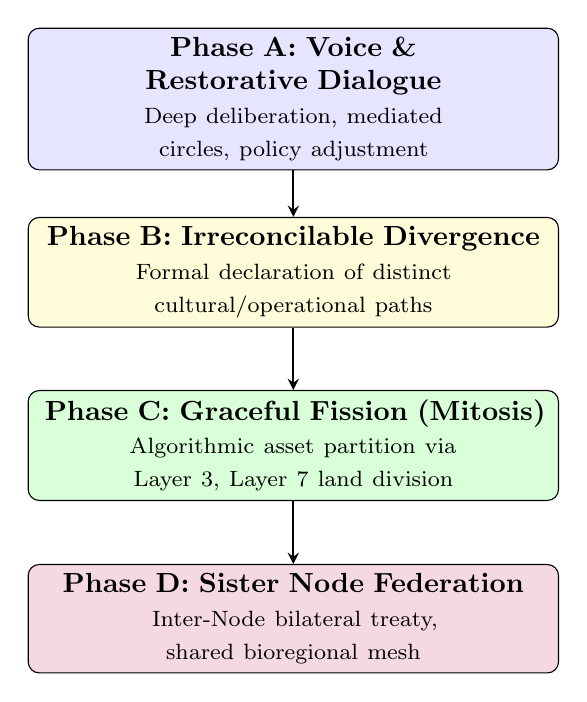
\begin{tikzpicture}[auto, >=stealth]
    \node [rectangle, draw, rounded corners, fill=blue!10, text width=6.5cm, text centered, minimum height=1cm] (voice) at (0, 0) {\textbf{Phase A: Voice \& Restorative Dialogue} \\ \footnotesize Deep deliberation, mediated circles, policy adjustment};
    \node [rectangle, draw, rounded corners, fill=yellow!15, text width=6.5cm, text centered, minimum height=1cm] (divergence) at (0, -2.2) {\textbf{Phase B: Irreconcilable Divergence} \\ \footnotesize Formal declaration of distinct cultural/operational paths};
    \node [rectangle, draw, rounded corners, fill=green!15, text width=6.5cm, text centered, minimum height=1cm] (fission) at (0, -4.4) {\textbf{Phase C: Graceful Fission (Mitosis)} \\ \footnotesize Algorithmic asset partition via Layer 3, Layer 7 land division};
    \node [rectangle, draw, rounded corners, fill=purple!15, text width=6.5cm, text centered, minimum height=1cm] (mesh) at (0, -6.6) {\textbf{Phase D: Sister Node Federation} \\ \footnotesize Inter-Node bilateral treaty, shared bioregional mesh};
    
    \draw [->, thick] (voice) -- (divergence);
    \draw [->, thick] (divergence) -- (fission);
    \draw [->, thick] (fission) -- (mesh);
\end{tikzpicture}
\caption{The lifecycle of graceful node fission (biological mitosis).}
\label{fig:node-fission}
\end{figure}

When a substantial faction within a Node determines that its core cultural, spiritual, or agricultural vision can no longer align with the Genesis Compact, it does not launch an internal coup. It initiates the \textit{Graceful Fission Protocol}:
\begin{enumerate}
    \item \textbf{Notice of Mitosis:} The diverging group files a formal petition in Layer~5, triggering a mandatory three-month reflection and mediation window.
    \item \textbf{Thermodynamic Asset Partitioning:} If reconciliation is not desired, the Layer~3 ledgers and Layer~4 Orchestrators calculate an equitable, mathematically verified partition of pooled capital, movable tools, solar infrastructure, and seed banks, proportionate to historical stewardship contributions and human need.
    \item \textbf{Spawning the Sister Node:} The departing group triggers Vector~3 of the Genesis Protocol (Chapter~9: Direct Layer~6 Mesh Expansion), acquiring adjacent or regional land under a new Community Land Trust to birth an autonomous Sister Node.
    \item \textbf{Bilateral Mesh Treaty:} The parent and sister nodes conclude an inter-node bilateral treaty, maintaining digital mesh interconnection, reciprocal emergency mutual aid, and open visiting rights, transforming an inevitable human conflict into a thriving, polycentric bioregional federation.
\end{enumerate}

\subsection{Neighborhood Assemblies vs. Technocratic Meritocracy}

A critical danger during bringup is the emergence of a technocratic gamer elite. If high-ranking Oasis players behave as self-appointed digital governors, the community will fracture into resentment.

The Sovereign Stack enforces strict anti-technocratic safeguards:
\begin{itemize}
    \item \textbf{The Primacy of the Neighborhood Assembly:} Sovereign political authority is anchored in the in-person, open Neighborhood Assembly \parencite{bookchin1982}. Non-gamers, elders, tenants, and youth possess equal voice and equal voting power with the most seasoned simulation players.
    \item \textbf{Gamers as Servant Facilitators:} Oasis players do not make decisions on behalf of the community. Their role is strictly logistical and consultative: they use their digital twin models to run predictive impact assessments for the assembly (e.g., showing projected thermodynamic trade-offs of different water harvesting layouts or solar arrays). They present options; the assembly decides.
    \item \textbf{Unmediated Spaces:} Under the Protocol of Refusal, the assembly may designate communal halls, dining spaces, gardens, and sacred grounds as permanently unmediated spaces, where all sensors, microphones, cameras, and data collection are strictly banned.
\end{itemize}


\section{From Game to Gateway: The Living Onboarding Pipeline}

In the final phase of collective bring-up, Oasis drops the commercial facade entirely. It ceases to be marketed as a commercial entertainment product and is recognized for what it truly is: the universal Semantic Interface (Layer~6) and educational onboarding gateway of The Collective \parencite{girard2013}.

The simulation remains perpetually active as a living digital twin. Before a physical community undertakes a hazardous real-world project---such as digging a keyline swale across a fragile watershed or rewiring a 480V three-phase solar microgrid---the community tests and rehearses the procedure inside the Oasis engine against simulated storm events and equipment failures. 

For newcomers seeking to transition out of the capitalist rat race, Oasis serves as the welcoming sandbox. Legacy citizens acquire foundational skills, build verified trust with living neighbors, and earn their first Verifiable Credentials in a risk-free digital environment. When they finally walk through the gates of a physical Sovereign Node, they are not strangers or unskilled laborers; they are already sovereign Stewards returning home to a world they have already helped build.


\chapter{A Minimum Viable Society: The 24 Scenarios}

In legacy software engineering, a product is launched by defining a Minimum Viable Product (MVP)---the smallest set of features necessary to deliver value. In the physical, thermodynamic architecture of The Sovereign Stack, we do not build products; we build civilizations. Therefore, we must define a \textit{Minimum Viable Society (MVS)}.

The MVS represents the baseline set of thermodynamic and sociological workflows that a Node must successfully execute to achieve localized autonomy. If a Node cannot master these foundational scenarios, it cannot survive without continuous, heavy reliance on the legacy capitalist supply chain (Layer 7). 

To systematically conquer these requirements, The Collective has defined 24 distinct scenarios, mapped from Alpha to Omega. These scenarios are currently undergoing rigorous Scenario-Driven Development (ScDD) within the Oasis simulation engine.


\section{Detailed Scenario Architectures}

To provide a concrete vision of what the Game Design Document (GDD) and the Scenario-Driven Development (ScDD) process entail, we provide a high-level architectural overview of the 24 foundational scenarios below. 

It is crucial to note that the following summaries serve merely as a narrative and structural baseline for the reader. The actual, deeply technical specifications for these scenarios are living artifacts of the game development process. Because they dictate the rigorous physics and governance of the Oasis engine, they are continuously managed, debated, refined, and distributed as living code repositories (currently hosted on GitHub, though the future inevitably reserves a decentralized medium for this governance). The 24 scenarios are not static gospel, but an evolving, iterative blueprint for systemic survival.

\subsection{Scenario Alpha ($\alpha$): The Fabrication Commons}

Imagine a sprawling suburban street where fifty closed garages hide fifty identical power drills, silently gathering dust in plastic cases. Each drill will be used for barely twelve minutes over its entire lifespan. This is the silent tragedy of atomized consumerism---a massive, systemic waste of planetary exergy, lithium, and rare earth metals, driven by a legacy culture that prioritizes isolated ownership over collective capability.

Scenario Alpha shatters this isolation by establishing the Fabrication Commons: a brightly lit, hum-filled neighborhood hub smelling of warm PLA plastic, sawdust, and machine oil. When a Steward needs to repair a broken appliance or mill a custom bracket, they do not drive to a big-box store to buy another cheap, disposable tool. Instead, they pull up their local Agora and emit a \textit{FabricationIntent} (Layer 6), requesting access to the community's high-end CNC machines, multi-axis 3D printers, and robust, shared lending library.

There is no tired human manager holding the keys. Access is smoothly and invisibly governed by Layer 5 Verifiable Credentials. The Sovereign Stack ensures that a novice Steward cannot simply walk in and activate a high-temperature induction furnace or a dangerous reciprocating saw; the system strictly demands cryptographic proof of their safety training. Behind the scenes, the Orchestrator (Layer 4) hums quietly, seamlessly scheduling bookings and queuing print jobs so that the Commons operates like a perfectly choreographed ballet, free of localized bottlenecks.

The magic truly manifests in the physical execution. As a Steward walks up to an IoT-enabled smart locker, it flashes green and physically unlatches, responding to their cryptographically signed Bluetooth telemetry (Layer 2). Inside the fabrication bays, edge-AI cameras watch extruded parts take shape, instantly halting jobs to prevent wasted plastic if a structural failure is detected. As the spindle spins and the filament melts, the Orchestrator calculates the precise grams of material used and the microscopic wear on the machine belts, routing the exact exergy bill directly to the Thermodynamic Ledger (Layer 3). The Steward walks away with a finished physical part, having engaged in a localized, zero-debt act of pure physical creation.

\subsection{Scenario Beta ($\beta$): Decentralized Transit}

Picture a six-lane legacy highway at 8:00 AM, choked with idling metal. Inside each 4,000-pound steel cage sits a single human, burning irreplaceable petrochemicals to move mostly empty air. Meanwhile, corporate gig-economy platforms extract massive platform fees just to match riders with a few of those empty seats. This is a thermodynamic atrocity disguised as modern convenience, fueled by isolated ownership.

Scenario Beta reclaims physical mobility by matching temporal-spatial vectors directly through the local mesh. When a Steward emits a \textit{TransitIntent} (Layer 6) from their device, there is no corporate algorithm matching them with a stranger for profit. The system simply asks the physical truth: who in the community is going this exact way, and how can we share the thermodynamic load?

The Orchestrator (Layer 4) acts as a ruthless physics engine. It calculates the exact exergy cost of a detour; if picking up a passenger wastes more vehicle energy than it saves in aggregate, the match is rejected. Safety, the historical moat of legacy platforms, is handled elegantly by Layer 5. You do not ride with random strangers; you ride only with mathematically verified peers connected through your Trust Ring, while the Layer 7 SPC acts as a commercial insurance shield for the entire community fleet.

The physical execution is entirely frictionless. For peer-to-peer vehicle lending, Layer 2 provisions a temporary, cryptographically signed Bluetooth key. A Steward walks up to a neighbor's parked EV, their phone flashes, and the door quietly unlocks. Layer 3 escrows the exact kilowatt-hours of battery depleted and the fractional tire wear, settling the transaction the exact moment the car is parked again, proving that localized logistics require zero corporate extraction.

\subsection{Scenario Gamma ($\gamma$): The Commons Kitchen}

The legacy food system is a marvel of ecological devastation. A single bell pepper travels 1,500 miles via refrigerated diesel trucks, wrapped in single-use plastic, only to be delivered to an atomized apartment by an exhausted gig-worker for a 30\% markup. Meanwhile, municipal bureaucrats enforce rigid zoning laws that outlaw neighborhood ``cottage'' kitchens in favor of highly capitalized, stainless-steel commercial franchises.

Scenario Gamma shatters this fragile supply chain by restoring the ancient hearth. The Commons Kitchen is a localized, bustling hub filled with the scent of roasted local vegetables and simmering broth. Instead of isolating consumers, it orchestrates hyper-local meal preps, matching the surplus yields of neighborhood permaculture plots directly with community chefs who transform them into highly nutritious, exergy-efficient meals.

The Orchestrator (Layer 4) manages the logistics with zero waste, ensuring that freshly harvested heirloom tomatoes do not rot in a pantry but are immediately routed into the day's menu. But the true breakthrough is how the Node bypasses legacy health inspectors: it relies on continuous, mathematically inviolable thermal telemetry. Layer 2 smart probes are embedded directly into the ovens, vats, and cold-storage units.

These probes stream the exact cooking temperatures in real-time to the Ledger, providing cryptographic proof that the food reached a safe 165$^{\circ}$F. This immutable telemetry satisfies Layer 7 regulatory requirements without requiring centralized permission. When the hot meals are finally served at the communal tables, Layer 3 routes Exergy Credits directly to the growers and chefs. The caloric and economic energy remains entirely within the neighborhood, deeply nourishing the physical and social fabric of the Node.

\subsection{Scenario Delta ($\delta$): Mutual Aid Childcare Pod}

The nuclear family model has deeply isolated modern parents, turning childcare into a crushing financial and emotional burden. Picture exhausted parents living in isolated suburban boxes, handing over half their salary to a commercial daycare where underpaid workers manage impossible ratios. It is a system that extracts fiat from desperate families while structurally devaluing the very act of raising the next generation.

Scenario Delta shatters this isolation by establishing the mutual aid childcare pod: a sunlit living room or community garden where care is shared collectively. When parents emit a \textit{ChildcareIntent}, the Orchestrator does not route them to a centralized corporation. Instead, it balances the temporal availability of a localized pod, mathematically ensuring labor equity so parents can trade shifts caring for a small, intimately connected group of children.

Because nothing requires a higher level of systemic trust than a child, Layer 5 Kinship routing is exceedingly strict. A childcare pod is not open to the general mesh; it is a highly guarded, multi-signature Trust Ring. Parents and vetted caretakers must cross-verify each other's credentials in the physical world and establish absolute cryptographic consensus before a pod is formed, guaranteeing safety without state bureaucracy.

Crucially, Layer 3 recognizes this caregiving---labor historically unpaid and marginalized by capitalism---as foundational thermodynamic work. When a parent handles a morning shift of education and care, the system mathematically logs this contribution. They are compensated directly in Exergy Credits, allowing them to purchase food from the Commons Kitchen (Gamma) or tools from the Fabrication Commons (Alpha). Raising a human is finally recognized by the ledger as the ultimate act of systemic negentropy.

\subsection{Scenario Epsilon ($\varepsilon$): Sovereign Third Place (Coworking)}

Late-stage capitalism has systematically eradicated the ``Third Place.'' Commercial real estate rent ensures that only profitable legacy businesses can maintain physical square footage, leaving neighborhoods with empty corporate offices, dead strip malls, and coffee shops that require a \$7 latte just for the right to sit down. Communities have literally nowhere left to gather for free.

Scenario Epsilon utilizes spatial multiplexing to reclaim the physical world. Picture a retrofitted garage, a vacant lot, or a community hall that acts as a quiet, sunlit coworking space at 10:00 AM, transforms into a Fabrication Commons at 2:00 PM, and becomes a bustling, music-filled poetry slam at 8:00 PM. By emitting a semantic intent (Layer 6), the community seamlessly flips the physical purpose of the space.

Access control is managed automatically and securely. There is no human bouncer or landlord holding a master key. Instead, Layer 2 BLE beacons verify a user's Layer 5 credentials at the door, quietly unlocking the physical actuators. The Orchestrator (Layer 4) manages the schedule, preventing double-bookings and ensuring that heavy machinery workflows do not overlap with quiet study hours.

To sustain the space, the Ledger (Layer 3) simply bills the specific event or guild for the exact thermodynamic energy (electricity, heating, water) consumed during their time slot, tracked flawlessly by Layer 2 HVAC sensors. The physical maintenance of the Third Place is perfectly subsidized by its active users, entirely bypassing the concept of commercial rent.

\subsection{Scenario Zeta ($\zeta$): Micro-Lodging Mesh}

Corporate platforms like Airbnb initially promised a peer-to-peer sharing economy, but rapidly degenerated into predatory rent extraction. They hollowed out local housing markets, turned residential neighborhoods into sterile hotel districts, and extracted massive platform fees while leaving the actual hosts and travelers to shoulder the physical risk. 

Scenario Zeta routes temporary lodging through the localized mesh, prioritizing mutual aid over rent extraction. Picture an itinerant Steward arriving in a new city and walking directly into a cozy, locally built micro-cabin or a spare room in a community house. They emitted a \textit{LodgingIntent} on Layer 6, and were welcomed not as a paying customer, but as a peer in a global network.

Instead of a centralized algorithm reading fake reviews, Layer 5 Trust Rings verify the traveler's reputation across the global mesh. A host can cryptographically verify that the traveler did not trash their last stop before accepting the request. The Orchestrator handles the booking, ensuring the host is prepared for the arrival.

The physical handoff is seamless. Layer 2 provisions a temporary Bluetooth key to the traveler's device, unlocking the smart lock at the door. Layer 3 tracks the excess water and energy consumed during the stay, and settles the transaction in Value Tokens directly between the peers. Zero platform fees are extracted, starving the legacy monopolies while fostering genuine, trust-verifiable hospitality.

\subsection{Scenario Eta ($\eta$): Coppice \& Carbon Commons}

The legacy material economy relies on industrial clearcutting, liquidating ancient forests simply to produce disposable paper cups and cheap, rotting suburban frames. It treats the living biosphere as an infinite mine, accelerating ecological collapse while trapping communities in a fragile dependency on global lumber supply chains.

Scenario Eta reclaims raw material production by establishing the Coppice and Carbon Commons. Picture Stewards walking into a quiet, meticulously managed bamboo grove or a thriving coppice forest. Here, they engage in the regenerative harvesting of local timber and bio-fibers. They are not clearcutting; they are pruning and selectively harvesting materials that will rapidly regrow, providing local feedstock for fabrication and construction.

The Orchestrator (Layer 4) serves as the relentless guardian of the forest. It refuses to generate a harvest workflow if the ecological battery is low. It relies on the Digital Twin (Layer 2) to ingest continuous telemetry on soil moisture, carbon sequestration, and sapling regrowth rates, ensuring that extraction never outpaces the forest's thermodynamic replacement rate.

The Stewards who perform the grueling, physical labor of forestry and processing are heavily rewarded by the Ledger (Layer 3). They earn significant Exergy Credits for their sweat, ensuring the community maintains a steady, ecologically sustainable supply of physical feedstock while completely decoupling from the legacy lumber industry.

\subsection{Scenario Theta ($\theta$): Neighborhood Micro-Foundry}

Every year, mountains of toxic e-waste and scrap metal are shipped to the global south to be burned in open pits or buried in landfills. The legacy system produces technological wonders, but possesses absolutely no mechanism for circular recovery, treating highly refined metals as disposable trash.

Scenario Theta is the metallurgical heart of The Collective. Picture a localized, heavily ventilated workshop glowing with the intense heat of an induction furnace and the sparks of a CNC plasma cutter. Here, Stewards melt down legacy e-waste, aluminum chassis, and scrap steel, literally liquidating the detritus of the legacy world to cast the structural backbone of the new one.

Because this involves highly dangerous temperatures and toxic off-gassing, Layer 5 demands extreme cryptographic safety credentials before granting a Steward access to the foundry workflow. The Orchestrator strictly monitors who is allowed to operate the crucibles, ensuring localized heavy industry remains incredibly safe.

The Digital Twin (Layer 2) is hyper-vigilant. Localized air quality sensors and thermal cameras constantly monitor the physical space; if safety thresholds are breached, Layer 2 instantly shuts down the electrical actuators powering the furnaces. The extracted raw materials (copper ingots, aluminum blocks) are then tokenized into Layer 3 as raw material credits, closing the loop on physical manufacturing.

\subsection{Scenario Iota ($\iota$): The Epistemic Mesh (R\&D)}

Intellectual property in the legacy world is heavily hoarded by corporations and trapped behind expensive academic paywalls. Brilliant engineers are gagged by Non-Disclosure Agreements, and life-saving research is hidden away to maximize quarterly profits, artificially stifling global innovation and trapping humanity in a slow, proprietary dark age.

Scenario Iota shatters this hoarding by establishing the protocol for decentralized, open-source scientific research. Imagine a local Node solving a unique physical problem---such as optimizing a 3D-printed solar water pump for a specific arid climate. Instead of patenting it, they immediately publish the exact BPMN workflow, Layer 2 sensor configurations, and 3D CAD files to the global Layer 6 Semantic Agora.

The network functions as a massively parallel, decentralized engineering firm. Other Nodes across the planetary mesh can freely download, test, and improve these designs, bypassing corporate R\&D entirely. The Orchestrator (Layer 4) tracks the forks and merges of these physical blueprints, ensuring quality control across the global mesh.

The Ledger (Layer 3) handles the incentive structure flawlessly. It tracks the cryptographic provenance of these ideas. Whenever the research is successfully deployed by a sister Node---perhaps halfway across the world in a similar desert---the original creators are retroactively rewarded with Reputational Wealth (Layer 5) and Exergy. This fundamentally aligns brilliant minds to open-source their life's work for the survival of the species.

\subsection{Scenario Kappa ($\kappa$): The Apprenticeship Protocol}

The legacy education system is a debt-trap. Teenagers are coerced into taking on \$100,000 in fiat student loans to sit in theoretical classrooms that are fundamentally disconnected from physical reality, only to graduate into a precarious gig economy. Education has been financialized into a highly extractive, abstract industry.

Scenario Kappa re-establishes the ancient master-apprentice dynamic, managed entirely debt-free via the Sovereign Stack. Picture a dusty workbench where a Master Steward patiently shows a teenager how to properly solder a motherboard, or how to listen to the pitch of an induction furnace to know when the metal is ready to pour. It is a return to tacit, physical knowledge transfer.

A master (holding high-level Layer 5 credentials in a specific discipline) agrees to take on the apprentice. The Orchestrator (Layer 4) tracks the syllabus, logs the hours worked, and manages the milestones of the final capstone project. Upon completion, Layer 5 mathematically issues the new Verifiable Credential to the apprentice.

The exchange is purely thermodynamic. The master expends high-value instructional exergy, while the apprentice provides low-level kinetic energy (cleaning the shop, prepping materials, organizing inventory). Layer 3 tracks this physical labor flawlessly, routing Exergy Credits to the master and settling the entire educational transaction locally without a single cent of fiat debt.

\subsection{Scenario Lambda ($\lambda$): Cultural Commons (Morale)}

A civilization cannot survive on raw thermodynamics alone; it requires psychological negentropy. Yet the legacy world isolates us into passive consumption, watching Netflix alone in our rooms, while draconian Homeowner Associations (HOAs) call the police on teenagers practicing drums in their own garages. Culture has been monopolized by corporate platforms like Spotify and Ticketmaster.

Scenario Lambda reclaims active culture and somatic play. Picture a vibrant neighborhood concert under string lights, a fiercely contested 3v3 basketball game on a local court, or an immersive tabletop storytelling campaign in the coworking space. By emitting a semantic intent (Layer 6), the community actively schedules and physically manifests its own entertainment.

The Orchestrator (Layer 4) manages the spatial and acoustic budgets of the Node. Using Layer 2 decibel telemetry at the property boundaries, it ensures that the live concert does not violate the acoustic limits of the sleeping neighbors in the next block. If the HOA complains, the Layer 7 SPC instantly provides cryptographic proof that local noise ordinances were never breached.

Furthermore, the Ledger (Layer 3) directly mints Value Tokens to the artists, musicians, and athletes from a communal Morale Fund. Culture is mathematically recognized not as a luxury, but as a critical systemic asset required to prevent burnout and ensure the psychological survival of the mesh.

\subsection{Scenario Mu ($\mu$): Regenerative Extraction (Biochar \& Biodigestion)}

The legacy waste system commits two profound thermodynamic crimes. First, organic biomass is landfilled to rot into methane, releasing stored carbon into the atmosphere. Second, vital human and animal biological waste---rich in nitrogen and phosphorus---is literally flushed away using purified drinking water. This forces local agriculture to rely on imported, destructive petrochemical fertilizers, stripping the soil microbiome until it is nothing but dead, dusty dirt.

Scenario Mu coordinates the high-heat physics and biological inoculation required to close this loop. Picture a localized retort kiln safely burning yard waste into biochar---locking carbon into a highly porous, stable lattice that lasts for millennia. Nearby, thermophilic composters safely process humanure and pet waste. The true magic occurs when these elements merge. Stewards introduce red wiggler worms and mycelial spores into the cooled compost and raw biochar. The worms digest the waste, coating the carbon lattice in a thriving microbiological biofilm to create ``Terra Preta,'' an incredibly nutrient-dense, water-retaining soil sponge.

Layer 5 handles the immense biological risk associated with this process. Handling human waste requires flawless pathogen control. Layer 5 mandates that any compost intended for food-bearing soil must hold cryptographic Layer 2 telemetry proving it sustained thermophilic temperatures (over 131$^{\circ}$F) for at least three consecutive days to kill all pathogens. If the heat curve fails, the Orchestrator mathematically locks the compost from agricultural use.

In the physical realm, the Orchestrator acts as both the kiln and the biological operator. It tracks the thermal cooling phase to ensure the compost is safe before Stewards introduce the delicate soil microbiome. Because this process physically locks carbon out of the atmosphere, the Layer 7 SPC packages the Node's Layer 2 telemetry into cryptographic proofs, selling them on legacy carbon markets for fiat. This elegantly uses the legacy financial system to directly fund the community's sovereign microbiological regeneration.

\subsection{Scenario Nu ($\nu$): Circular Modular Fashion}

Fast fashion is one of the most toxic industries on the planet. Garments are woven from micro-plastics in sweatshops, shipped across oceans, worn a handful of times, and then dumped into massive landfills in the global south. The legacy consumer is trained to treat clothing as disposable, extracting value from marginalized labor and destroying local textile resilience.

Scenario Nu reclaims the loom by establishing a localized, circular fashion and repair protocol. Picture a neighborhood textile hub humming with the sound of industrial walking-foot sewing machines. Here, Stewards engage in high-end visible mending, bespoke tailoring, and the fabrication of modular canvas gear (like e-bike saddlebags or micro-cabin tents) using open-source parametric patterns from the Agora.

Because industrial sewing equipment can easily cause physical injury or be destroyed if mistreated, Layer 5 tightly restricts physical power to the machinery unless the user holds a \textit{Textile\_Machinery} Verifiable Credential. The Orchestrator routes repair bounties to the appropriately skilled Stewards, ensuring zero-waste logic: natural scraps go to Scenario Mu for biochar, while synthetic scraps are routed to Scenario Theta to be melted into 3D printer filament.

The Ledger (Layer 3) mathematically incentivizes mending over replacement. By repairing a torn jacket, a Steward stops the entropic decay of a physical asset, and the Ledger compensates their localized labor with Exergy Credits. It restores dignity to the artisan, breaking the fast-fashion supply chain by making repair economically superior to consumption.


\subsection{Scenario Xi ($\xi$): Algorithmic Architecture}

Picture an endless, culturally sterile suburban sprawl of fragile houses glued together with toxic chemicals, bleeding heat into the winter air. The legacy construction industry relies on high-entropy global supply chains, mass-producing structures that entirely ignore local microclimates. Furthermore, attempting to retrofit these inefficient buildings is a bureaucratic nightmare, trapped behind expensive contractors and rigid municipal zoning boards that prioritize aesthetic conformity over ecological survival.

Scenario Xi hacks the modern world from within by treating the physical landscape as a parametric canvas. It uses open-source algorithms to dynamically augment, subdivide, and retrofit the existing urban landscape. When a Steward emits a \textit{RetrofitIntent}, they do not order standardized lumber from a big-box store. Instead, they scan their physical environment, and the Agora computes a structurally sound, custom geometry perfectly optimized for the exact localized materials the Node has on hand---down to the specific irregular logs harvested in Scenario Eta.

The Orchestrator (Layer 4) serves as the master builder, immediately breaking the generated CAD model into a precise Bill of Materials. It routes requests across the mesh: to the Fabrication Commons (Alpha) for 3D-printed structural nodes, and to the Micro-Foundry (Theta) for cast brackets. Crucially, Layer 5 enforces a strict ``Deconstruction Mandate''---prohibiting chemical glues in favor of modular bolts and pegs, mathematically guaranteeing the building can be effortlessly dismantled and reused at the end of its lifecycle to prevent landfill waste.

Before a single physical board is cut, the Digital Twin (Layer 2) runs thousands of passive solar and wind-load simulations. If the physics engine detects a thermodynamic violation---such as a window placement causing massive winter heat loss---it rejects the design outright. When construction finally begins, the Layer 7 SPC absorbs the municipal permit fees and legally shields the decentralized labor force. The community gathers for a modern, localized barn-raising, settling the transaction not with a 30-year fiat mortgage, but by instantly rewarding the physical builders with Layer 3 Exergy Credits.

\subsection{Scenario Omicron ($o$): The Kinship Protocol (Trust Rings)}

In the legacy system, trust is outsourced to centralized data brokers (Experian) or state authorities (KYC). More insidiously, this legacy system deliberately merges human survival with economic coercion; if someone leaves an abusive partner or a toxic workplace, they risk homelessness and starvation. Early ``Web3'' systems risk recreating this dystopia via un-erasable, panoptic social credit scores where the wealthy can weaponize their reputation to coerce the vulnerable.

Scenario Omicron fundamentally solves this by establishing ``Trust Rings.'' You cannot simply spin up a fake digital identity to book 3D printers or participate in childcare; your Decentralized Identifier must be cryptographically attached to the human social graph via physical ``vouching.'' Picture two Stewards exchanging cryptographic NFC handshakes on their phones after sharing a meal in the Commons Kitchen (Scenario Gamma)---breaking bread mathematically authenticates the physical bond.

Layer 5 creates a profound ``Basic Needs Firewall.'' Trust Rings strictly govern access to high-risk, high-exergy assets (like borrowing an EV or operating industrial foundries). If a Steward vouches for a bad actor who vandalizes the foundry, both users face ``Social Slashing.'' However, Layer 5 strictly prohibits gating \textit{survival resources} (food, emergency shelter, medical care) behind reputation. You cannot starve someone by downvoting them.

Crucially, to protect intimacy from coercion, the protocol features a cryptographic Safe Harbor. If a relationship turns toxic, a Steward can execute a \textit{SeveranceIntent}. This elegantly severs the graph edge without triggering a slashing penalty, mathematically preventing high-reputation users from holding someone's social status or housing access hostage. It ensures the Web of Trust protects the commons without ever coercing the individual.


\subsection{Scenario Pi ($\pi$): The Sovereign Guild (Identity \& Treasury)}

In the legacy economy, independent labor is deeply precarious. Freelancers navigate a maze of disparate 1099 contracts, expensive private health insurance traps, and predatory gig-economy platforms. You are treated as a disposable, atomized contractor, stripped of the collective bargaining power that historically protected the working class.

Scenario Pi rebuilds the union through the Sovereign Guild. Picture a highly skilled collective of engineers, writers, and fabricators operating as a localized guild. When they emit a \textit{GuildIntent}, they do not bid against each other in a race to the bottom. Instead, they pool their skills to take on massive legacy contracts---building software for Web2 companies or fabricating hardware---as a unified, cybernetic entity.

The orchestration of this labor is seamless. The Layer 7 SPC acts as the legacy Employer of Record, absorbing the fiat payments, handling tax compliance, and providing blanket healthcare for the Guild members. Inside the mesh, Layer 5 Polycentric governance allows the Guild to vote cryptographically on how to allocate the pooled surplus, completely sidestepping corporate HR departments.

In the physical realm, the Orchestrator (Layer 4) breaks the massive legacy contract into localized tasks, routing them to the relevant Stewards. As the work is completed, Layer 3 acts as the grand converter---translating the ingested legacy fiat directly into internal Exergy Credits, effectively siphoning economic energy out of late-stage capitalism to physically fund the Node's autonomous infrastructure.

\subsection{Scenario Rho ($\rho$): The Adversarial Mesh (Threat Defense)}

The legacy system's approach to security is heavily centralized and often disastrously brittle. Digital security relies on centralized corporate servers that are regularly breached, while physical security relies on state police forces that arrive twenty minutes after a crime has occurred. Furthermore, alternative communities are uniquely vulnerable to targeted legal harassment, state inspections, or localized vandalism.

Scenario Rho tests the Node's ability to survive when the environment becomes actively hostile. Imagine a scenario where a bad actor attempts a digital Sybil attack, or a legacy state inspector arrives unannounced demanding access to the Fabrication Commons. The Node does not panic; it executes a mathematically rigorous defense protocol.

Upon detecting a threat, a Steward emits a \textit{LockdownIntent}. The Orchestrator (Layer 4) immediately triggers defensive workflows. Layer 5 Trust Rings dynamically contract---privileges for lower-tier members are temporarily suspended, and high-exergy systems are cryptographically locked, requiring an immediate multi-signature override from the core Stewards to operate.

The Digital Twin (Layer 2) executes the physical defense. Smart locks sever their Bluetooth connections, physically isolating sensitive hardware like the micro-foundry or servers. Simultaneously, the Layer 7 SPC legally shields the Node, presenting the state inspector with a perfectly compliant, sanitized legacy proxy, while the true thermodynamic and cryptographic operations of the Node remain completely opaque and untouchable behind the firewall.

\subsection{Scenario Sigma ($\sigma$): Altruism Fatigue (Burnout)}

The greatest tragedy of legacy mutual aid and activist spaces is not a lack of funding, but the structural collapse of human energy. Capitalism externalizes maintenance. In voluntary spaces, the same three people inevitably do all the sweeping, cooking, and organizing until they emotionally break. This "altruism fatigue" destroys more communities than external hostility ever could.

Scenario Sigma structurally prevents this collapse by treating human psychological energy as a finite, measurable resource. Picture the localized chore wheel---a \textit{MaintenanceBounty} to deep-clean the Commons Kitchen or empty the heavy ash bins of the biochar retort. Instead of relying on guilt to get the job done, the Orchestrator (Layer 4) acts as an algorithmic manager that cannot be ignored.

If an unpleasant task remains unclaimed, the Orchestrator initiates a Dutch Auction. It systematically escalates the Value Token reward until the thermodynamic incentive mathematically matches a citizen's willingness to perform the low-status labor. Crucially, Layer 3 subsidizes this invisible maintenance labor heavily, allowing a Steward to feed themselves for a week simply by maintaining the hygiene of the physical commons.

To prevent self-immolation, Layer 5 employs a "Fatigue Lockout." If a Steward claims 80\% of the cleaning bounties in a month, the system detects approaching burnout. The Trust Ring mathematically locks them out of accepting new maintenance bounties and suggests a `RestIntent` or participation in the Cultural Commons (Lambda), forcing the rest of the network to step up and recognizing human rest as a critical systemic imperative.

\subsection{Scenario Tau ($\tau$): Steward Genesis (Character Creation)}

In the legacy system, onboarding into society is coercive and deeply extractive. Your identity is reduced to a credit score, a criminal background check, and a corporate resume. When you move to a new neighborhood, your actual utility---your tools, your tacit skills, your willingness to help---remains completely invisible to the people living fifty feet away.

Scenario Tau is the "Genesis Protocol," the character creation screen of the physical world. Picture a newcomer arriving at an established Node. They emit a \textit{GenesisIntent}, boldly declaring their physical reality to the local mesh: "I am bringing a table saw, a spare bedroom, and five years of permaculture experience." They are digitizing their physical assets into a secure, trust-based pathway.

Because the system cannot afford a "cold start" vulnerability, this onboarding is deeply physical. Layer 5 requires a Key-Signing Party with an existing Sponsor---a Steward who stakes their own Reputational Weight to grant the newcomer their initial cryptographic credentials, linking their Decentralized Identifier to the human social graph.

Once vetted, the physical world integrates seamlessly. The newcomer uses their device to scan their tools, instantly generating Layer 2 digital twins of their assets. To ensure they can survive day one, Layer 3 initializes a "Seed Escrow"---a micro-loan of Value Tokens that allows the newcomer to purchase a meal at the Commons Kitchen (Gamma) or book a tool (Alpha) immediately, seamlessly weaving a legacy human into a fully operational cybernetic society.


\subsection{Scenario Upsilon ($\upsilon$): The Exergy Shock (Blackout \& Resilience)}

The legacy utility grid is an incredibly brittle, centralized monolith. When a freak winter storm or a heatwave triggers a grid collapse, legacy homes instantly freeze or overheat. Atomized neighbors, entirely dependent on a profit-driven utility company, panic-buy resources while waiting helplessly for the state to restore power.

Scenario Upsilon tests the Node's ability to survive catastrophic external failure. When the external power grid fails, the Orchestrator instantly detects the voltage drop via Layer 2 telemetry and emits a \textit{GridFailureIntent}. The Node executes "Islanding Mode," physically severing its connection to the legacy grid and seamlessly transitioning to its localized solar, wind, and battery arrays.

Governance (Layer 5) immediately executes "Life Support Triage." All high-exergy, low-priority activities are mathematically shut down. A Steward attempting to run a CNC machine in the Fabrication Commons (Alpha) will find the physical actuators locked out. Power is ruthlessly routed to critical survival infrastructure: keeping the medical fridges cold in the Paramedic Mesh (Chi) and maintaining the thermal baseline in the Micro-Lodging (Zeta).

The Ledger (Layer 3) tracks the precise draw on the localized thermodynamic battery, ensuring the community survives the deep freeze. The Node operates as a sovereign, impenetrable micro-grid, turning a disaster that would destroy a legacy suburb into a minor, mathematically managed inconvenience.

\subsection{Scenario Phi ($\phi$): The Elder Protocol (Aging \& End-of-Life)}

The legacy paradigm for aging is horrifying. Elders are often stripped of their autonomy, warehoused in highly expensive, sterile corporate nursing homes, and drained of their fiat savings until they die in isolation. Aging is treated as a medicalized failure of productivity, rather than a crucial repository of systemic wisdom.

Scenario Phi reintegrates elders back into the beating heart of the Node. Picture a radically integrated, multigenerational environment where the emission of an \textit{ElderCareIntent} does not route an elder to a hospital, but surrounds them with localized, multi-generational mutual aid.

Because elders possess massive amounts of lived experience, Layer 5 grants them distinct "Wisdom Credentials." While they no longer perform heavy kinetic labor (like harvesting timber in Scenario Eta), they perform high-value cybernetic labor. They serve as neutral mediators (Scenario Psi), teach apprentices (Scenario Kappa), and act as the core stabilizing anchors of the Trust Ring. 

The Ledger (Layer 3) routes thermodynamic life support directly to them, honoring their decades of accumulated Reputational Wealth. Simultaneously, Layer 2 wearable telemetry detects falls or cardiac events instantly, dispatching localized care without relying on legacy emergency systems. The elder remains physically and socially embedded in the mesh until the end.

\subsection{Scenario Chi ($\chi$): The Paramedic Mesh \& Open-Source Pharmacopeia}

Medical care in the legacy world relies on dialing 911, waiting thirty minutes for a highly expensive, privatized ambulance, and then facing a \$50,000 emergency room bill. Beyond acute trauma, legacy medicine relies on centralized pharmaceutical monopolies that hoard life-saving compounds behind patents and extract massive fiat profit from prolonged sickness, deliberately financializing human suffering rather than prioritizing preventative health.

Scenario Chi deploys the localized Paramedic Mesh alongside an Open-Source Pharmacopeia. Picture a Steward suffering a deep laceration; their wearable instantly emits a \textit{TraumaIntent}. But Chi also handles preventative bio-hacking. Stewards can emit a \textit{SynthesisRequest} for a batch of open-source anti-inflammatory compounds or a 3D-printed insulin pump. To protect these local bio-hackers from federal FDA prosecution, the Layer 7 SPC legally classifies all synthesized compounds and hardware as ``Experimental Prototypes for Personal Use,'' completely bypassing legacy interstate commerce jurisdiction.

Layer 5 enforces absolute data privacy and strict competency gating. In legacy systems, health data is commodified; here, it is cryptographically sovereign. Layer 5 utilizes Zero-Knowledge (ZK) proofs, allowing a responding Paramedic to mathematically verify a patient is not allergic to a compound without ever gaining decryption access to their lifelong health ledger. Furthermore, Layer 5 restricts physical access to the Node's centrifuges and bio-reactors, ensuring only Stewards with rigorous \textit{Pharmacopeia} credentials can synthesize medicine.

When trauma occurs, the Orchestrator (Layer 4) immediately bypasses legacy routing, geolocating the nearest qualified responder and unlocking localized medical caches (oxygen, tourniquets). The trauma is stabilized in two minutes rather than thirty. The Ledger (Layer 3) then mints massive Exergy Credits to these heroic first responders. Crucially, the Ledger also pays Pharmacopeia practitioners based on \textit{preventative outcomes}---subsidizing health to keep the community entirely out of the extractive legacy hospital system.

\subsection{Scenario Psi ($\psi$): Restorative Mediation (Conflict Resolution)}

The legacy justice system is punitive, adversarial, and violently extractive. It relies on a state monopoly on violence (police) and ruinously expensive gatekeepers (lawyers). When a dispute occurs---whether a broken contract or a property line dispute---legacy courts focus on extracting fiat fines, fundamentally destroying the human relationship in the process. 

Scenario Psi establishes a decentralized arbitration and restorative justice protocol. When an interpersonal fracture occurs, a Steward emits a \textit{MediationIntent}. The Node recognizes that unresolved conflict acts as systemic friction (heat). If the community does not repair the social graph, the entire localized supply chain will eventually fail.

Layer 5 analyzes the Trust Ring graph to select a mediator. It mathematically searches for a Steward who has the exact same cryptographic distance (degrees of separation and vouch weight) from \textit{both} conflicting parties, ensuring absolute, undeniable neutrality. (If the intent flags intimate abuse, mediation is bypassed entirely in favor of the Safe Harbor protocol in Scenario Omicron).

Restitution is paid not in fiat fines, but in thermodynamic labor. The Orchestrator (Layer 4) assigns the offending party to Scenario Sigma (Maintenance). They must execute low-status cleaning bounties---scrubbing the kitchen, organizing the foundry---until their kinetic debt to the community is paid. The justice system repairs the social fabric through physical restitution rather than punitive extraction.

\subsection{Scenario Omega ($\omega$): Terminal Decoupling (The Sovereign Singularity)}

Layer 7 (the fiat corporate proxy) is a necessary evil during the Genesis phase, but relying on state-sanctioned property and fiat taxes forever is submission. The final evolutionary stage of a Node is to achieve complete physical and economic sovereignty, stripping fiat of its coercive power entirely.

Scenario Omega orchestrates the graceful deletion of the old world. Picture the moment the Node realizes its internal physical asset reserves (solar capacity, localized food production, micro-manufacturing) have crossed the "Sovereignty Threshold." The Node emits a \textit{TerminalDecouplingIntent}---the Singularity. 

The Trust Ring executes a massive, multi-sig transaction that legally dissolves the Layer 7 Social Purpose Corporation. The fiat bank accounts are permanently closed. The legacy legal entity ceases to exist, and the physical land transitions to pure cryptographic, polycentric stewardship. The fiat bridge is burned.

The Orchestrator (Layer 4) permanently drops all API webhooks to legacy banking and state databases. The Node now relies entirely on P2P LoRaWAN, dark fiber, and decentralized uplinks, routing pure thermodynamic exergy and data directly with other sovereign Nodes globally. The legacy state simply becomes irrelevant. The Collective is born.

\section{Iterative Engine Mastery \& Emergent Gameplay}

It is crucial to clarify that individual players within Oasis do not experience these 24 scenarios as a rigid sequence of linear ``levels'' or developer-scripted quests. Rather, it is the \textit{Game Development} process---via Scenario-Driven Development (ScDD)---that must rigorously conquer Alpha through Omega to prove the underlying physics engine is architecturally viable. 

To the player, Oasis is a boundless, open-world sandbox. It is a high-fidelity thermodynamic and sociological simulator disguised as a massively multiplayer online (MMO) game. Because the underlying engine has mastered the 24 foundational baselines of the Minimum Viable Society (MVS), the player's chosen environment can be wildly diverse. A player might govern an avatar in a high-density urban arcology, a sprawling suburban cooperative, a remote rural eco-village, a maritime flotilla, or a highly automated industrial foundry. 

In all of these environments, the 24 scenarios operate invisibly under the hood as the game's shadow architecture. A player might simply think they are opening a local bakery, fixing a neighbor's solar panel, or organizing a neighborhood concert, but beneath the surface, the engine is seamlessly firing off \textit{Gamma Intents}, routing \textit{Layer 5 Trust Ring} verifications, and settling thermodynamic debts on the \textit{Layer 3 Ledger}. There are no artificial Non-Player Character (NPC) quest givers; every localized supply chain, every conflict, and every alliance is driven by pure, emergent player behavior reacting to mathematically simulated scarcity.

Furthermore, the players themselves provide the ultimate, chaotic stress test for the Sovereign Stack. In any MMO, players will inevitably attempt to break the economy, hoard resources, grief their neighbors, or exploit algorithmic loopholes. This adversarial behavior is not a flaw; it is exactly what The Collective needs. By throwing tens of thousands of human minds into the simulation, we force the engine to dynamically resolve chaos via \textit{Scenario Psi (Mediation)} or \textit{Scenario Rho (Adversarial Defense)}. Every time a player discovers an exploit in the simulation, the developers patch the underlying cybernetic logic. 

Thus, the game serves as a massive evolutionary crucible. By the time the Oasis simulation is stable, balanced, and resilient against millions of hours of chaotic player behavior, we will have mathematically guaranteed that the Sovereign Stack is ready to be deployed into physical reality. As the ScDD process matures, subsequent volumes of this documentation will detail the specific mathematical, semantic, and cybernetic logic embedded within each of these 24 foundational scenarios.


\chapter{The Prime Genesis (Epilogue)}

We arrive, finally, at the paradox of the scaffolding. 

We cannot birth a fully sovereign, decentralized Node on Day 1 without relying on the very legacy corporate infrastructure we intend to obsolete. If we attempt to instantly apply the strict thermodynamic rules of the Sovereign Stack to our current reality---demanding that developers use mathematically pure JSON-LD intents rather than standard communication, or attempting to track early development via a physical exergy ledger---the project will collapse under bureaucratic friction and abstraction leaks. 

Instead, we must treat our current legacy environment as \textit{Temporary Scaffolding}. We will execute a phased decoupling, shedding legacy dependencies layer by layer as the Oasis Engine matures. This is the roadmap for ``Node 0''---the very first instantiation of The Collective.

\section{The Four Phases of Evolutionary Bootstrapping}

\subsection{Phase 1: The Brittle Approximation (Scaffolding)}
In this initial phase, we accept that we are entirely subservient to Layer 7 legacy infrastructure (e.g., GitHub, cloud servers, and fiat currency). The goal is raw velocity to build the foundational C++ Engine. 
\begin{itemize}
    \item \textbf{Layer 6 (Intent):} We use standard, unstructured text via legacy project management tools. We do not force humans to write machine-readable ontologies yet.
    \item \textbf{Layer 5 (Governance):} We use basic codebase repository permissions (like GitHub \texttt{CODEOWNERS}) as a brittle, centralized simulation of what will eventually become the Trust Ring.
    \item \textbf{Layer 4 (Orchestrator):} We rely on centralized corporate CI/CD pipelines to compile our WASM payload.
    \item \textbf{Layer 3 (Ledger):} We do not track tokens. We rely entirely on the unquantified, altruistic labor of the founding Stewards.
\end{itemize}

\subsection{Phase 2: The Hybrid Bridge (The Headless Engine)}
Once the C++ Engine is capable of running headless state machines, we begin routing actual logic \textit{through} it, though it remains hosted on legacy infrastructure.
\begin{itemize}
    \item \textbf{Layer 6 \& 4:} We introduce a bridge. A legacy ticket can now contain a JSON-LD block. A legacy script parses this block and feeds it directly into the headless Oasis Engine for validation. The BPMN engine begins to govern internal state, but legacy servers still act as the chronological trigger.
\end{itemize}

\subsection{Phase 3: The Sovereign Interface (Self-Hosting)}
The Oasis graphical client goes live and is capable of local P2P networking. The Node begins to govern itself using its own software.
\begin{itemize}
    \item \textbf{Layer 6 \& 4:} Legacy issue trackers are entirely deprecated for Node operations. Stewards use the Oasis UI to emit \textit{Intents} directly into the local CRDT mesh. The local C++ engine orchestrates the tasks without ever touching the cloud.
    \item \textbf{Layer 5 (Governance):} Centralized repository permissions are deprecated for operational trust. We transition to true cryptographic Key-Signing Parties (Scenario Omicron), linking digital identities to the physical human social graph.
\end{itemize}

\subsection{Phase 4: Terminal Decoupling (The Omega Scenario)}
This is the final shedding of the scaffolding, realizing the vision laid out in Scenario Omega.
\begin{itemize}
    \item \textbf{Codebase Migration:} The source code of the Oasis Engine is moved off centralized corporate servers entirely. It is natively distributed across the Node's own CRDT ledger or a decentralized P2P git protocol.
    \item \textbf{Layer 3 (Ledger):} The thermodynamic ledger is activated, tying actual physical exergy to the maintenance of the codebase and the physical infrastructure.
    \item \textbf{True Autonomy:} Node 0 exists purely on local hardware, governed by its own mathematical laws, completely illegible to and independent from the legacy state. The Singularity is achieved.
\end{itemize}

\section{The Call to Action}

This first volume serves as the theoretical and architectural bedrock of The Collective. But a blueprint, no matter how rigorous, cannot execute itself. 

The transition from late-stage capitalism to a thermodynamically sovereign society is the greatest engineering challenge of our generation. We are actively seeking the early adopters, the pioneers, and the system architects to help us build this reality. 

We need the C++ engineers to build the deterministic physics engine. We need the bio-hackers to map the Pharmacopeia. We need the permaculturalists to design the thermophilic composters. We need the game designers to build the Oasis interface that will seamlessly translate these complex cybernetic workflows into an intuitive, joyful human experience.

If you recognize the profound fragility of the legacy system---if you are exhausted by the extraction, the atomization, and the systemic decay of the modern world---we invite you to join us. We invite you to emit your own \textit{GenesisIntent}. 

Help us build the scaffolding, so that together, we can eventually burn it down.


\printbibliography

\end{document}
